%CLASSE DOCUMENTO - LINGUA E DIMENSIONE FONT
\documentclass[corpo=11pt,english,numerazioneromana]{toptesi}

%%%%%%%%%%%%%%%%%%%%%%%%%%%%%%%%%%%%%%%%%%%%%%%%%%%%%%%%%%%%%%%

% INCLUSIONE PACCHETTI
\usepackage[classica]{topfront}
\usepackage[utf8]{inputenc} %utf8
\usepackage[english]{babel}
\usepackage[T1]{fontenc}
\usepackage{blindtext}
\usepackage{graphicx,wrapfig}
\usepackage{booktabs}
\usepackage{lmodern}
\usepackage{varioref}
\usepackage{url}
\usepackage{multirow}
\usepackage{array}
\usepackage{paralist}{\obeyspaces\global\let =\space}
\usepackage{verbatim}
\usepackage{subfig}
\usepackage{tabularx}
\usepackage{amsmath}
\usepackage{amsfonts}
\usepackage{float}
\usepackage{amssymb}
\usepackage{multicol}
\usepackage{multirow}
\usepackage{listings}
\usepackage[pass]{geometry}
\usepackage[figuresright]{rotating}
\usepackage{algorithm}
\usepackage{algorithmic}
\usepackage{amsmath}
\usepackage[babel]{csquotes}
\usepackage{hyperref}
\usepackage[backend=biber,bibencoding=ascii, sorting=none, defernumbers]{biblatex}
\usepackage{enumitem}
\usepackage{colortbl}


%%%%%%%%%%%%%%%%%%%%%%%%%%%%%%%%%%%%%%%%%%%%%%%%%%%%%%%%%%%%%%%

% CONFIGURAZIONE LINK E RIFERIMENTI
\hypersetup{%
    pdfpagemode={UseOutlines},
    bookmarksopen,
    pdfstartview={FitH},
    colorlinks,
    linkcolor={black}, %COLORE DEI RIFERIMENTI AL TESTO
    citecolor={blue}, %COLORE DEI RIFERIMENTI ALLE CITAZIONI
    urlcolor={blue} %COLORI DEGLI URL
}

%%%%%%%%%%%%%%%%%%%%%%%%%%%%%%%%%%%%%%%%%%%%%%%%%%%%%%%%%%%%%%%

% CONFIGURAZIONE LISTATI/CODICE - CANCELLARE SE NON NECESSARIO
% PYTHON - BIANCO E NERO
\lstset{%
	captionpos=b,
	language=Python,
	basicstyle =\small\ttfamily,
	keywordstyle=\color{black}\bfseries,
	breaklines=true,
	breakatwhitespace=true,
	frame=lines,
	numbers=left,
	numberstyle=\footnotesize,
}

%%%%%%%%%%%%%%%%%%%%%%%%%%%%%%%%%%%%%%%%%%%%%%%%%%%%%%%%%%%%%%%

% FRENCHSPACING ABILITATO - CANCELLARE PER SPAZIATURA ALL'INGLESE
\frenchspacing

%%%%%%%%%%%%%%%%%%%%%%%%%%%%%%%%%%%%%%%%%%%%%%%%%%%%%%%%%%%%%%%

%DEFINIZIONE SEZIONI IN NUMERAZIONE ROMANA
%ELENCO DEI LISTATI/CODICI
\makeatletter
\newcommand\listofcodes{%
 \iffrontmatter\else\frontmattertrue\fi
 \if@openright\cleardoublepage\else\clearpage\fi
 % change the meaning of \chapter in a group
 \begingroup\def\chapter##1{\@schapter}
 \phantomsection % for the hyperlink
 \addcontentsline{toc}{chapter}{Listings}
 \lstlistoflistings 
 \endgroup
} 
\makeatother

%%%%%%%%%%%%%%%%%%%%%%%%%%%%%%%%%%%%%%%%%%%%%%%%%%%%%%%%%%%%%%%

% INFORMAZIONI PDF - PERSONALIZZARE
\pdfinfo{%
  /Title    (Foo Bar Baz)
  /Author   (Tinaso de Tinasis)
  /Subject  (How to write meaningful titles)
  /Keywords (LaTeXi foo bar baz meaningful PIT Presicce)
}

%%%%%%%%%%%%%%%%%%%%%%%%%%%%%%%%%%%%%%%%%%%%%%%%%%%%%%%%%%%%%%%

% LISTA DEI CAPITOLI DA INCLUDERE - PERSONALIZZARE
\includeonly{%
Introductions,%
Chapter1,%
Chapter2,%
Chapter3,%
Chapter4,%
conclusioni,%
appendix
}

% FILE DI BIBLIOGRAFIA
\addbibresource{bibliography.bib}

%%%%%%%%%%%%%%%%%%%%%%%%%%%%%%%%%%%%%%%%%%%%%%%%%%%%%%%%%%%%%%%

% INIZIO DOCUMENTO
\begin{document}
\english

%%%%%%%%%%%%%%%%%%%%%%%%%%%%%%%%%%%%%%%%%%%%%%%%%%%%%%%%%%%%%%%

% FRONTESPIZIO - PERSONALIZZARE
% ELIMINATE LE VOCI CHE NON VI SERVONO

% UNIVERSITA - NOME
\ateneo{Università degli Studi di Milano-Bicocca}

% FACOLTA - DICITURA
\FacoltaDi{Department of}
% FACOLTA - NOME
\facolta{Informatics, Systems and Communication}

% CORSO DI LAUREA - DICITURA (MANTENERE LO SPAZIO)
\CorsoDiLaureaIn{Master of Science in }
% CORSO DI LAUREA - NOME
\corsodilaurea{Data Science}

% TIPOLOGIA TESI
\TesiDiLaurea{Master Thesis}

% TITOLO
\titolo{Study of key Deep Learning techniques applied to Open Data for air quality monitoring in Smart Cities}



% RELATORE/I - DICITURA
\AdvisorName{Supervisor:}
% RELATORE - PROF. NOME E COGNOME
\relatore{Prof.\ Simone Bianco}
\secondorelatore{Prof.\ Paolo Napoletano}
\terzorelatore{Dr. Luigi Celona}
% RELATORE AGGIUNTIVO - PROF NOME E COGNOME
% SE SI HA SOLO UN RELATORE ELIMINARE E CAMBIARE Advisors in Advisor


% CANDIDATO - DICITURA (MANTENERE I DUE PUNTI)
\CandidateName{Candidate:}

% CANDIDATO - NOME E COGNOME
\candidato{Matteo Lanzillotti\\843283}

% LOGO UNIVERSITA
\logosede{images/logo}

% DATA - MESE ANNO
\sedutadilaurea{Academic Year 2022-2023}

\frontespizio

%%%%%%%%%%%%%%%%%%%%%%%%%%%%%%%%%%%%%%%%%%%%%%%%%%%%%%%%%%%%%%%

%INTERLINEA - DEFAULT 1 - NON ESAGERATE, NON SUPERATE MAI 1.3 ;)
\interlinea{1.5}

%%%%%%%%%%%%%%%%%%%%%%%%%%%%%%%%%%%%%%%%%%%%%%%%%%%%%%%%%%%%%%%

%\frontmatter

% DEDICA - PERSONALIZZARE
% VSPACE - PROPORZIONE USATA PER CENTRATURA VERTICALE DEL TESTO
% FLUSHRIGHT - ALLINEAMENTO ORIZZONTALE A DESTRA
%\vspace*{\stretch{1}}
%\begin{flushright}
%\noindent
%To me and only me
%\end{flushright}
%\vspace*{\stretch{6}}
%\cleardoublepage



%%%%%%%%%%%%%%%%%%%%%%%%%%%%%%%%%%%%%%%%%%%%%%%%%%%%%%%%%%%%%%%



% ABSTRACT - PERSONALIZZARE
%\sommario
%Abstract, pleased to meet you. Ah, it's not funny anymore.

%%%%%%%%%%%%%%%%%%%%%%%%%%%%%%%%%%%%%%%%%%%%%%%%%%%%%%%%%%%%%%%

% INDICI - ELIMINARE GLI INDICI NON NECESSARI

% INDICE GENERALE
\tableofcontents
\chapter*{Introductions}
\addcontentsline{toc}{chapter}{Introductions}

In contemporary smart cities, the integration of technology and data is reshaping the way we live. However, concerns regarding air quality are escalating, necessitating innovative and accurate forecasting techniques for air pollutant concentrations. The dynamics of urban environments, coupled with the complexity of pollutant sources, pose a formidable challenge for traditional forecasting methods. This master's thesis explores the use of deep learning techniques to predict air pollutant concentrations, with the goal of improving the accuracy and flexibility of forecasting models in the dynamic environment of smart cities. This research aims to develop robust and efficient tools for proactive air quality management by utilizing advanced neural networks. The goal is to provide decision-makers with timely and actionable insights to promote healthier and more sustainable urban living environments.

\section*{Background and Motivation}

The impact of air pollutants on public health is a critical concern in urban areas. Therefore, it is imperative to adopt a proactive and comprehensive approach to managing air quality. This is especially crucial in the context of smart cities, where technological advancements seamlessly integrate into urban infrastructure, underscoring the need to monitor and address air quality issues. Equipped with an array of sensors and data-driven technologies, smart cities offer an unprecedented opportunity to continually monitor air quality in real-time. However, the sheer volume, diversity, and intricacy of data generated in these smart environments present a substantial challenge for conventional forecasting methods. To bridge this gap, the study employs deep learning techniques known for their proficiency in handling vast and complex datasets. The objective is to improve the accuracy and flexibility of models that forecast air pollutant concentrations. The data collected in smart cities is rich and varied, and coupled with the multifaceted nature of pollutant sources, it emphasizes the necessity for advanced computational methods to extract valuable insights. Consequently, this research aims to combine health-conscious urban planning with advanced technology. Deep learning will be used to analyze air pollutants concentrations in the context of smart cities.

\section*{Methodologies}

The study employs a comprehensive methodology to analyze real-world data sets, with the aim of uncovering patterns and dynamics. Three distinct data sets are examined, each presenting unique challenges. The first phase introduces these data sets, outlining their unique attributes and contextualizing subsequent analyses within their complexities. This lays the groundwork for exploratory data analysis, a crucial step in revealing inherent relationships and dependencies within the data sets.

Exploratory data analysis is a comprehensive examination of a dataset to uncover correlations among variables and gain a macro-level understanding. This initial exploration forms the basis for subsequent in-depth analysis. In our study, we utilized Auto-Correlation Function (ACF) plots to identify temporal dependencies and patterns in the data, going beyond surface-level examination.

In addition, we conduct a comprehensive seasonal component analysis to reveal periodic trends and variations that may affect the overall behavior of the dataset. This detailed exploration serves as the basis for developing and implementing model architectures, drawing inspiration from state-of-the-art methodologies in the field.

The model architectures tested, proposed, or implemented from the state-of-the-art are designed to capture nuanced patterns discovered during both exploratory and in-depth analyses. These architectures are tailored to adapt to the intricacies of each dataset, highlighting the importance of a flexible and robust modeling framework. The results are then analyzed.

To assess the performance and generalizability of the proposed models, tests were conducted using both augmented and non-augmented data. Augmentation techniques aim to increase the diversity of the dataset, providing the models with a broader perspective to learn from. Furthermore, we scrutinized the impact of historical data volume on model performance, considering variations in the amount of historical data to unravel the dynamics of information assimilation over time.

\section*{Thesis structure}

The first chapter thoroughly examines the importance of air quality in the context of smart cities. The concept of smart cities is introduced, illustrated with real examples, and the role of open data in sustainable development is highlighted. The following discussion explores pollution monitoring in smart cities, providing clarity on key pollutants and introducing the Air Quality Index. A specific case study on Beijing is presented to demonstrate the usefulness of pollutant monitoring systems. Additionally, existing research on forecasting air pollutants is reviewed.

Chapter 2 focuses on a detailed examination of the datasets essential for our research. We evaluate data availability from three sources while maintaining a clear and logical structure. Using exploratory data analysis, we aim to understand the intricacies of the Citypulse, Seoul, and Madrid datasets. The chapter concludes with a detailed analysis of each dataset, examining the seasonality and autocorrelation functions of each series, laying the foundation for subsequent modeling.

Chapter 3 discusses model development, with an emphasis on the crucial data preparation phase. This section covers various activities, including feature engineering, data scaling, augmentation, and splitting, which prepare for experiments with different model architectures. The chapter also presents metrics for evaluation and hyperparameters used during the training phase, as well as explaining the key aspects of the model architectures. 

Chapter 4 presents the performance results on the test sets for Citypulse, Seoul, and Madrid. The best models are comparatively analyzed, including a comparison with a baseline ARIMA model, error trends over time, and error analysis. 

Finally, the results are discussed, and suggestions for further developments in the field are provided.

This exploration aims to provide valuable insights, methodologies, and findings that can enhance our understanding of air quality in smart cities. The ultimate goal is to facilitate informed decision-making for improved urban living.


%%%%%%%%%%%%%%%%%%%%%%%%%%%%%%%%%%%%%%%%%%%%%%%%%%%%%%%%%%%%%%%

\mainmatter

% INCLUSIONE FILE CAPITOLI - PERSONALIZZARE - TENERE COERENTE CON LISTA IN ALTO
\chapter{Air Quality in Focus: A Smart City Perspective}
\label{chap:OpenDatainSmartCities}

\section{Introduction to Smart Cities}
\label{sec:IntroductionSmartCities}

\subsection{What is a Smart City}

In context of rapid urban population growth, a smart city (SC) is a urban area that uses technology and data-driven solutions to enhance performance, well-being, and reduce costs and resource consumption. The goal of a smart city is to improve the quality of life for its residents by leveraging technology and data to optimize various aspects of urban living, such as transportation, energy efficiency, waste management, public safety, and more. 
Without a universally acknowledged definition for a smart city, an exploration of three distinct definitions is undertaken to foster a comprehensive understanding of the concept and its main pillars.
\\

\textbf{Definition 1}: A smart city is a place where traditional networks and services are made more efficient with the use of digital solutions for the benefit of its inhabitants and business. A smart city goes beyond the use of digital technologies for better resource use and fewer emissions. It means smarter urban transport networks, upgraded water supply and waste disposal facilities, and more efficient ways to light and heat buildings. It also means a more interactive and responsive city administration, safer public spaces, and meeting the needs of an ageing population \cite{foo1}.
\\

\textbf{Definition 2}: A fair and equitable town centered on the citizen that continuously improves its sustainability and resilience, especially the ICTs, to improve the quality of life, the efficiency of urban services innovation, competitiveness without compromising future needs in economic, social, environmental and governance aspects.
\\

\textbf{Definition 3}: "The smart city is generally understood as an urban environment characterized by the use of Big Data, digital flows, and networked technologies \cite{kitchin2014real, townsend2013smart}, as well as by experimental approaches to the use of these technologies \cite{luque2015developing, tironi2018acknowledging}, in terms of both governance \cite{cowley2018smart, cowley2019smart} and urban and city-regional economic development \cite{caragliu2013smart}." \cite{Caprotti2022}.
\\

From these three definitions, we can chart six distinct key areas driving the evolution of a smart city \cite{foo2}:

\begin{figure}
\centering
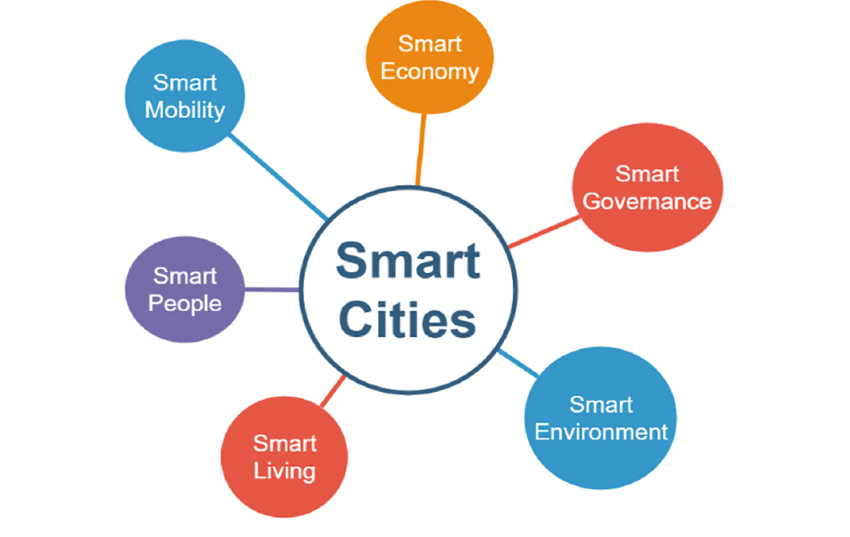
\includegraphics[width=0.7\columnwidth]{images/The-six-pillars-of-Smart-Cities-based-on-8.png}
\caption{The six pillars of Smart Cities \cite{foo3}}
\end{figure}


% Cambiare la forma per evitare l'accapo dell'elenco puntato - FATTO
    

    
 
In a \textbf{Smart Economy}, the focus is on fostering creativity and encouraging entrepreneurial endeavors. This entails cultivating a culture that values \textbf{innovation} and actively supports the initiation of new businesses. The objective is to establish a distinct economic identity through a proactive approach to building trademarks, attracting investments, and gaining global recognition.
Emphasis is placed on optimizing productivity through advanced technologies and adaptable work structures. The labor market's \textbf{flexibility} becomes crucial for resilience in the face of changing economic landscapes. Moreover, active engagement on the international stage is a priority, with a commitment to open trade, collaboration, and continuous transformation for sustained economic growth.

 
The spotlight in a so-defined \textbf{Smart Governance} is on \textbf{citizen participation} in decision-making processes. This involves ensuring that the public is not merely the recipient of policies but an active contributor to shaping them. \textbf{Services} provided by the government, both public and social, are streamlined for efficiency, with a transparent governance structure ensuring accountability and trust.
The long-term vision in political strategies becomes paramount, focusing on sustainability and the well-being of future generations. Smart Governance is characterized by its \textbf{forward-thinking approach}, responsive nature, and a commitment to serving the collective interest of the citizens.


  In a society embracing the principles of \textbf{Smart People}, the primary focus is on education and continuous skill development. The population's high level of qualification becomes the bedrock of innovation and productivity. Lifelong learning is not just encouraged but ingrained as a cultural norm, ensuring \textbf{adaptability to technological advancements}. Diversity, both social and ethnic, is actively celebrated, fostering an environment that values flexibility and creativity. A Smart People society places a premium on a global perspective, encouraging cosmopolitanism and open-mindedness. \textbf{Active participation} in public life is promoted to enhance civic engagement.

    
  \textbf{Smart Mobility} centers around the integration of efficient and interconnected transportation systems. Local accessibility is prioritized through well-connected public transportation, reducing reliance on individual vehicles and contributing to sustainable urban living. International accessibility is also emphasized to enhance cultural exchange and economic activities.
The availability of advanced Information and Communication Technology (ICT) infrastructure is foundational for Smart Mobility. \textbf{Real-time information} empowers individuals to make \textbf{informed transportation choices}, contributing to the reliability and efficiency of transportation networks. \textbf{Sustainability} is a key principle, with a focus on innovative, safe, and eco-friendly transport systems.

 
In a \textbf{Smart environment} the goal is to balance the appeal of natural conditions with responsible environmental practices. \textbf{Pollution control measures} are prioritized, encompassing stringent regulations and sustainable practices to safeguard air, water, and soil quality.
Environmental protection extends beyond national boundaries, with active participation in international efforts to address climate change and protect biodiversity. \textbf{Sustainable resource management} is fundamental, ensuring responsible usage and conservation of natural resources for the benefit of current and future generations. The overarching aim is to integrate environmental sustainability into various societal aspects for a harmonious balance.
    
  \textbf{Smart Living} embraces a holistic approach to improving the quality of life. Cultural facilities, health conditions, individual safety, housing quality, education facilities, touristic attractiveness, and social cohesion collectively contribute to an environment that prioritizes the well-being of its inhabitants.
This involves the development of cultural spaces, accessible healthcare systems, secure living ..environments, high-quality housing, robust educational systems, and an inviting atmosphere for visitors. Social cohesion initiatives strengthen the community fabric, fostering a sense of belonging and support.


These domains serve as the foundational pillars of smart cities, and any undertaking focused on their advancement should encompass one or more of these pillars. Additionally, it is crucial to acknowledge the \textbf{interconnection} between them, ensuring that progress in one area does not adversely impact another. 

\subsection{Real examples of Smart City}
\label{subsec:ExamplesOfSmartCities}
After defining the concept of a Smart City and outlining its key pillars, let's explore three widely recognized examples of smart cities, highlighting the factors that make them exemplary models to emulate \cite{foo4}.

% Cambiare a \subsubsection o \paragraph -- CAMBIATO IN SUBSUBSECTION

\subsubsection{Singapore}
Global smart city trailblazer, Singapore is a living laboratory for cutting-edge technologies. In digital health, it uses AI for skin cancer detection, radiographic diagnosis, and diabetic identification, reducing hospital stays. Its urban mobility revolution includes a communication-centric traffic management strategy with autonomous vehicles and vehicle-to-everything systems.
Intelligent finance is another focus, with AI integrated into banking and insurance systems for tasks like facial recognition, smart contracts, and subscription renewals. The retail sector uses AI algorithms for a customer-centric approach, guiding customers to relevant products. In education, robotics and algorithmics are integrated, with humanoid robots supporting or replacing teachers in lower-grade levels.
The "Virtual Singapore" project \cite{VirtualSingapore}, a 3D virtual map of the city's infrastructure, allows for sophisticated simulations optimizing energy, environment, and economics choices. Risk simulation using this model aids in disaster management planning. Future projects include drone highways and virtual reality tourism experiences.
Healthcare accessibility improvements include autonomous wheelchairs for the elderly, moving towards a city with barrier-free architecture and reliable traffic management. Advanced digital identity systems like SingPass provide access to administrative services, banks, and healthcare data, with ongoing developments in payment methods for tolls, veterinary care identification, state assistance allocation, and emergency communication platforms. This holistic approach showcases Singapore's dedication to creating a seamlessly interconnected ecosystem for its residents, establishing it as a \textbf{paradigm} for the future of urban living.

\subsubsection{Seoul} 
The capital of South Korea is a prominent global tech hub and tourist destination \cite{Hwang2013}. The Smart Seoul initiative, launched in 2015, builds on the u-City project to enhance sustainability, competitiveness, and citizen well-being through smart technologies. The initiative focuses on three key aspects: robust ICT infrastructure, an integrated city-management framework, and smart users. Utilizing ICT tools, the city engages citizens in developing and using smart services.
Safety services, like u-Seoul Safety Service, employ location-based and CCTV technologies to address emergencies, prioritizing vulnerable groups. The U-Children Safety System enhances child safety through wireless networks, reflecting the city's commitment to inclusivity. A network of smart device users, supported by broadband and wireless networks, empowers citizens. Smart device accessibility is extended through education programs targeting diverse demographics.
The u-Seoul Net, a comprehensive communication network completed in 2011, provides free Wi-Fi access and administrative services, contributing to smart infrastructure. Open data is a cornerstone of Seoul's smart city development, exemplified by the Seoul Open Data Square \cite{SeoulOpenData} launched in 2012. This initiative offers transparent access to diverse public information, fostering innovation and collaboration. Inclusivity is a key focus, engaging citizens in developing and improving smart services. The open data approach aligns with Smart Seoul's broader vision, ensuring technological advancements benefit the entire community and contribute to overall well-being.


\subsubsection{Milan} 
The city strategically positions itself as a leader in the smart city landscape, prioritizing electric mobility, cutting-edge technology, and digital initiatives, as evidenced by the "Booklet Smart City 2023" report \cite{SmartCity2023}. Notable achievements include successful waste separation, increased adoption of low-emission vehicles, and efficient public lighting systems, highlighting the city's commitment to sustainability. However, challenges such as air quality issues and water losses persist.
In terms of digital infrastructure, Milan excels with 100\% broadband coverage and widespread public Wi-Fi. The city actively integrates sensor devices for enhanced data collection and analysis. Sustainable mobility initiatives showcase Milan's leadership, with a 12.6\% increase in low-emission vehicle adoption in 2021, robust electric vehicle charging stations, and sharing mobility services. Challenges include air quality concerns and deficits in green spaces.
Despite challenges, Milan achieves a noteworthy 62.5\% recycling rate and implements district heating networks and active solar panels. The city addresses challenges by embracing smart working trends, with 64\% of companies offering smart working options. Milan's digital transformation extends to city services, emphasizing online administrative and informational services. Citizen engagement is fostered through digital platforms, notably the advanced e-welfare platform WeMi \cite{WeMiWebsite}, aggregating welfare services from the City of Milan and selected entities.
In summary, Milan actively steers towards becoming a smarter city, balancing achievements with challenges. Its dedication to sustainability, technological advancements, and digital innovation reflects its commitment to creating a resilient and vibrant urban environment.\\

A pivotal element in the evolution towards a Smart City is the embrace of information liberalization, as exemplified by Seoul through the establishment of Open Data portals. These platforms facilitate the accessibility of diverse datasets to the public. Leveraging this data, individuals, businesses, and organizations can embark on a multitude of projects, fostering the well-being and advancement of the city.

\section{Open Data in Smart Cities}

Open data is, by definition \cite{dataEuropa} data "\textit{that refers to the information collected, produced or paid for by the public bodies (also referred to as Public Sector Information) and made freely available for re-use for any purpose}".

In recent years, the rapid advancement of technologies like the \textbf{IoT} (Internet of Things) and analytics, coupled with the continuous expansion of data volume (commonly referred to as big data), has fueled a vision where data and technology collaboratively contribute to enhancing the quality of life for both citizens and businesses in urban environments. The assertion is that cloud-based data and technology play a pivotal role in enabling \textbf{real-time, data-driven decision-making} processes that lead to improved urban management. Furthermore, the development of a smart city initiative is now intricately linked to factors such as connectivity, \textbf{open data practices}, and the widespread use of sensors. The type of data collected varies widely, encompassing aspects ranging from health services to governmental measures, social dynamics, economic indicators, and environmental impacts. Traditionally, public organizations have collected, managed, and processed data for internal purposes. However, the emergence of the open data movement in the past decade has prompted these organizations to share their data publicly, contributing to a \textbf{more transparent and accessible} data landscape.
In today's smart city ecosystem, a plethora of \textbf{sensors}, along with various tools and technologies such as cameras, kiosks, personal devices, appliances, and social networks, contribute to the extensive collection of data. This data collection serves as a valuable tool for both citizens and urban planners, facilitating better control and access to necessary information.
\begin{figure}
\centering
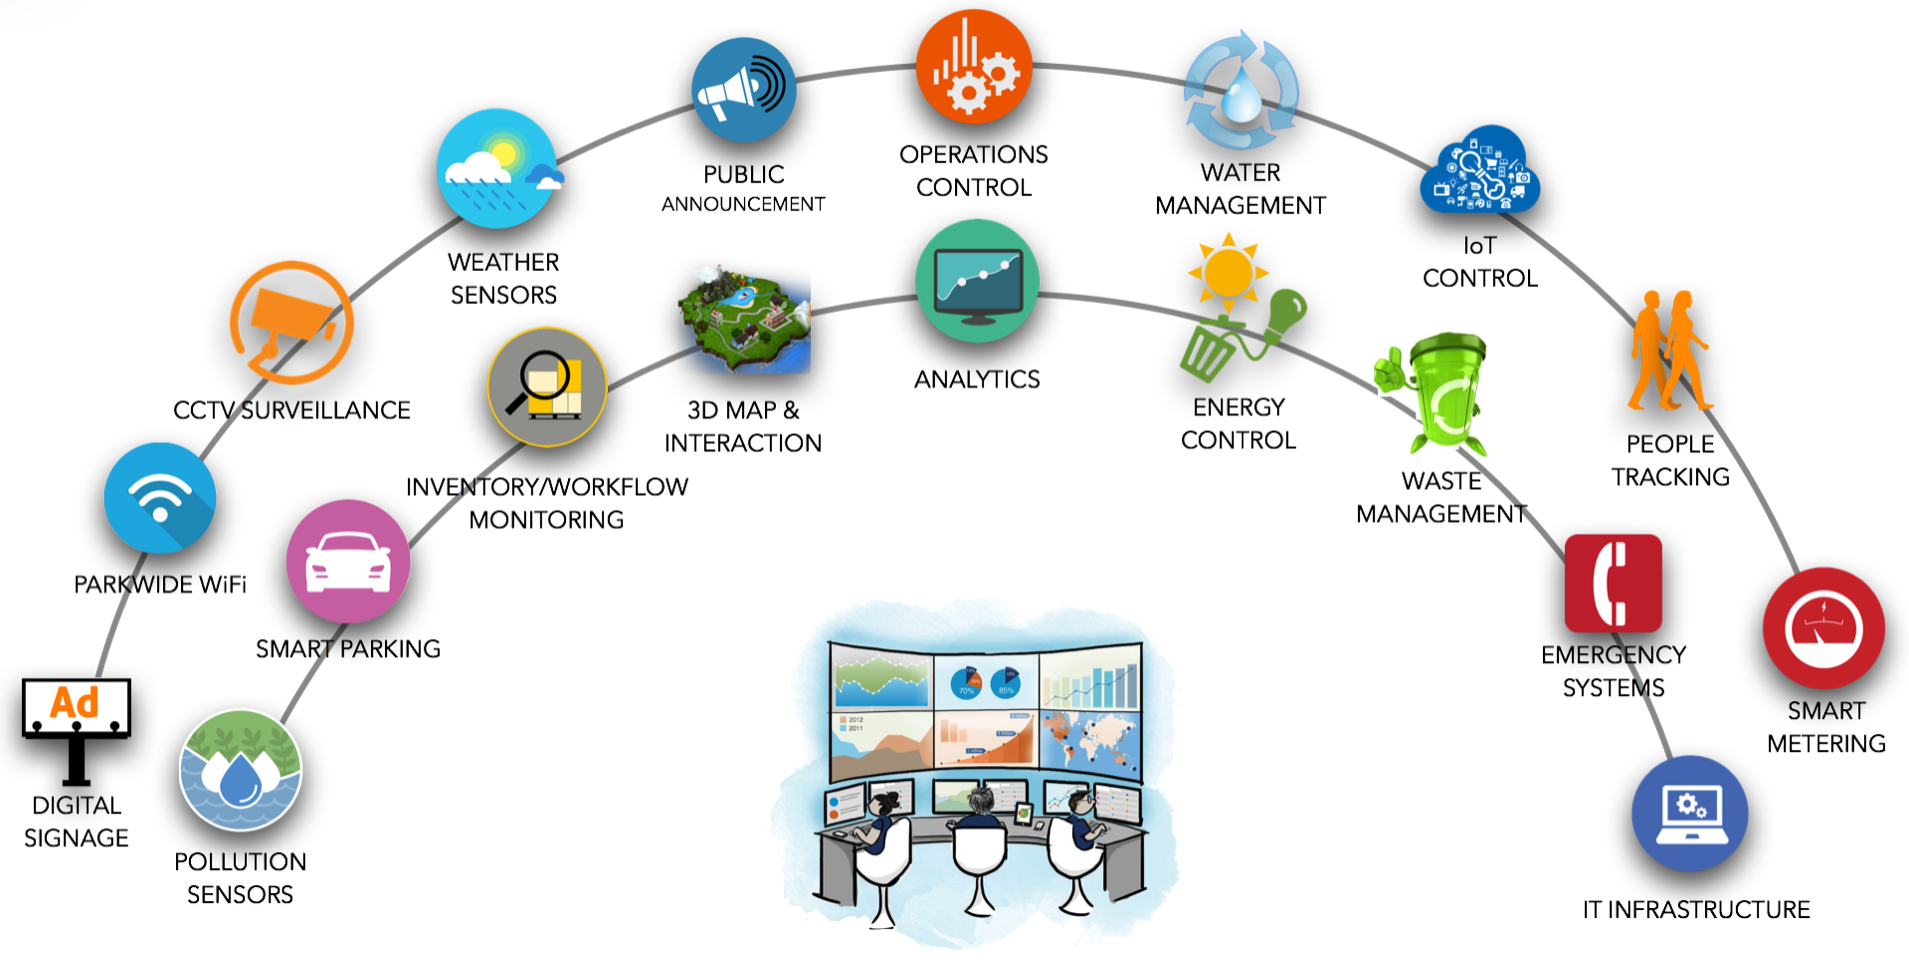
\includegraphics[width=0.9\columnwidth]{images/SmartCity.png}
\caption{Sources of data for smart city management \cite{figureSourcesofData}}
\end{figure}
The term "open data" is not confined to government data alone; it extends to the private sector, where recognition of the potential benefits of sharing data is growing. Both public and private entities now acknowledge the value of data as a key resource that enhances efficiency and effectiveness in various everyday activities. In the context of smart cities, the number and diversity of stakeholders involved are notably higher than in traditional private business cases. This includes utility companies, transport providers, mobile phone operators, social media platforms, financial institutions, surveillance and security providers, emergency services, and, notably, the citizens themselves. The collective appreciation of the value of data underscores its central role in shaping the present and future of smart urban environments.

\subsection{International Collaboration: Open Data and Sustainable Development Goals}
Open Data initiatives are also promoted by governative organizations, such as EU, giving the members a Directive (2019/1024)\cite{EU2019Directive}, based on the general principle that public data and data funded with public funds should be reusable for commercial or non-commercial purposes. The directive promotes the use of open data presented in open formats that can be freely used and shared for any purpose.

\begin{itemize}
    \item \textbf{Format and Accessibility}: Public entities and public enterprises must make documents available in any language or pre-existing format. Electronic availability through open, machine-readable, accessible, searchable, and reusable formats, along with metadata, is encouraged.
    \item \textbf{Practical Provisions for Reuse}: Public entities must examine reuse requests, making documents available electronically within a reasonable timeframe. Measures to facilitate online search and retrieval of documents are required.
    \item \textbf{Dynamic and Real-time Data}: Dynamic data must be immediately available through application programming interfaces (APIs) and, if necessary, as bulk downloads.
    \item \textbf{Research Data}: Member States must adopt national policies to open up publicly funded research data following the FAIR\footnote{FAIR data are data which meet principles of findability, accessibility, interoperability, and reusability (FAIR).} principles, considering intellectual property rights, personal data protection, privacy, security, and legitimate commercial interests.
    \item \textbf{Non-Discrimination and Transaction Equity}: Reuse of documents is open to all market actors without discrimination. Exclusive rights in contracts between public entities or public enterprises and third parties are generally discouraged, and specific transparency requirements apply to allowable agreements.

    \item \textbf{High-Value Data Sets}: Documents associated with significant socioeconomic benefits should be made available under particularly favorable reuse conditions. The directive mandates the European Commission to adopt a list of high-value data sets, covering six thematic categories (geospatial, earth and environment observation, weather, demographic, mobility, business and company ownership data).
\end{itemize}

Moreover, open data plays a crucial role in advancing the global pursuit of sustainable development, aligning closely with the United Nations Sustainable Development Goals (SDGs)\cite{sdgs}. By fostering transparency, \textbf{collaboration}, and innovation, open data emerges as a powerful catalyst for addressing the complex challenges outlined by the SDGs. It transcends borders, providing a shared resource that empowers individuals, communities, and nations to collectively work towards a more sustainable and equitable future. The inherent openness of data facilitates a deeper understanding of societal issues, allowing stakeholders to make informed decisions and implement effective solutions. This transparency promotes accountability among governments, encourages citizen engagement, and contributes to the common goal of creating inclusive and fair societies. Moreover, the accessibility of data enables the identification of gaps and disparities, facilitating targeted interventions to uplift marginalized communities and bridge socioeconomic divides. Furthermore, open data fosters collaboration on a global scale. By breaking down barriers and facilitating the exchange of information, it enables nations to learn from each other's successes and challenges. This collaborative approach is essential for tackling transboundary issues such as climate change, poverty, and health crises, which are central to the SDGs. Open data can become a unifying force that empowers nations to collectively address shared challenges and work towards common objectives.

\subsection{Application examples of Open Data}

In the realm of real-world application of open data, a myriad of applications have emerged, showcasing the transformative power of data-driven solutions across diverse domains. Let's explore seven examples of applications that highlight the versatility of open data in addressing real-world challenges.
In the realm of real-world application of open data, a myriad of applications have emerged, showcasing the transformative power of data-driven solutions across diverse domains. Let's explore seven examples of applications that highlight the versatility of open data in addressing real-world challenges \cite{electronics10232997}.
\begin{enumerate}
\item \textbf{Air Quality Monitoring Systems:}
   Numerous cities have embraced open data to develop low-cost air pollution monitoring systems. By integrating data from various sources, such as sensors scattered around the city, these systems enable real-time tracking of air quality indices in each area, helping authorities and citizens make informed decisions about outdoor activities and health precautions.

\item \textbf{Traffic Flow Optimization:}
   Leveraging open data on traffic patterns and atmospheric conditions, smart city initiatives aim to optimize traffic flow. By employing machine learning algorithms, these projects forecast congestion-prone areas, facilitating dynamic traffic signal control, as we have seen in the Singapore example. The goal is not only to reduce travel time but also to minimize vehicular emissions and alleviate pollution.

\item \textbf{Urban Green Spaces Mapping:}
   Open data plays a crucial role in mapping and monitoring urban green spaces. By utilizing satellite imagery and geospatial data, projects identify areas with vegetation cover, helping city planners enhance green infrastructure. This, in turn, contributes to improved air quality and overall environmental well-being.

\item \textbf{Water Resource Management:}
   Machine learning algorithms applied to open data sets can extract valuable insights for water resource management. By analyzing satellite images and GIS data, projects identify non-water bodies like urban areas and vegetation. This aids in efficient water resource management, preventing contamination and ensuring sustainable use.

\item \textbf{Accident Prediction Models:}
   Open datasets of large cities are harnessed to create high-resolution accident prediction models. Machine learning methods are employed to predict accident-prone zones, contributing to proactive measures for improving road safety.
   
\item \textbf{Flood Monitoring and Prediction:}
   Open data, including weather information and satellite imagery, is utilized to develop flood monitoring and prediction systems. Machine learning models can effectively classify images related to drain blockages and abnormal water levels, assisting in early detection and response to potential flooding events.

\item \textbf{Urban Energy Consumption Modeling:}
   Utilizing open data, particularly smart metering information and building footprints, projects develop models for predicting urban energy consumption. Machine learning algorithms enable accurate forecasting of energy demand, aiding in the implementation of energy-efficient practices and reducing the environmental footprint of urban areas.
\end{enumerate}

These real-world projects demonstrate the impactful synergy between open data and innovative technologies, addressing several challenges related to urbanization and pollution.

\section{Pollution monitoring in smart cities}

As mentioned above, one of the critical challenges lies in effectively build an air quality management system. This system plays a pivotal role in detecting hazardous gases, enabling residents to make informed decisions about their living spaces. Additionally, it serves as a catalyst for governmental interventions aimed at reducing the sources of these harmful emissions.

The traditional notion of literature often depicted industrial zones as having precarious air quality, while green areas were considered healthier. However, in contemporary times, this paradigm has shifted, and even green spaces are not exempt from air quality concerns \cite{rhaiemair}. Clean and fresh air is a fundamental element for a healthy life, but numerous factors impact its purity.

Air pollution emerges as a critical health issue in cities, causing significant premature deaths globally. The World Health Organization (WHO) reports that outdoor Ambient (outdoor) air pollution is estimated to have caused 4.2 million premature deaths worldwide in 2019 \cite{WHO2018AirPollution}. Urban areas grapple with air pollution, with a particular focus on Particulate Matter (PM), especially PM 2.5 and PM 10, which can penetrate the respiratory system.

To address these challenges, smart cities must prioritize the monitoring of environmental conditions. Deploying a network of low-cost air quality monitoring sensor nodes becomes essential to identify pollution sources and mitigate their impact. By detecting sources of pollution, cities can take corrective actions, enhancing environmental health. Implementing disaster detection systems, such as flood and precipitation monitoring solutions, provides citizens with advanced warnings. This holistic approach allows authorities to make informed, data-driven decisions for infrastructure planning and policy formulation. Continuous study of air quality variables is crucial to effectively classify cities based on the safety and well-being of their residents.

\subsection{Main pollutants in urban spaces}

In air quality studies, some pollutants emerge as more impactful on public health, making them a threat to keep an eye on. Here are six of them:
\begin{itemize}
    \item \textbf{Ozone (O\textsubscript{3})}: this gas poses, especially on hot days, health risks by causing respiratory issues such as coughing, difficulty breathing, and lung inflammation.
    \item \textbf{Nitrogen dioxide (NO\textsubscript{2})}: mainly emitted from fuel combustion, irritates human airways and can worsen respiratory conditions, especially asthma, causing short-term exacerbations and respiratory symptoms.
    \item \textbf{Solfure dioxide (SO\textsubscript{2})}: subproduct of fuel combustion in various sources, irritates eyes and the respiratory system. Low concentrations affect the eyes and upper respiratory tract, while higher levels can lead to nasal irritation, bronchitis, and lung disease.
    \item \textbf{Carbon monoxide (CO)}: this pollutant derives from fossil fuels, common in traffic, harms cardiovascular health, causing issues for individuals with heart disease and affecting anyone with vision and cognitive problems at high levels, potentially leading to fatalities.
    \item \textbf{Fine particulate matter (PM\textsubscript{2.5})}: tiny airborne particles from various sources, can enter the respiratory system and bloodstream, leading to health issues such as respiratory and cardiovascular problems.
    \item \textbf{Particulate matter (PM\textsubscript{10})}: larger than PM\textsubscript{2.5} particles, includes various sources like combustion and industrial processes. While primarily affecting the upper respiratory tract, PM\textsubscript{10} poses health risks, especially for those with respiratory conditions. 
\end{itemize}


In brief, the discussed urban pollutants can significantly impact public health and well-being. The widely used measure to assess overall air quality, is the Air Quality Index (AQI), which provides a comprehensive score that helps the public grasp the current state of the air they breathe.

\subsection{The Air Quality Index}

The computation of the Air Quality Index (AQI) relies on the measurement of air pollutant concentrations over specific time intervals, obtained from air monitors or models. The combination of concentration and time represents the dose of the air pollutant. The health effects associated with pollutants are determined through epidemiological research. It is important to note that different pollutants have varying impacts, and the conversion function from concentration to AQI is different for each pollutant. AQI values are categorized into ranges, each associated with a descriptor, color code, and standardized public health advisory.
On days when the AQI is predicted to be elevated due to fine particle pollution, agencies or public health organizations may take several measures:
\begin{compactenum}
    \item Advise sensitive groups, such as the elderly, children, and individuals with respiratory or cardiovascular issues, to avoid outdoor exertion.
    \item Declare an "action day" to encourage voluntary measures, such as using public transportation, to reduce air emissions.
    \item Recommend the use of masks outdoors and air purifiers indoors to prevent fine particles from entering the lungs.
\end{compactenum}
In cases of very poor air quality, such as during air pollution episodes, when the AQI indicates a potential for significant harm to public health from acute exposure, agencies may implement emergency plans. These plans can include orders for major emitters, like coal-burning industries, to curtail emissions until hazardous conditions improve.
It's important to note that not all air contaminants have an associated AQI. Many countries monitor pollutants such as ground-level ozone, particulates, sulfur dioxide, carbon monoxide, and nitrogen dioxide, calculating air quality indices for these substances.
There is also a website \cite{Airqualityindexwebsite} that allows government agencies worldwide to submit real-time air monitoring data. This platform employs a common definition of the air quality index, facilitating a standardized display of information.

Each country sets its air quality index thresholds based on factors such as territorial morphology. In the European Union (EU), specific values have been established, ranging from 1 (good) to 6 (extremely poor), as depicted in the table \ref{fig:euaqitable}. The index for each pollutant is determined independently based on concentrations, with higher concentrations corresponding to higher index values. The European Air Quality index for a specific hour is simply the highest value among the five individual pollutant indexes calculated during that hour. Similarly, the daily European Air Quality index is the highest value of the overall hourly index for the corresponding day.
\begin{figure}
    \centering
    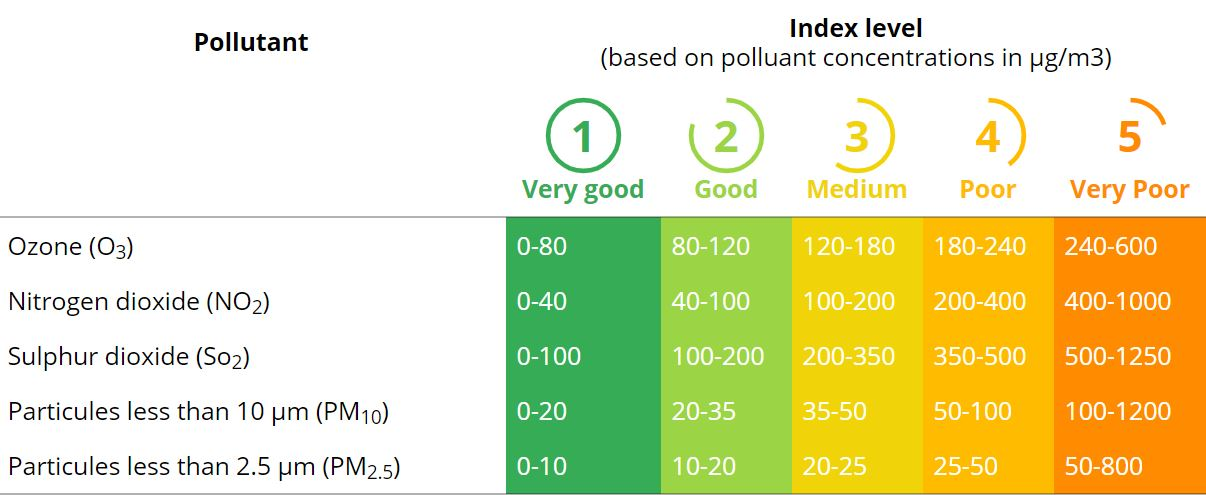
\includegraphics[width=1\linewidth]{images/airqualityindexcalc.png}
    \caption{European air quality index thresholds}
    \label{fig:euaqitable}
\end{figure}

As we can see, Europe does not take into account the measurements of CO concentration for the calculation of the Index.

\subsection{Beijing example}

In 1998, Beijing initiated a concerted effort to address air pollution, acknowledging the environmental issues confronting one of the world's largest and fastest-growing cities. Initially grappling with pollution driven by coal combustion and vehicular emissions, surpassing national limits, the city undertook a series of measures over the subsequent 15 years. These efforts aimed at optimizing energy infrastructure, controlling coal-fired pollution, and regulating vehicle emissions. By 2013, significant reductions in air pollutants were evident, meeting national standards for specific pollutants \cite{CCAC2019}.
However, the pivotal moment materialized in 2013, marked by Beijing adopting more systematic and intensive measures for air pollution control. By the close of 2017, there was a notable 35\% decrease in fine particulate pollution (PM\textsubscript{2.5}). This achievement resulted from targeted actions like controlling coal-fired boilers, advocating for cleaner domestic fuels, and restructuring industries. During this timeframe, emissions of sulfur dioxide (SO\textsubscript{2}), nitrogen oxides (NO\textsubscript{x}), particulate matter (PM\textsubscript{10}), and volatile organic compounds in Beijing saw a substantial decrease. Beijing's approach to air quality management distinguishes itself with robust monitoring, pollution source identification, emission inventories, comprehensive legal standards, and stringent environmental law enforcement. 

\begin{figure}
    \centering
    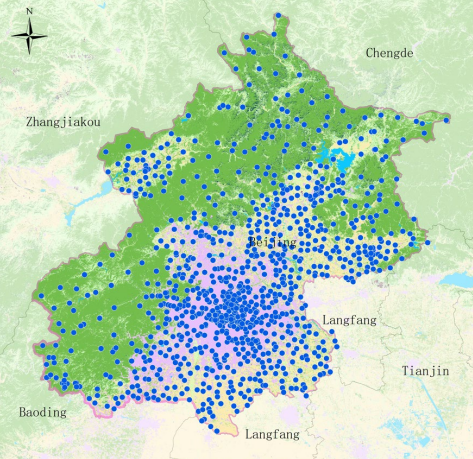
\includegraphics[width=0.5\linewidth]{images/beijingsensors.png}
    \caption{Beijing's high-density sensor-based PM\textsubscript{2.5} monitoring network \cite{UNEnvironment2019}}
    \label{fig:beijingsensors}
\end{figure}

Despite recognizing achievements, the Beijing municipality acknowledges persistent challenges, particularly concerning PM\textsubscript{2.5} concentrations that still fall short of national standards, and because episodes of heavy pollution persist during autumn and winter. Nevertheless, Beijing affirms its commitment to sharing accumulated knowledge and experiences on air pollution with other developing cities, emphasizing that addressing air quality issues is an ongoing and long-term process.

\paragraph{}

In this work the air quality prediction task is explored using deep learning models. We aim to find patterns in air pollutant data to develop more effective strategies for mitigating the impact of pollution on public health. By comparing different deep learning approaches, the research aims to identify the most reliable methods for forecasting pollutant concentrations, providing valuable insights for informed decision-making and targeted governmental interventions.

\section{Previous works on air pollutants forecasting}
\label{cap1:sota}
Over the years, numerous authors have endeavored to address the challenge of predicting pollutants in cities using various methods, encompassing both classical and deep learning techniques. The primary obstacles encountered in this task include:

\begin{enumerate}
  \item \textbf{Missing Data}, arising from erroneous observations or sensor unavailability.
  \item \textbf{Collinearity} between the target variables.
  \item \textbf{Complex and Multiple Seasonality Patterns}, which adds another layer of complexity.
\end{enumerate}

The models employed must demonstrate proficiency in learning from extended sequences to make accurate forecasts. Additionally, they should incorporate mechanisms that facilitate the interaction among features for enhanced predictive capabilities.

\textbf{Classical models}, like ARIMA (referenced in \cite{DIAZROBLES20088331} and \cite{Jodar2013}), have demonstrated the ability to predict the overall trend of time series data. However, they often fall short in predicting peaks, possibly due to their inability to capture the nonlinear patterns typically present in air quality time series. Moreover, the datasets used in these analyses focused on univariate regression problems, predicting each pollutant individually. To address these limitations, the papers suggest an innovative approach: combining an artificial neural network architecture with the ARIMA model. Additionally, meteorological variables are incorporated as external regressors to enhance predictive accuracy.\\

With increased computing capacity and rapid growth in deep learning studies, the development of \textbf{more sophisticated network architectures} has become possible. These architectures can capture complex patterns and combine spatial and temporal features of this kind of data.
Many approaches include the use of \textbf{Long-Short Term Memory (LSTM) networks}, combined with various mathematical and statistical techniques.

\noindent K\"{o}k et al. \cite{8258144} use a simple LSTM to make one-step-ahead predictions of Ozone and NO\textsubscript{2}. Then the predictions are used to classify the AQI for the predicted day.

\noindent Han et al. \cite{9127775} proposed a combination of Bayesian, domain-specific knowledge, and deep learning to reduce error. The approach enables the fusion of different forecast strategies thanks to probabilistic Bayesian modeling, reducing overfitting and providing a measure of uncertainty.

\noindent Song et al. \cite{lstmkalman} introduced a time prediction model, LSTM-Kalman, for forecasting time series data with long-term and short-term characteristics. Leveraging LSTM's memory feature, the model captures and stores information from previous data, utilizing it in subsequent processing to obtain the underlying time series. Kalman filtering is used to dynamically adjusts the LSTM-processed data sequence, yielding an improved predicted value.

\noindent Yin et al. \cite{Yin2020} presented DAEDN (Denoising Auto Encoder Deep Network), a novel air pollutant prediction model based on bidirectional LSTM networks. Trained on 5 years of Beijing's PM\textsubscript{2.5} data, DAEDN outperforms unidirectional LSTM with a 7.33\% reduction in RMSE and a 5.87\% reduction in MAE. The model effectively extracts stable features from noisy input, considering time series properties and integrating environmental big data sources such as weather data.

\noindent Jin et al. \cite{WaveletNLSTM} suggested a neural network architecture for multivariate, multi-step predictions using Wavelet transform to decompose the time series of pollutants. They then input the components into a Nested-LSTM layer, allowing an extension of the memory capability of the traditional LSTM, and combine the features obtained from each layer in a shared layer before the output layer.

\noindent Similarly, Zeng et al. \cite{ZENG2022108822} proposed a model that integrates the extended stationary wavelet transform (ESWT) and the nested long short-term memory (NLSTM) neural network for PM\textsubscript{2.5} forecasting. The authors claim that the method outperforms state-of-the-art forecasting methods in terms of different error metrics, such as absolute error, R2, MAE, RMSE, and MAPE.\\


In the last four years, as the availability of data increased, new approaches taking into account the \textbf{spatial information} of the data, obtained by multiple stations observing at the same time, occurred:

\noindent Qi et al. \cite{graphlstm1}, proposed a hybrid model for spatiotemporal forecasting of PM\textsubscript{2.5} based on graph convolutional neural network and LSTM, which applies a Graph Convolutional Network (GCN) to extract the spatial dependence between different stations and LSTM to capture the time dependence between observations at different times. 

\noindent Wen et al. \cite{WEN20191091} suggested a Convolutional Long Short-Term Memory Neural Network Extended (C-LSTME), designed for predicting air quality concentration. To effectively capture both spatial and temporal aspects of the data, the model incorporates historical air pollutant concentrations from the current station, as well as those from adaptively selected k-nearest neighboring stations. The integration of Convolutional Neural Network (CNN) and LSTMs facilitates the extraction of high-level spatiotemporal features. Additionally, the model incorporates meteorological and aerosol data after the feature extraction before a multilayer perceptron (MLP) block, to enhance its predictive performance.

\noindent Wang and Han \cite{Wang2023} proposed a Dirichlet Graph Convolution Coupled Neural Differential Equation for Spatio-temporal Time Series Prediction. This GCCNDE model predicts by learning initial spatio-temporal features, mapping them to a high-dimensional space, modeling dynamic evolution with GAT and NDE, and obtaining final predictions by mapping the high-dimensional state back to the original space. It assumes shared spatial representations between adjacent time steps for effective prediction.

In this work, various model architectures for a multivariate multi-step forecasting has been tested, using both external features and historical values. In the next chapter a deep analysis of three air quality datasets will be conducted.
\newpage



















\chapter{Datasets inspection}
\label{chap:Datasets}

In the context of the conducted research, the selection and analysis of datasets play a fundamental role in understanding and addressing the challenges presented in this task. This chapter delves into the datasets chosen as the foundation for investigations, as these data serve as the raw material from which crucial information is extracted for analysis. By systematically considering the origins, dimensions, and peculiarities of these datasets, we can establish a foundation for comprehending the dynamics that define this field of study.
As mentioned in the previous chapter, one of the main challenges in analyzing pollution data is the presence of erroneous or missing data, often caused by faulty or dirty sensors. 
It is important to consider outliers, as they may represent either actual observations of a significant increase in pollutants or random errors in the sensor. The location of the sensor is also a crucial factor that can affect the average values of the series. 
To account for this variability in the data based on location, three datasets have been selected for analysis, namely:
\begin{itemize}[noitemsep]
    \item Citypulse (containing data from Aarhus, Denmark),
    \item Seoul pollution data,
    \item Madrid pollution data.
\end{itemize}

These three cities are located in three different regions, each with its own unique lifestyle, morphology, and climate.

\section{Data availabilty}
\subsection{Citypulse}
Created in the context of the CityPulse EU FP7 Project, this collection of datasets contains a lot of annotated data, relevant in the context of a smart city \cite{CityPulseDataset}. For this analysis, the following datasets have been chosen:
\begin{itemize}[noitemsep]
    \item \textbf{Pollution data}
    \item Road traffic data
    \item Weather data
    \item Parking data
\end{itemize}

It is highlighted in the website that while the other three datasets are provided as observations from real sensors, the pollution dataset is generated using a simple function that uses controlled randomness to provide a realistic and bounded measurement\footnote{The stream generation for sensor measurements involves updating values every 5 minutes. If the initial value is below 20, it increases by a random integer between 1 and 10. If the value exceeds 210, it decreases by a random integer between 1 and 10. Otherwise, it changes by a random integer between -5 and 5 to create a realistic and bounded measurement stream.}. To avoid using this generated data, which would likely bias the results of our prediction algorithms, actual values of the available pollutants are extracted from another source \cite{EEA_AirQuality}.
The dataset spans from August 2014 to October 2014 and contains a total of 10,560 observations. Each observation is recorded at regular intervals of 5 minutes. However, for the purpose of this analysis, we resample the data on an hourly basis. 
Missing data in the time series are imputed via linear interpolation, as most of the variables did not have long series of consecutive missing data.

\begin{table}[h]
\centering
\begin{tabular}{|c|c|}
\hline
\textbf{Category} & \textbf{Variables} \\ \hline
Air Pollution Observations & \begin{tabular}[c]{@{}c@{}}O\textsubscript{3}, PM\textsubscript{10}, \\PM\textsubscript{2.5}, NO\textsubscript{2}\end{tabular} \\ \hline
Meteorological Data & \begin{tabular}[c]{@{}c@{}}temp, feelslike, humidity, precip,\\ precipprob, windspeed, cloudcover, visibility\end{tabular} \\ \hline
Traffic and Parking Data & \begin{tabular}[c]{@{}c@{}}vehicleCount, avgSpeed, \\ Totalspaces,occupied, occupancy\end{tabular} \\ \hline
\end{tabular}
\caption{Variables in the CityPulse Dataset. Description of each variable is found on Table \ref{apptable:Citypulse_variable_descriptio} in the appendix.}
\end{table}

\newpage

\begin{figure}[h]
    \centering
    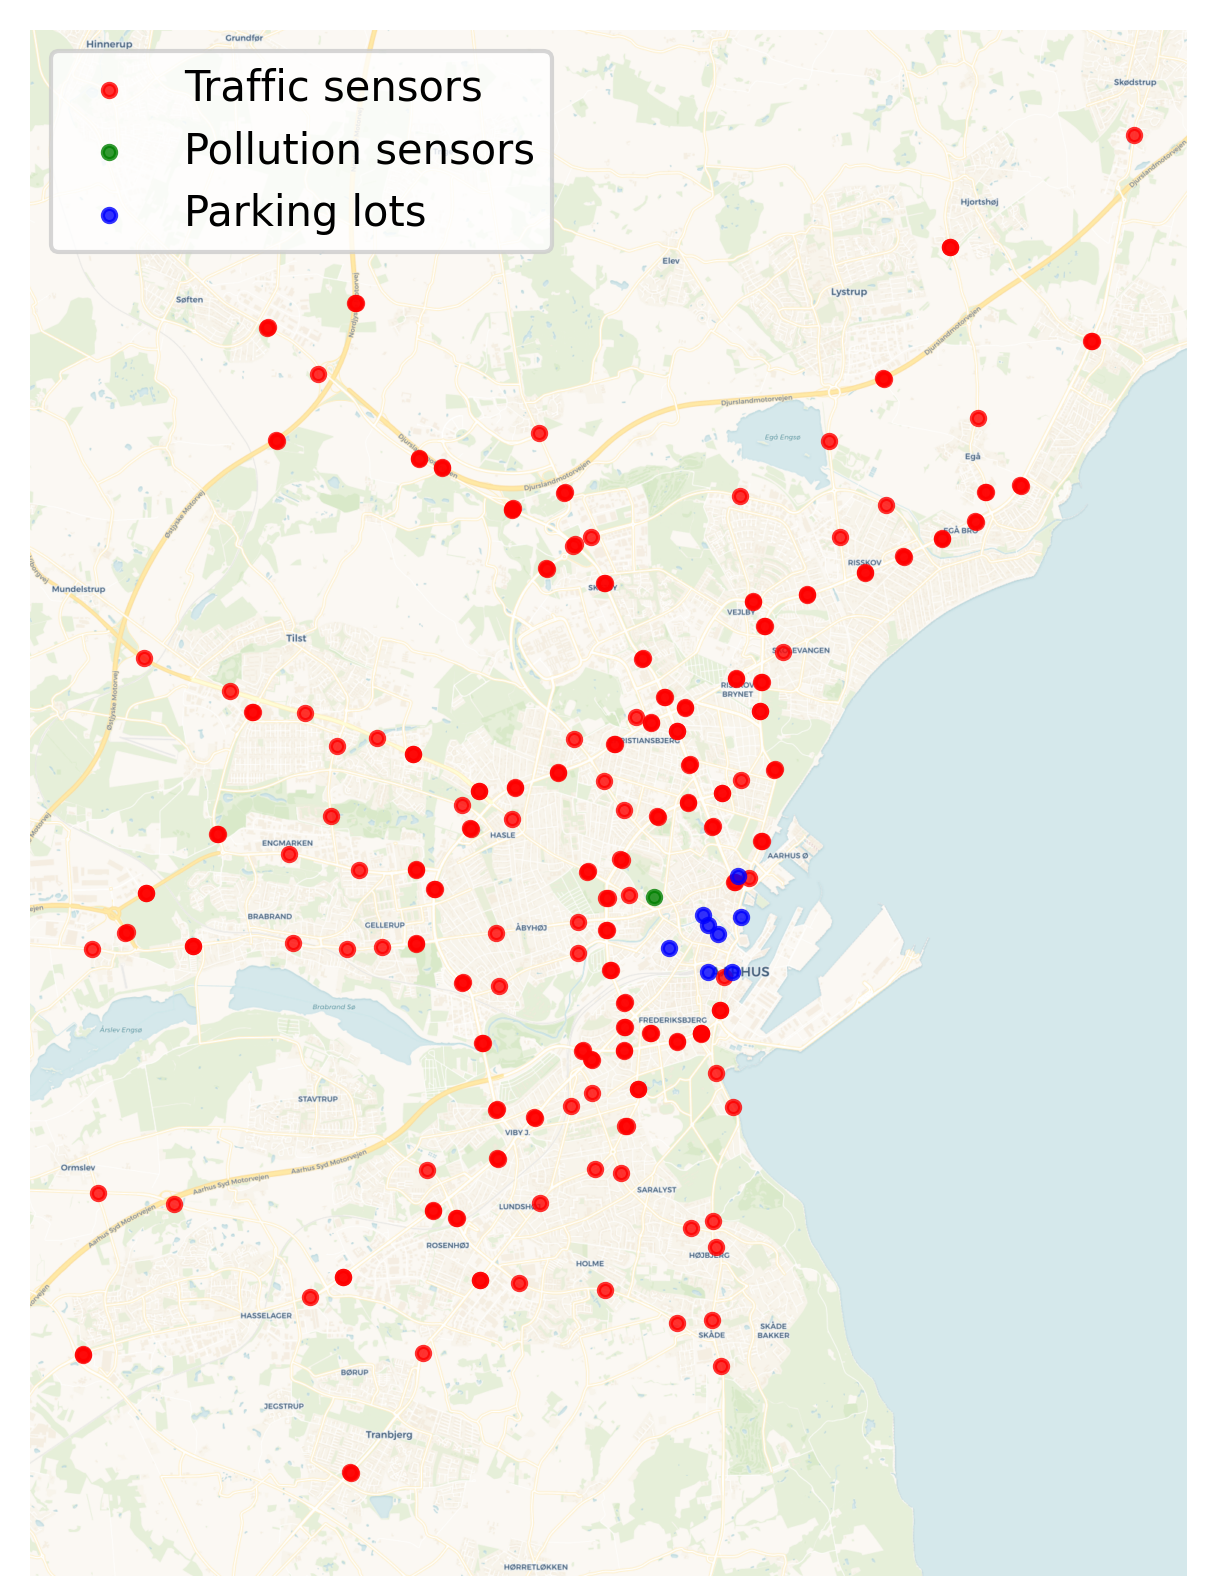
\includegraphics[width=0.5\linewidth]{images/aarhussensors.png}
    \caption{Map of Aarhus city sensors, in red are the traffic sensors, in green the only sensor for pollutants measurements, in blue the parking lots.}
    \label{fig:aarhus-sensors}
\end{figure}


\subsection{Seoul}
As mentioned in chapter \ref{subsec:ExamplesOfSmartCities}, the Seoul Metropolitan Government provides public air pollution data through the Open Data Plaza. However, the data for this activity is collected from Kaggle \cite{kaggleSeoul}, where the data for six pollutants (SO\textsubscript{2}, NO\textsubscript{2}, CO, O\textsubscript{3}, PM\textsubscript{10}, PM\textsubscript{2.5}) is already aggregated into a single table containing hourly observations from January 2017 to December 2019. 
In this dataset, observations from 25 stations located in different districts of Seoul are available. However, to make the results comparable between the three datasets, only one station is used for analysis and model training (Figure \ref{fig:SeoulSensors}).
To supplement the data with additional information, weather data were downloaded from the Open-Meteo website \cite{openMeteo}, which provides an API to download historical data with hourly granularity. 

\begin{table}[h]
\centering
\begin{tabular}{|c|c|}
\hline
\textbf{Category} & \textbf{Variables} \\ \hline
Air Pollution Observations & \begin{tabular}[c]{@{}c@{}}O\textsubscript{3}, PM\textsubscript{10}, PM\textsubscript{2.5},\\ NO\textsubscript{2}, CO, SO\textsubscript{2}\end{tabular} \\ \hline
Meteorological Data & \begin{tabular}[c]{@{}c@{}}temp, humidity, precip,\\ windspeed, cloudcover, rain, snow\end{tabular} \\ \hline
\end{tabular}
\caption{Variables in the Seoul Dataset. Description of each variable is found on Table \ref{apptable:Seoul_variable_description} in the appendix.}
\end{table}


\begin{figure}[h]
    \centering
    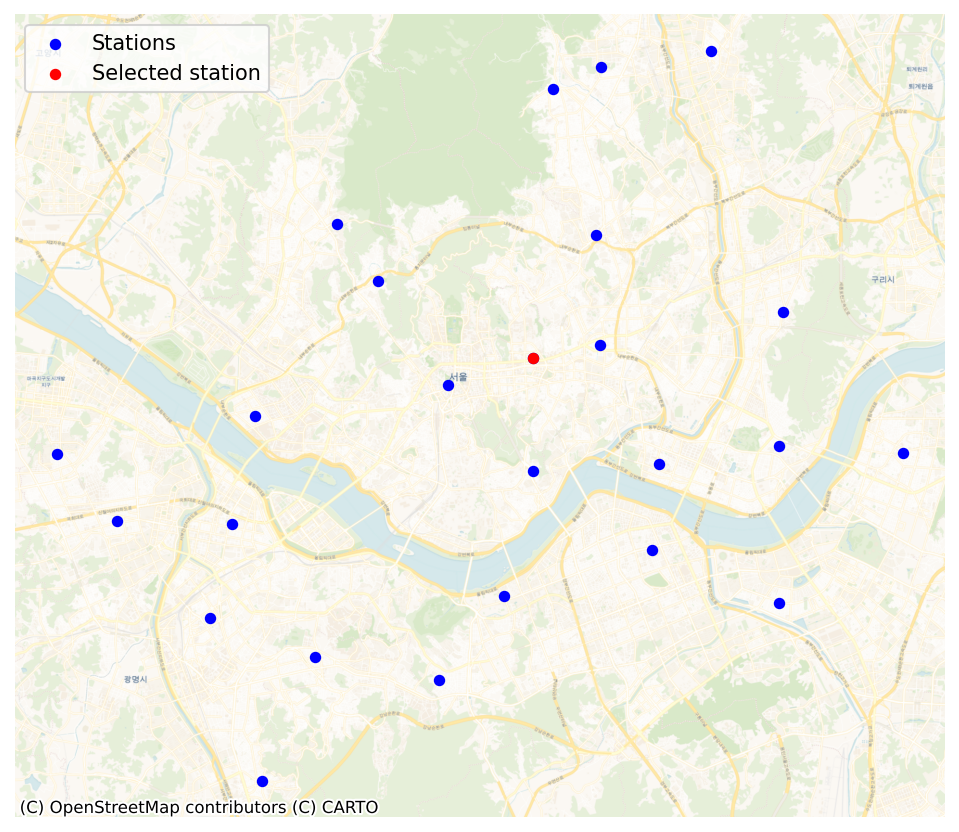
\includegraphics[width=0.5\linewidth]{images/seoulsensors.png}
    \caption{Seoul measurement stations across the districts. In red the station elected for this analysis.}
    \label{fig:SeoulSensors}
\end{figure}

\subsection{Madrid}
The air quality data for Madrid is publicly available on the Madrid's City Council Open Data website \cite{openDataMadrid}. Being data downloadable from the website in a confusing and not common format, and not well designed for general purpose use, a version of the dataset from Kaggle \cite{kaggleMadrid} has been used in this analysis.
In the DataFrame, particle measurements are recorded for each station, covering the period from January 2001 to April 2018, provided that the station was operational throughout this timeframe. It's important to note that stations differ in their equipment, leading to each station being capable of measuring only a specific subset of particles. For the purposes of this work, we have analyzed data from only one station (Figure \ref{fig:madridsensors}) that collects the six pollutants of interest, and the time range was restricted to three years (2015 - 2017). 
Missing data in some observations, were filled with the previous valid observation.
Again, weather data has been gathered from Open-Meteo website to add information to this dataset.

\begin{table}[h]
\centering
\begin{tabular}{|c|c|}
\hline
\textbf{Category} & \textbf{Variables} \\ \hline
Air Pollution Observations & \begin{tabular}[c]{@{}c@{}}PM\textsubscript{10}, PM\textsubscript{2.5}, NO\textsubscript{2}, \\ CO,	SO\textsubscript{2}, O\textsubscript{3}\end{tabular} \\ \hline
Meteorological Data & \begin{tabular}[c]{@{}c@{}}temp, humidity, dew, precip,\\ rain, snow, pressure, windspeed, \\ cloudcover, winddir\end{tabular} \\ \hline
\end{tabular}
\caption{Variables in the Madrid Dataset. Description of each variable is found on Table \ref{apptable:madrid_variable_description} in the appendix.}
\end{table}


\begin{figure}[h]
    \centering
    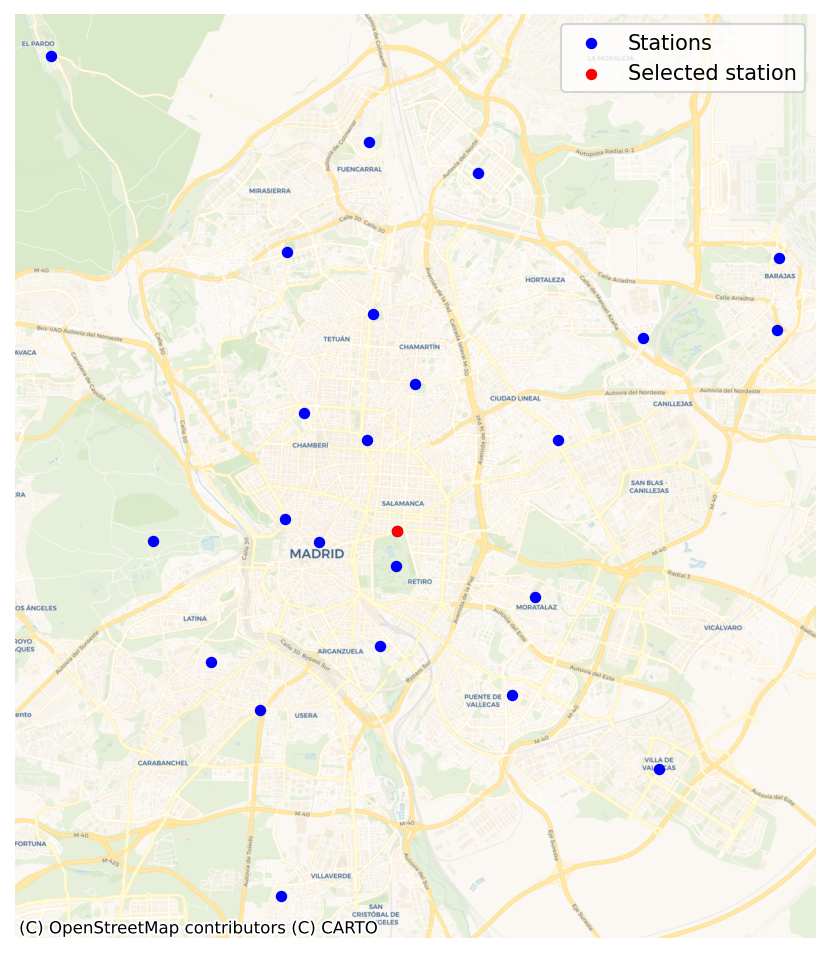
\includegraphics[width=0.5\linewidth]{images/madridsensors.png}
    \caption{Madrid measurement stations. In red the station elected for this analysis.}
    \label{fig:madridsensors}
\end{figure}

\newpage
\section{Explorative data analysis}
In this section is provided a brief data analysis to understand the dataset properties.

\subsection{Citypulse}

The graphical representation (Figure \ref{fig:ts_citypulse}) reveals that the time series of all four pollutants exhibit irregular and variable trends. The Ozone and PM\textsubscript{2.5} variables demonstrate nearly identical, on average decreasing patterns. Conversely, the PM\textsubscript{10} historical series displays a more sporadically linear trend, especially during descents, likely attributed to atmospheric events such as rainfall. The NO\textsubscript{2} historical series follows a less linear trend, frequently approaching zero. Notably, an anomalous trend occurs in the first week of October, which can be attributed to the interpolation method employed for handling missing data.

\begin{figure}[h]
    \centering
    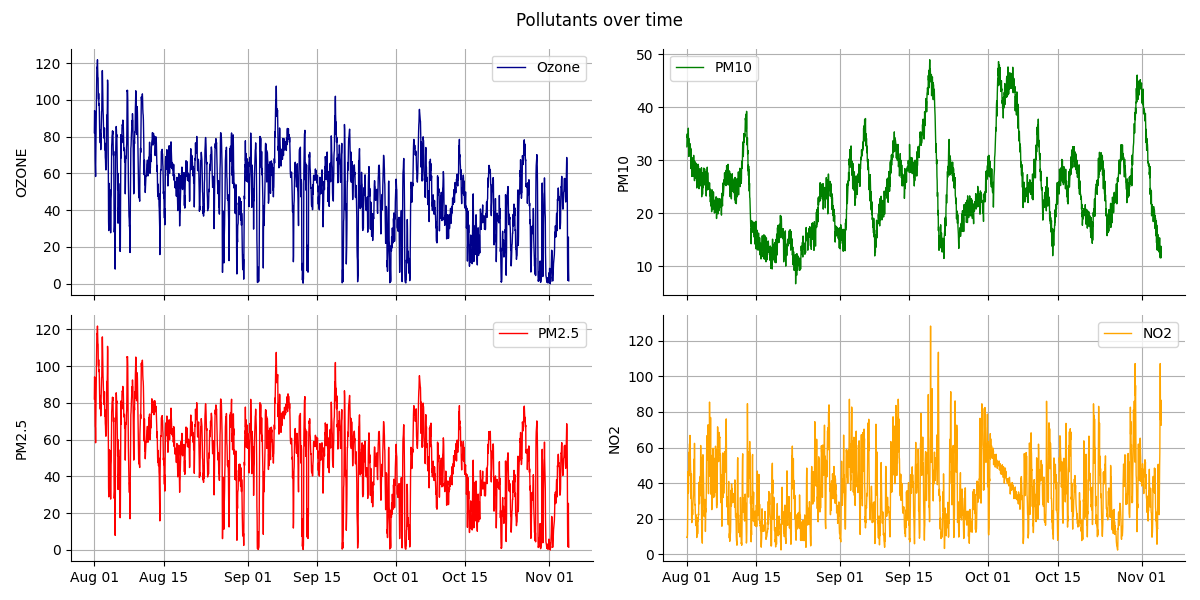
\includegraphics[width=1\linewidth]{images/ts_citypulse.png}
    \caption{Pollutant concentrations over time for the Citypulse dataset}
    \label{fig:ts_citypulse}
\end{figure}

Let us now examine the correlation among all variables in the dataset (Figure \ref{fig:corr_matrix_citypulse}):
\begin{itemize}[noitemsep]

    \item The variables "occupied" and "occupancy" are naturally correlated, as one is computed based on the other.
    \item "temp" and "feelslike" exhibit a strong positive correlation, nearly perfect at 0.995244, as expected since they represent similar measurements of meteorological conditions.
    \item The two target variables, ozone and PM\textsubscript{2.5}, are perfectly correlated, and this should be taken into consideration in model construction.
    \item Ozone and PM\textsubscript{2.5} variables show positive correlations with the "temp" and "feelslike" variables, suggesting a potential association between these variables.
    \item Unexpectedly, the PM\textsubscript{10} and PM\textsubscript{2.5} variables do not show a strong correlation, as would be expected and we will see instead in the other two datasets.
\end{itemize}

\begin{figure}[h]
    \centering
    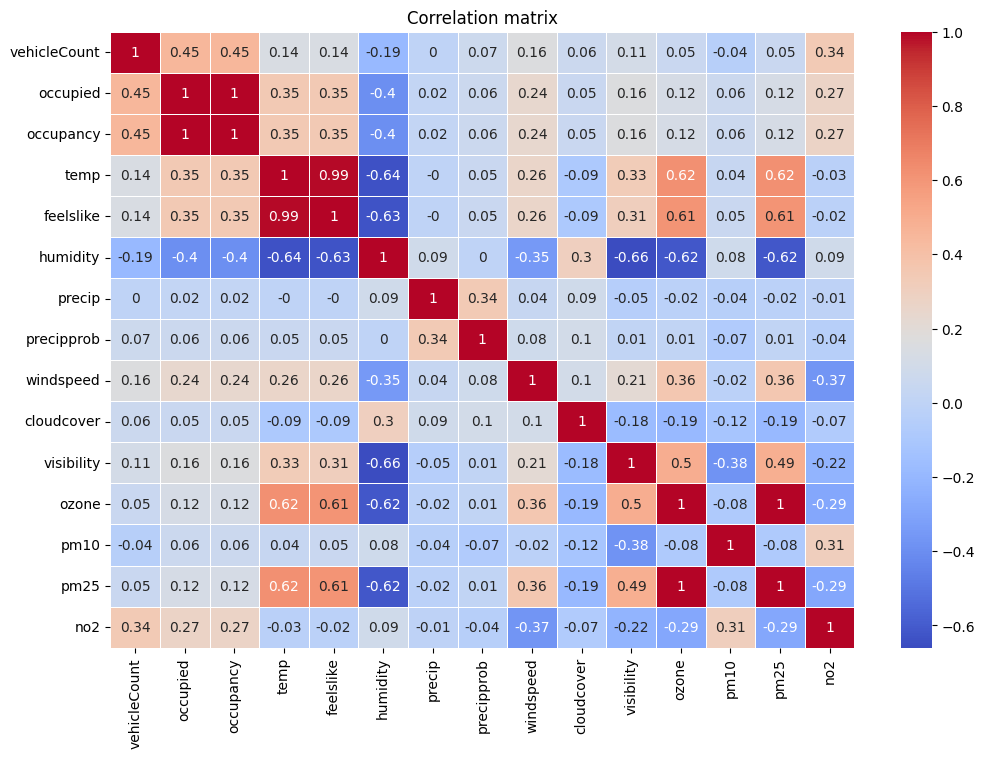
\includegraphics[width=0.75\linewidth]{images/corr_matrix_citypulse.png}
    \caption{Correlation matrix between the variables of the Citypulse dataset.}
    \label{fig:corr_matrix_citypulse}
\end{figure}

\newpage
\subsection{Seoul}

Analyzing the time series of pollutants in Seoul (Figure \ref{fig:ts_seoul}) reveals several distinct patterns. In the cases of SO\textsubscript{2} and CO, peaks coincide on specific dates. Notably, CO levels constitute approximately 10\% of SO\textsubscript{2} levels. However, peak durations are limited to 2-3 observations, followed by an abrupt decline, raising concerns about observation accuracy. 
A similar pattern emerges in PM\textsubscript{10} and PM\textsubscript{2.5}, underscoring the correlation between these two series. The historical O\textsubscript{3} series exhibits elevated levels during warmer months, contrasting with lower levels during colder months.
Conversely, NO\textsubscript{2} displays an opposing trend, with reduced variability in warmer months and elevated levels in colder months. 

\begin{figure}[h]
    \centering
    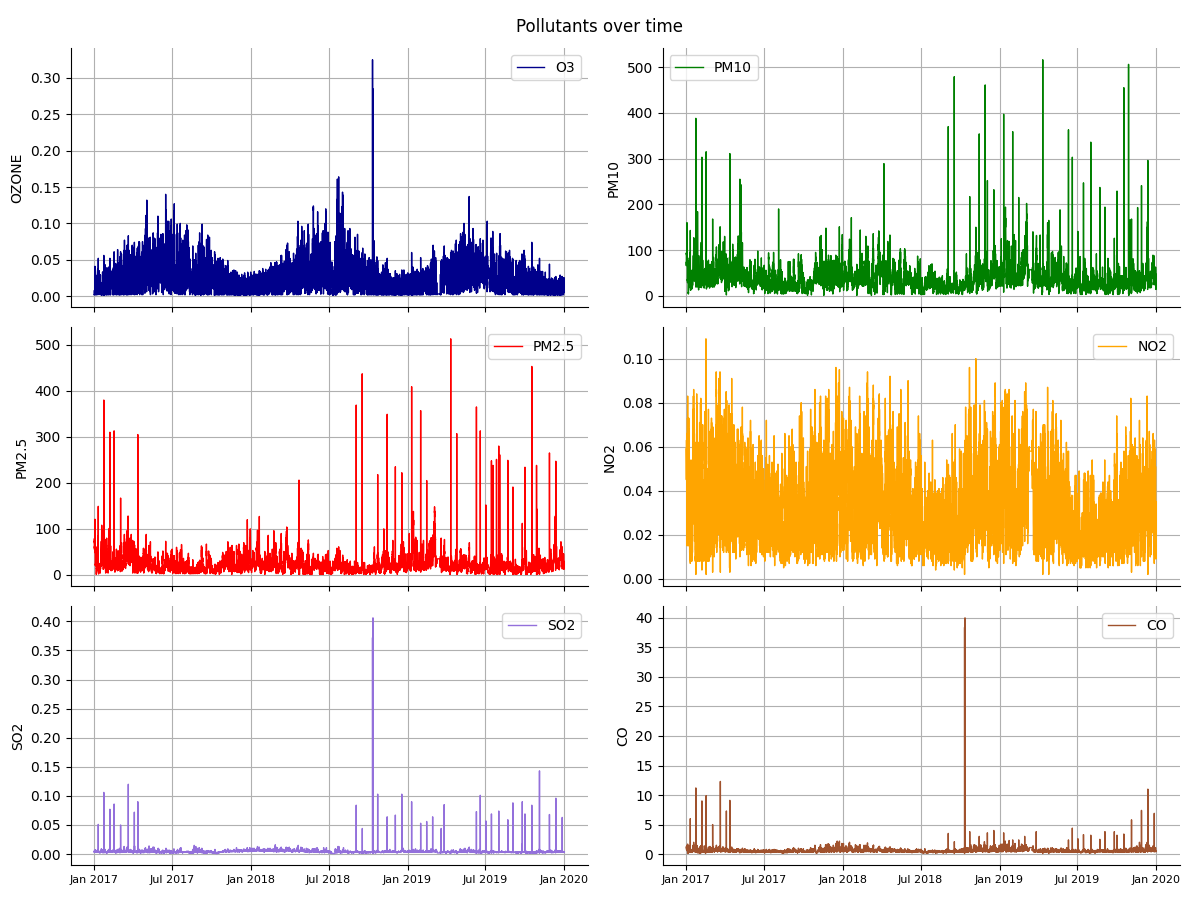
\includegraphics[width=1\linewidth]{images/ts_seoul.png}
    \caption{Pollutant concentrations over time for the Seoul dataset}
    \label{fig:ts_seoul}
\end{figure}


As observed in the plots, substantial correlations are evident in the correlation matrix (Figure \ref{fig:corr_matrix_seoul}):

\begin{itemize}[noitemsep]
    \item CO and SO\textsubscript{2} exhibit a strong positive correlation (0.79).
    \item PM\textsubscript{2.5} and PM\textsubscript{10} display a notable positive correlation (0.8).
    \item A significant positive correlation is noted between PM\textsubscript{2.5} and CO (0.65).
\end{itemize}
Further insights include a negative correlation between NO\textsubscript{2} and O\textsubscript{3} (-0.55), signifying an inverse relationship. Additionally, we can see the lack of correlation between wind speed and PM\textsubscript{2.5} (-0.031) and PM\textsubscript{10} (0.036) is affirmed, indicating no significant linear relationship, contrary to what might be expected.

\begin{figure}[h]
    \centering
    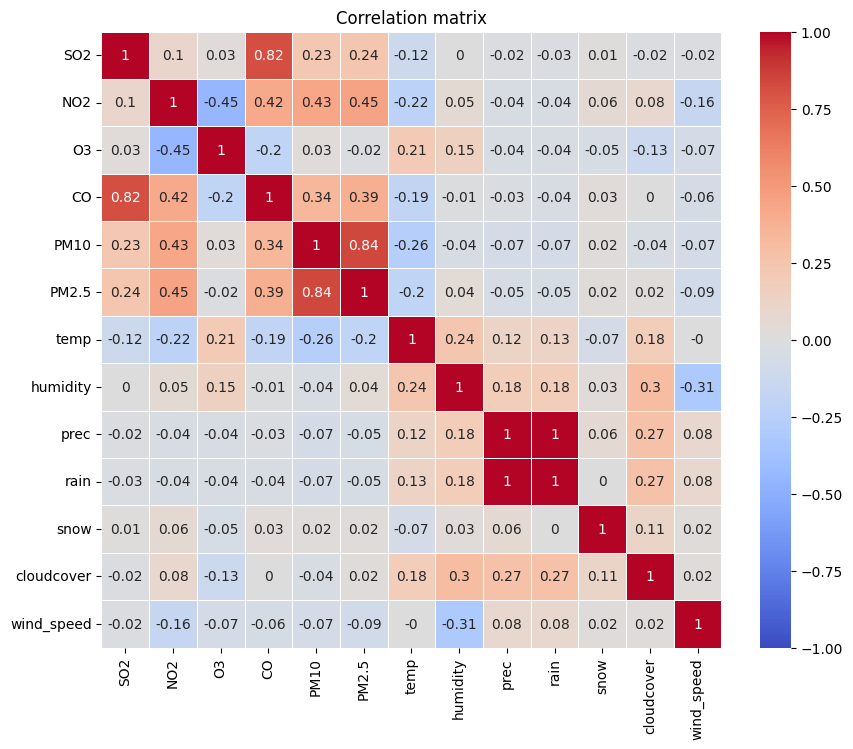
\includegraphics[width=0.75\linewidth]{images/corr_matrix_seoul.png}
    \caption{Correlation matrix between the variables of the Seoul dataset.}
    \label{fig:corr_matrix_seoul}
\end{figure}

\newpage
\subsection{Madrid}
Examining the plots (Figure \ref{fig:ts_madrid}) yields insightful observations:
the behavior of PM\textsubscript{10} and PM\textsubscript{2.5} demonstrates a striking similarity, implying a close connection between these particulate matter metrics.
SO\textsubscript{2} presents an anomalous linear growth in 2017 from April to November, followed by a subsequent return to lower levels. This peculiar pattern suggests a potential sensor replacement, likely occurring in both November 2017 and July 2016.
Nitric dioxide (NO) exhibits high variability, indicative of dynamic fluctuations, yet maintains an overall stable trend, highlighting consistent concentrations of this pollutant.
In alignment with the historical Seoul data, O\textsubscript{3} concentrations follow a seasonal dynamic, increasing during warmer months and decreasing in winter. This cyclical pattern reflects the climatic influence on ozone levels.

\begin{figure}[h]
    \centering
    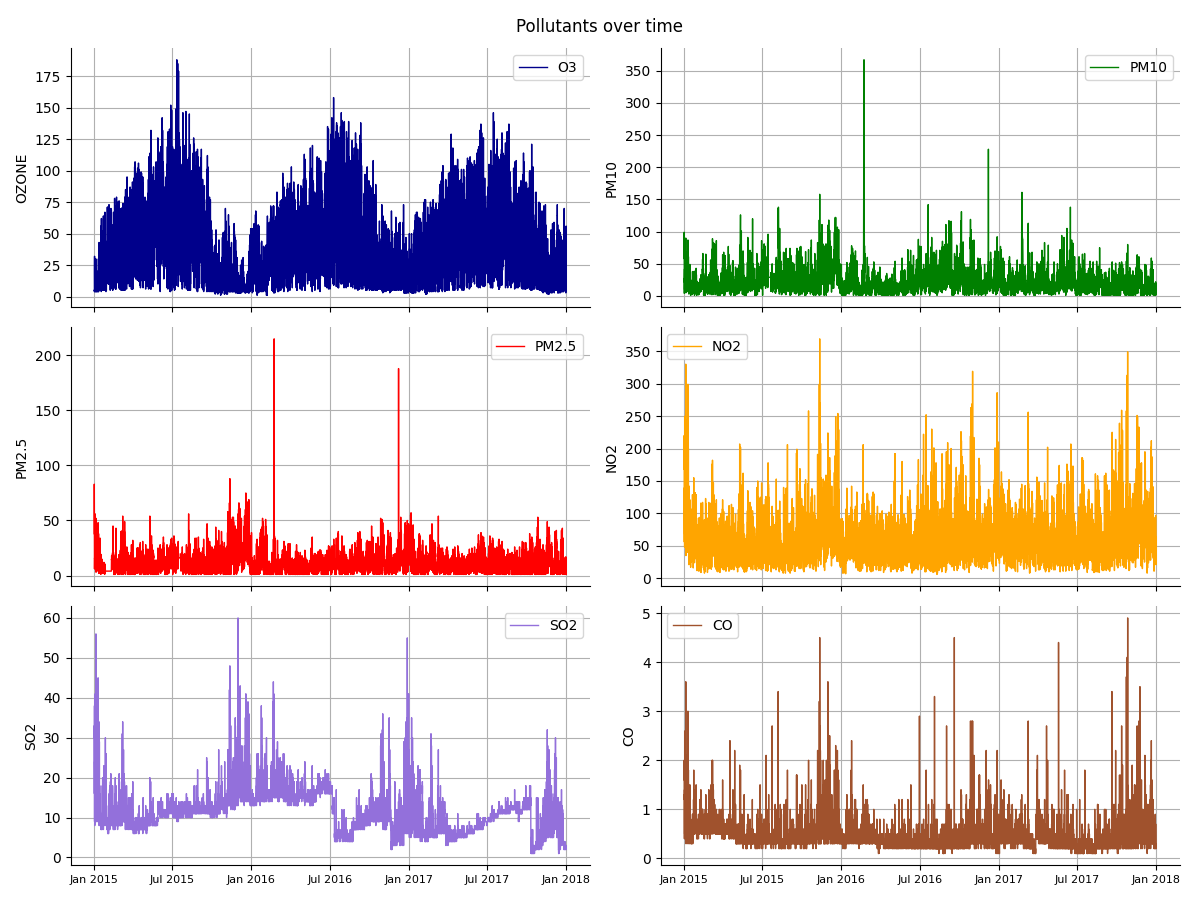
\includegraphics[width=1\linewidth]{images/ts_madrid.png}
    \caption{Pollutant concentrations over time for the Madrid dataset}
    \label{fig:ts_madrid}
\end{figure}

The correlation matrix (Figure \ref{fig:corr_matrix_madrid}) analysis reveals noteworthy connections: 
\begin{itemize}
    \item  A strong positive correlation (0.72) indicates a significant association between carbon monoxide (CO) and nitrogen dioxide (NO\textsubscript{2}), suggesting shared emission sources or interdependence in atmospheric processes.
    \item A high positive correlation (0.85) between PM\textsubscript{2.5} and PM\textsubscript{10} again suggests a robust coherence in the dynamics of fine and coarse particulate matter, indicative of shared sources or mutual influences.
    \item A notable negative correlation (-0.56) between nitrogen dioxide (NO\textsubscript{2}) and ozone (O\textsubscript{3}) suggests an antagonistic interaction, potentially influenced by disparate sources or chemical reactions in the atmosphere. This pattern is consistent with findings in the Seoul dataset.
\end{itemize}

\begin{figure}[h]
    \centering
    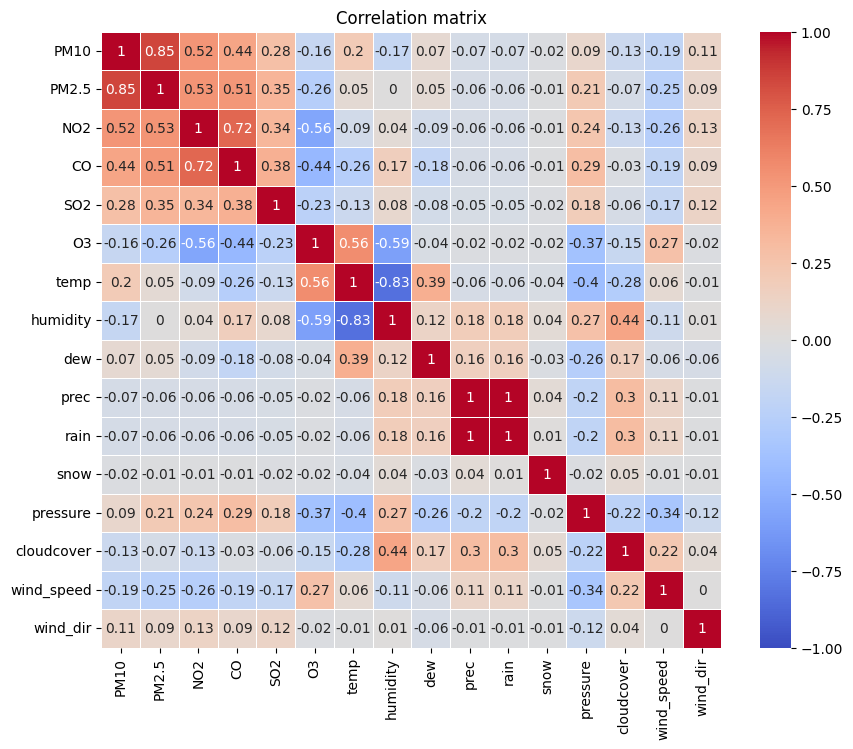
\includegraphics[width=0.75\linewidth]{images/corr_matrix_madrid.png}
    \caption{Correlation matrix between the variables of the Madrid dataset.}
    \label{fig:corr_matrix_madrid}
\end{figure}

\newpage
\section{In-depth analysis}

The subsequent phase of the dataset analysis will be dedicated exclusively to time series analysis. However, before delving into this analysis, it is useful to introduce three fundamental concepts that will enhance comprehension of the forthcoming examination.

\paragraph{Seasonal decomposition:}Seasonal decomposition is a statistical technique employed to dissect time series data into fundamental components, namely trend, seasonality, and residual. The trend signifies long-term alterations, elucidating the overall trajectory of the data; seasonality captures cyclic patterns within predefined time intervals; and residual accounts for the stochastic variation that remains subsequent to the consideration of both trend and seasonality.
This method serves diverse purposes, such as \textbf{pattern identification}, removal of seasonal effects, enhancement of predictive capabilities, and facilitation of \textbf{comparative analysis}. Notably, the technique can manifest as either additive, wherein components are amalgamated through addition, or multiplicative, where the components are combined through multiplication. The selection of the appropriate method hinges upon the nature of the time series under examination.

\paragraph{Autocorrelation Function (ACF) and Autocorrelation Plot:}The Autocorrelation Function (ACF) is a statistical measure assessing the correlation between a given data point and its preceding points within the same time series. It aids in identifying trends or relevant periodic patterns in past observations. In an ACF plot, values above the dashed line signify positive correlations, while those below indicate negative correlations. Significant peaks outside the confidence interval denote time lags with strong correlations, suggesting potential patterns or seasonality in the time series.

\paragraph{Partial Autocorrelation Function (PACF) and Partial Autocorrelation Plot:}The Partial Autocorrelation Function (PACF) is a measure evaluating the correlation between a given data point and its previous points, accounting for the influence of intervening lags. It proves useful in identifying the direct correlation between a data point and past points without the influence of intermediate lags. In the PACF plot, peaks outside the confidence interval represent time lags with significant correlations not explained by intervening lags. These peaks assist in directly pinpointing relationships between data points, highlighting the most immediate and relevant correlations in the time series. However, interpreting the PACF plot can be difficult by definition.

% TODO - Qua non saprei se includere i plot della PACF oppure no, perchè comunque non ne estraiamo informazioni, sarebbe più un discorso di completezza che di utilità
Usually, ACF and PACF plots are useful to determine the best parameters for the definition of an ARIMA model. However, this is not the case, as these are used only to understand what is the relationship between observations at different times, and the focus will be only on the ACF plot, as it's interpretation in more intuitive and useful for this analysis.

\subsection{Citypulse}
Decomposition of the Aarhus pollutants time series has been carried out using an additive method, setting a period of 168 (24 observations per day * 7 days per week) to accentuate weekly seasonality. Figure \ref{fig:seasonality_aarhus} showcases the results, providing valuable insights into the observed patterns:

\begin{figure}[h]
    \centering
    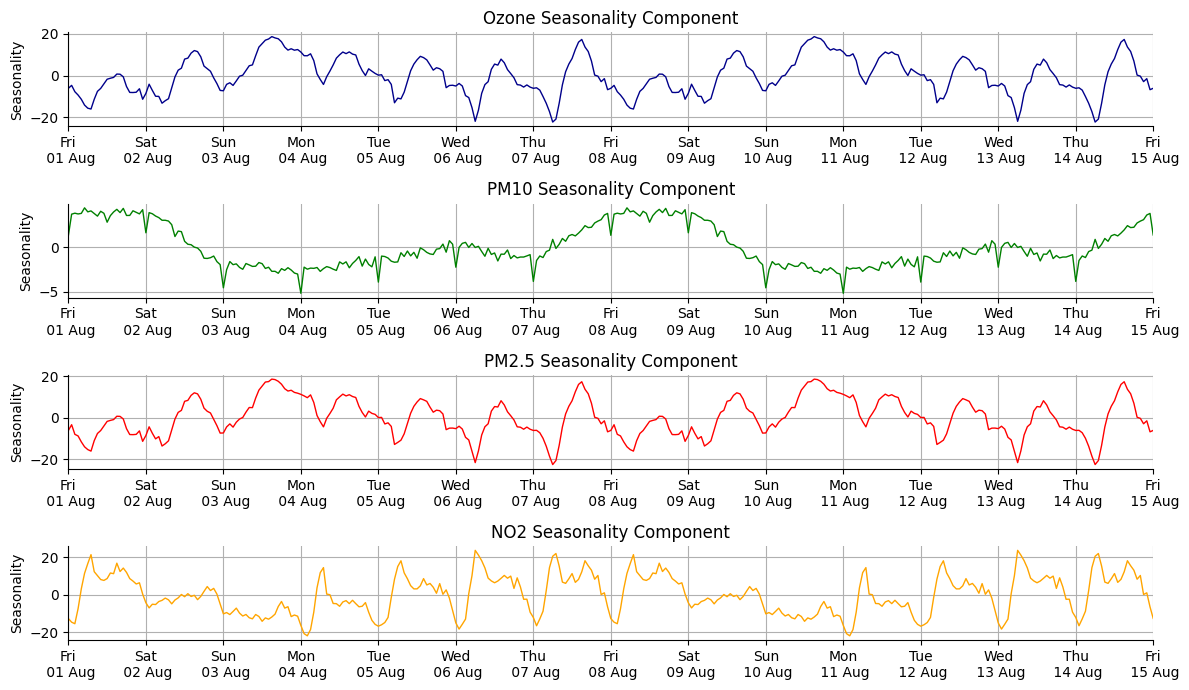
\includegraphics[width=1\linewidth]{images/citypulse_seasonality.png}
    \caption{Seasonal components of Aarhus's pollutants, focusing on a two-week period.}
    \label{fig:seasonality_aarhus}
\end{figure}

\begin{itemize}[noitemsep]
\item The seasonal components of Ozone and PM\textsubscript{2.5} exhibit identical patterns. These patterns manifest in two discernible trends: firstly, a reduction in pollutant levels during nighttime hours, followed by an increase during daytime. Secondly, during weekends, the average values of the series demonstrate a tendency to be lower.
\item The seasonal component of PM\textsubscript{10} displays a comparable pattern, wherein it experiences a decline from Saturday to Monday, followed by an increase during weekdays, reaching its zenith on Fridays and Saturdays. However, a unique behavior is observed in PM\textsubscript{10} that is absent in other series, characterized by a precipitous decline in observations at midnight, succeeded by a marked increase in subsequent observations.
\item NO\textsubscript{2} demonstrates a behavior akin to that of Ozone and PM\textsubscript{2.5}, with higher values observed during weekdays and lower values from Saturday to Monday.
\end{itemize}

Moving forward, present plots illustrating the autocorrelation function are presented. With respect to the ACF and a scrutiny of the plots (depicted in Figure \ref{fig:acfplot_citypulse}), several considerations can be derived:

\begin{figure}[h]
    \centering
    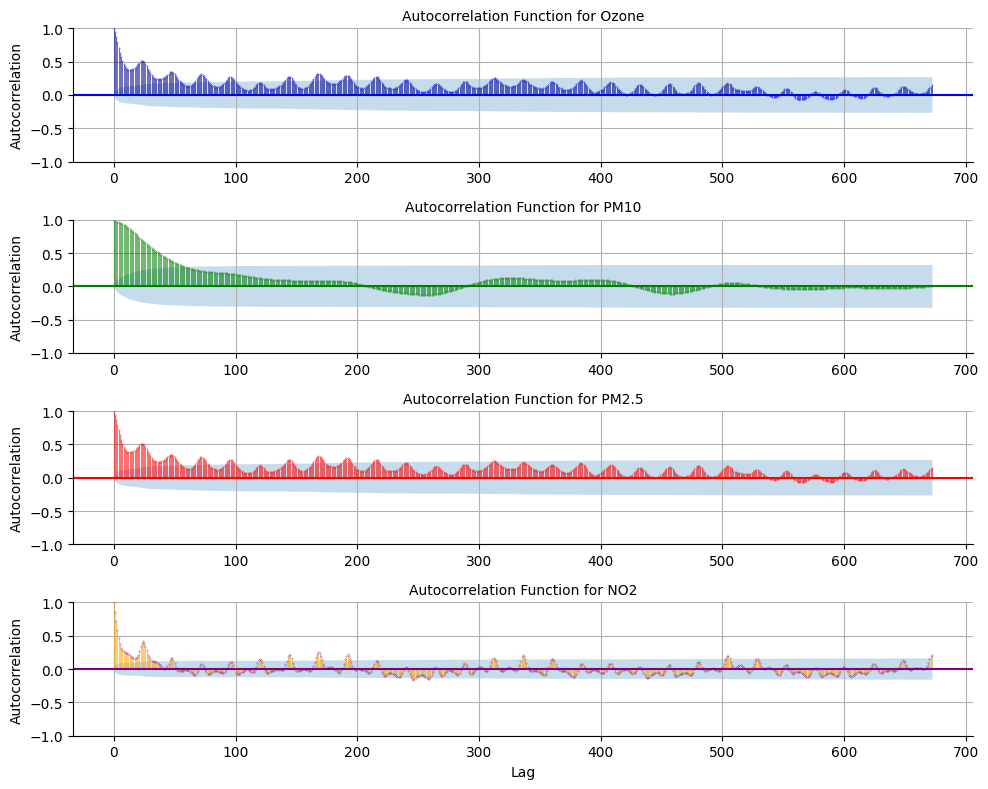
\includegraphics[width=1\linewidth]{images/acfplot_citypulse.png}
    \caption{ACF Plot for pollutants in Aarhus, displaying the first 700 values of the autocorrelation function.}
    \label{fig:acfplot_citypulse}
\end{figure}

\begin{itemize}[noitemsep]
    \item \textbf{O\textsubscript{3}:}
    The autocorrelation function computed on the ozone time series (similar to that of PM\textsubscript{2.5}) reveals spikes every 24 lags, indicating a daily seasonality. Additionally, a subtle increase is observed every 168 lags, suggesting a weekly seasonality.
    \item \textbf{PM\textsubscript{10}:}
    Contrary to ozone and PM\textsubscript{2.5}, the autocorrelation function for the PM\textsubscript{10} time series does not exhibit distinct patterns. Observations seem to be simply correlated with the approximately preceding 50 observations.
    \item \textbf{NO\textsubscript{2}:}
    Autocorrelation analysis of the NO\textsubscript{2} time series demonstrates a pronounced spike every 24 lags, corresponding to a daily seasonality. Furthermore, there is a growth trend every 168 lags, indicating a weekly seasonality. This suggests that observations are correlated not only within a day or two but also over the span of one or two weeks.

\end{itemize}






\subsection{Seoul}
Seoul pollutants time series have been decomposed using additive method, specifying a period of 168 (24 observations per day * 7 days per week), in order to highlight seasonality between weeks.
From this analysis (Figure \ref{fig:seasonality_seoul}) we can note several things:

\begin{figure}[h]
    \centering
    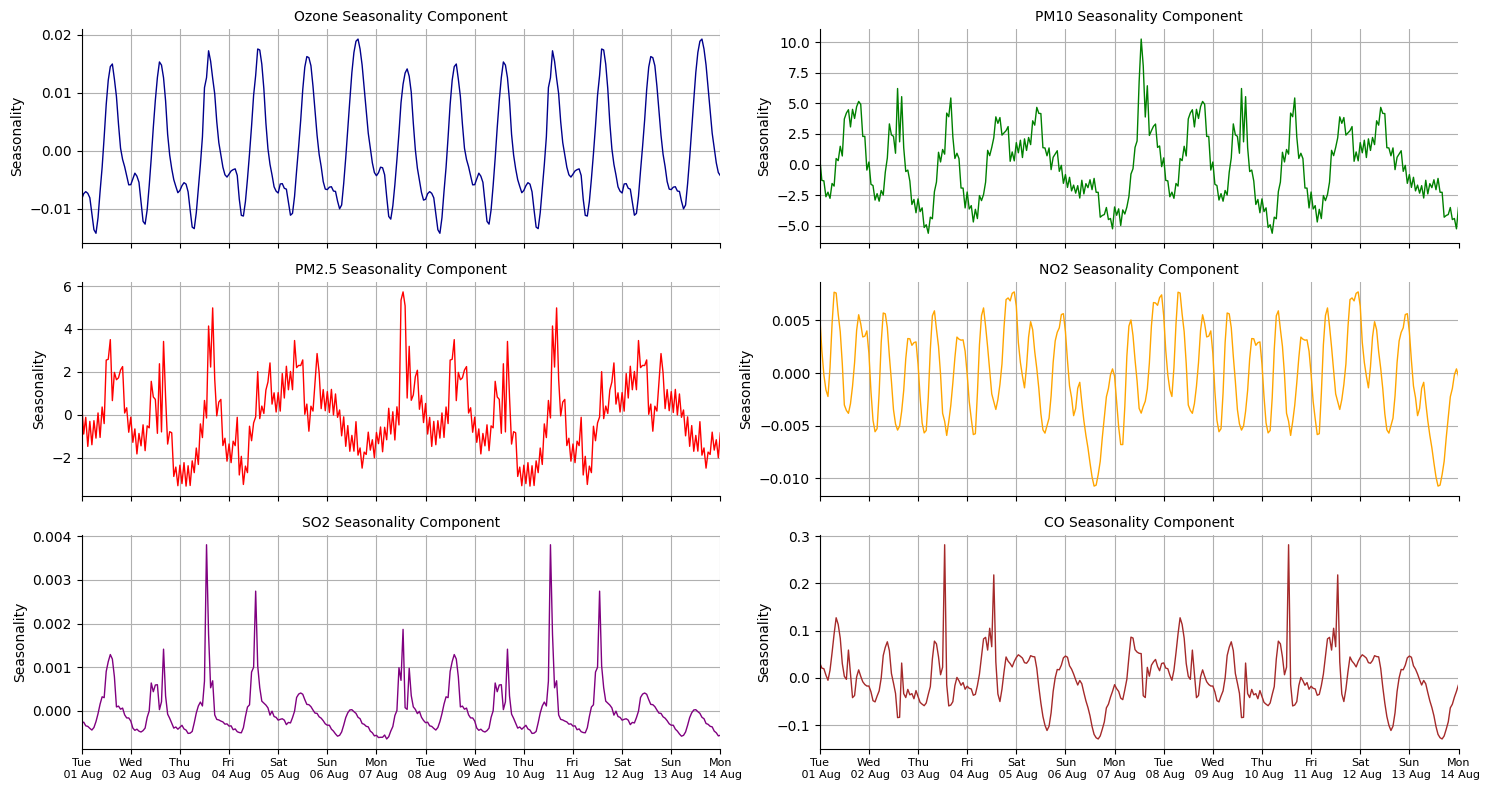
\includegraphics[width=1\linewidth]{images/seoul_seasonality.png}
    \caption{Seasonal components of Seoul's pollutants, focusing on a two-week period.}
    \label{fig:seasonality_seoul}
\end{figure}

\begin{itemize}[noitemsep]
    \item \textbf{O\textsubscript{3}} shows peaks during the day, approximately around noon, and rapidly decreases towards the evening, reaching the minimum. Lower values are observed on Saturdays, Mondays, and Tuesdays.
    \item \textbf{PM\textsubscript{10}} decreases on Saturday, Sunday, and Monday, then increases during the week.
    \item \textbf{PM\textsubscript{2.5}}, in contrast to PM\textsubscript{10}, does not exhibit specific patterns, other than the usual increase during the day and decrease during the night.
    \item \textbf{NO\textsubscript{2}} shows two peaks per day, with the most significant peaks occurring on Saturdays, and negative peaks on Sundays.
    \item \textbf{SO\textsubscript{2}} exhibits peaks on weekdays and remains low during the weekend.
    \item \textbf{CO} demonstrates a general increase throughout the week and a decrease over the weekend until Monday, where the lowest values are recorded.
\end{itemize}

Next, plots for the autocorrelation function are displayed. As for the ACF, looking at the plots (Figure \ref{fig:acfplot_seoul}), the following considerations can be made:

\begin{figure}[h]
    \centering
    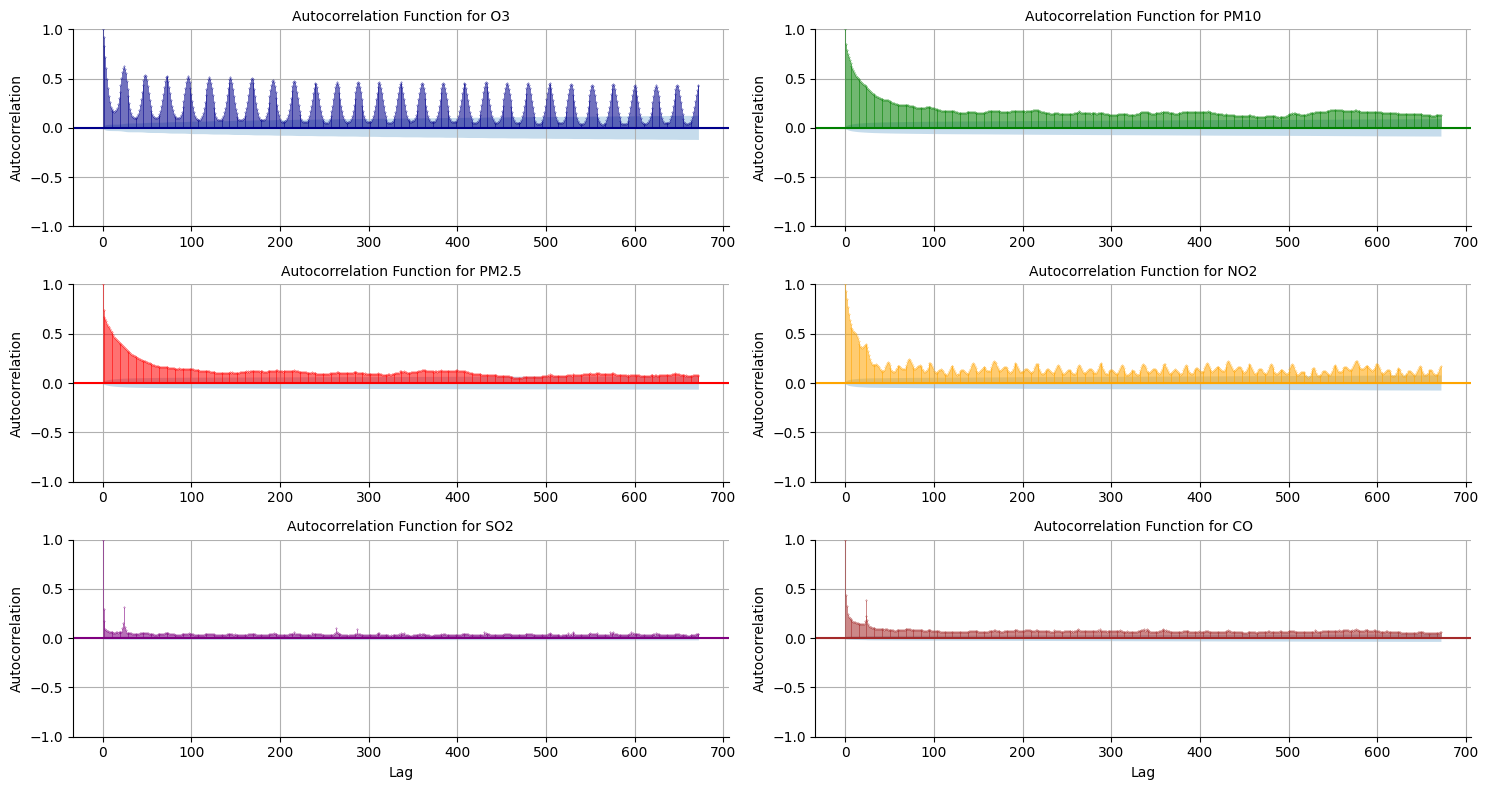
\includegraphics[width=1\linewidth]{images/acfplot_seoul.png}
    \caption{ACF Plot for pollutants in Seoul, displaying the first 700 values of the autocorrelation function.}
    \label{fig:acfplot_seoul}
\end{figure}

\begin{itemize}[noitemsep]
    \item \textbf{O\textsubscript{3}} exhibits clear daily seasonality, and there is also a subtle weekly seasonality discernible in the data.
    \item \textbf{PM\textsubscript{10} and PM\textsubscript{2.5}} demonstrate a robust autocorrelation in the initial approximately 60 observations, with a noticeable tendency towards weekly seasonality. However, daily seasonality is not prominently evident.
    \item \textbf{NO\textsubscript{2}} shows peaks approximately every 10 days, along with a strong autocorrelation in the first 24 observations.
    \item \textbf{SO\textsubscript{2}} exhibits daily peaks and some isolated, peculiar spikes that are challenging to explain.
    \item \textbf{CO:} does not display distinct peaks but shows a strong autocorrelation in the initial 24 observations.
\end{itemize}

\subsection{Madrid}
The time series of pollutants in Madrid underwent additive decomposition with a specified period of 168 (24 observations per day multiplied by 7 days per week). Seasonal components resulting from this process are displayed in Figure \ref{fig:madrid_seasonality}:

\begin{figure}[h]
    \centering
    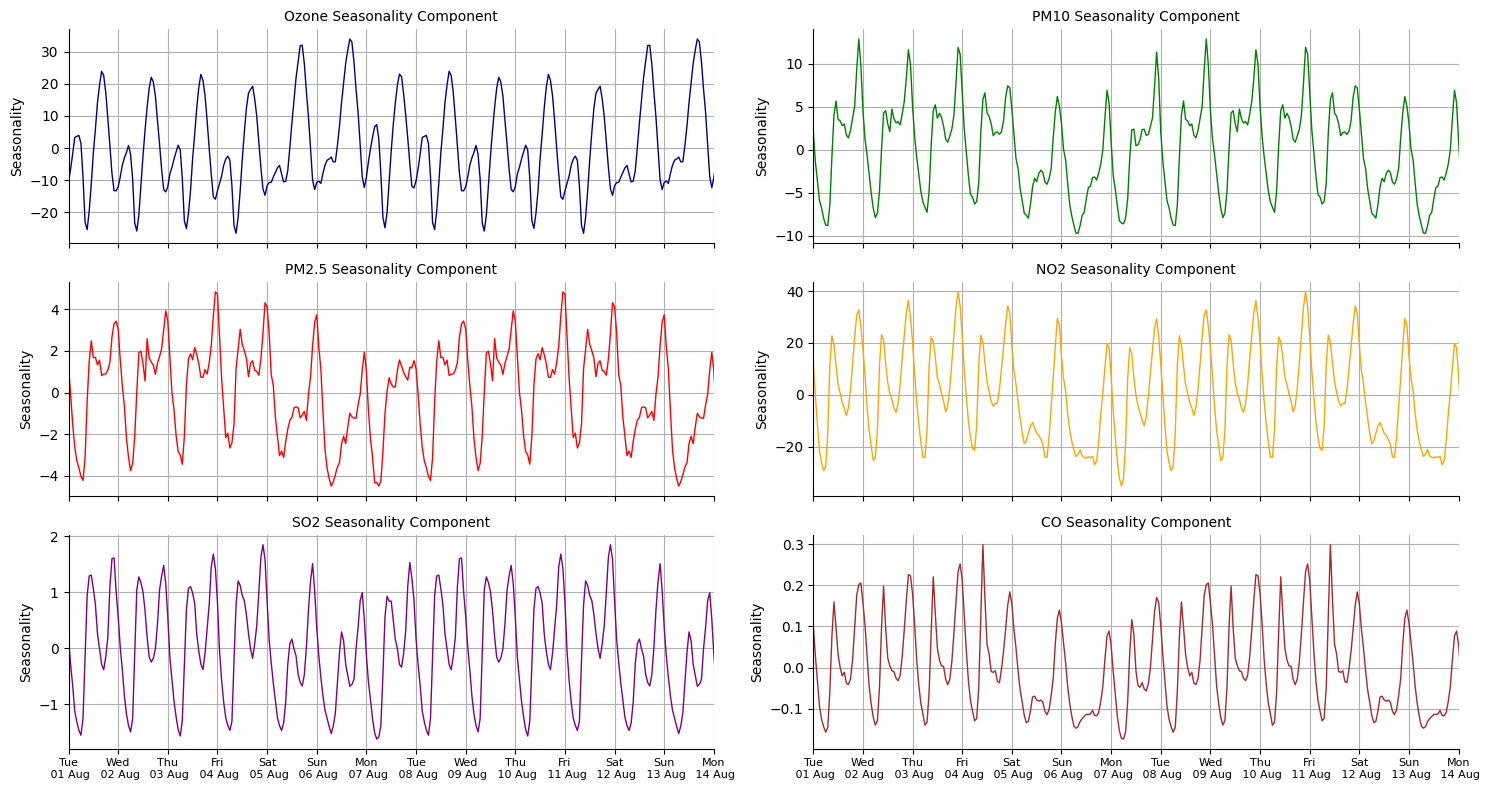
\includegraphics[width=1\linewidth]{images/madrid_seasonality.png}
    \caption{Seasonal components of Seoul's pollutants, focusing on a two-week period.}
    \label{fig:madrid_seasonality}
\end{figure}

\begin{itemize}[noitemsep]
    \item \textbf{O\textsubscript{3}} peaks during the day (around noon) and rapidly decreases towards the evening, reaching the minimum. Unlike other pollutants, the highest peaks are observed on weekends.
    \item \textbf{PM\textsubscript{10}} decreases on Friday, Saturday, and Sunday, and increases during the week.
    \item \textbf{PM\textsubscript{2.5}}, in contrast to the historical series in Seoul, follows the same pattern as PM\textsubscript{10}.
    \item \textbf{NO\textsubscript{2}} displays two peaks per day, with the most significant peaks occurring on Saturdays, and negative peaks on Sundays.
    \item \textbf{SO\textsubscript{2}} exhibits a seasonal component with higher variance on weekdays and lower variance on weekends.
    \item \textbf{CO} demonstrates a general increase throughout the week and a decrease over the weekend until Monday, where the lowest values are recorded.
\end{itemize}

Following this, the autocorrelation function plots are presented. Analyzing the ACF plots (Figure \ref{fig:acfplot_madrid}), the subsequent observations can be noted:

\begin{figure}[h]
    \centering
    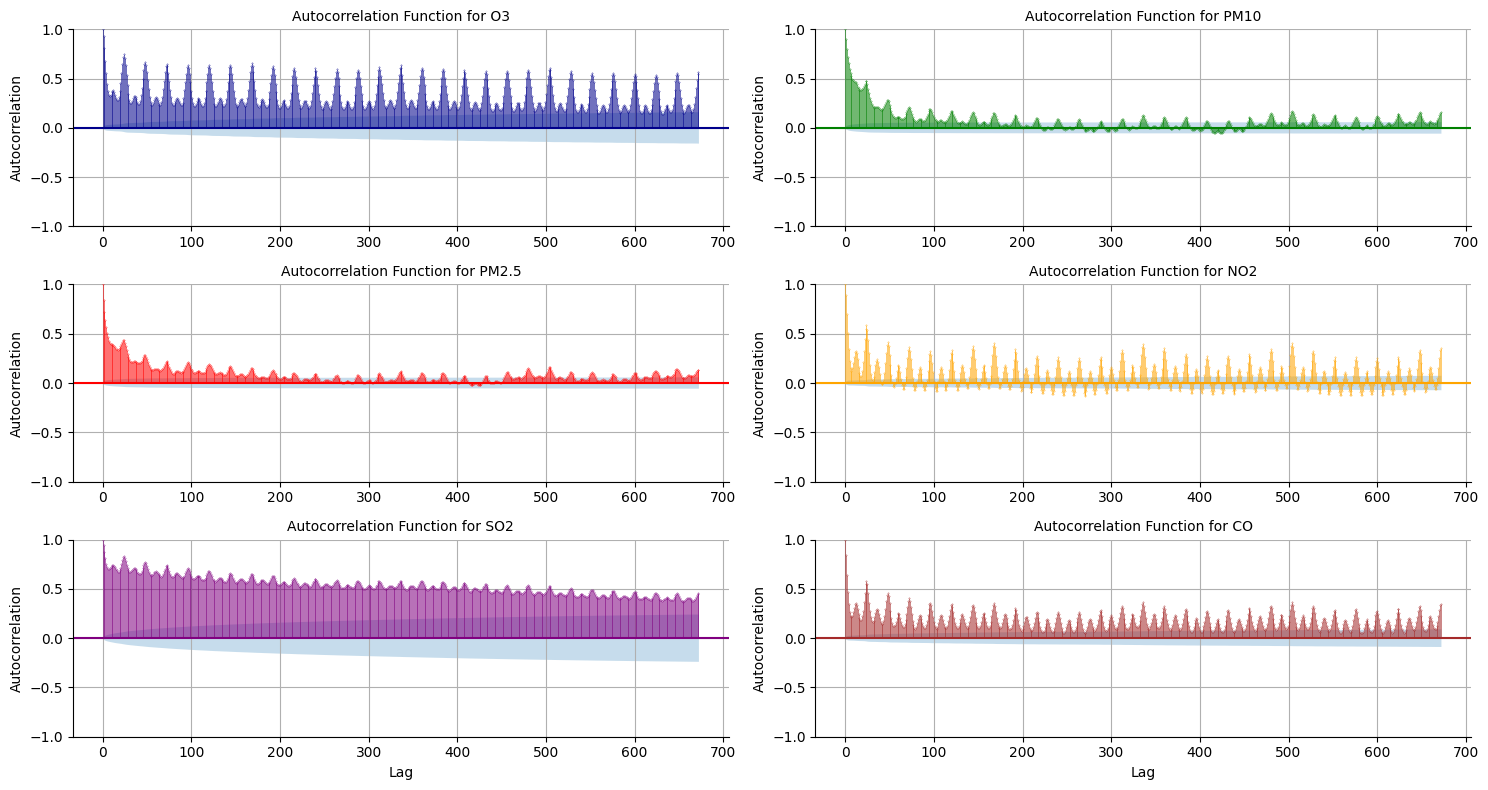
\includegraphics[width=1\linewidth]{images/acfplot_madrid.png}
    \caption{ACF Plot for pollutants in Madrid, displaying the first 700 values of the autocorrelation function.}
    \label{fig:acfplot_madrid}
\end{figure}

\begin{itemize}[noitemsep]
    \item \textbf{Ozone (O\textsubscript{3})} exhibits a conspicuous daily and intra-daily seasonality. Additionally, a subtle weekly seasonality is observable.
    \item \textbf{Particulate Matter (PM\textsubscript{10} and PM\textsubscript{2.5})} demonstrates a robust autocorrelation in the initial approximately 60 observations. Notably, there is an inclination towards bi-weekly seasonality, coupled with a distinct daily seasonality.
    \item \textbf{Nitrogen Dioxide (NO\textsubscript{2})} shows approximately every 7 days, together with a strong daily and intra-daily autocorrelation.
    \item \textbf{Sulfur Dioxide (SO\textsubscript{2})} features daily peaks and a pronounced initial autocorrelation that diminishes after numerous observations, likely influenced by the peculiar curve pattern.
    \item \textbf{Carbon Monoxide (CO)} displays a daily and intra-daily autocorrelation, alongside a subtle tendency towards weekly seasonality.
\end{itemize}

\newpage
\section{Conclusions}
In this chapter, an examination of the primary facets of the three datasets has been conducted, with a particular emphasis on the time series of pollutants. In order to consolidate the most significant characteristics of the datasets, the following summary table is presented.


\begin{table}[!ht]
    \centering
    
    \begin{tabular}{|l|l|c@{\hspace{4pt}}c@{\hspace{4pt}}c@{\hspace{4pt}}c@{\hspace{4pt}}c@{\hspace{4pt}}c|ccc|}
    \hline
        \multirow{2}{*}{Dataset} & \multirow{2}{*}{Duration} & \multicolumn{6}{c|}{Available pollutants} & \multicolumn{3}{c|}{External features} \\ \cline{3-11}
        & & O3 & PM10 & PM2.5 & NO2 & SO2 & CO & Traffic & Parkings & Weather \\ \hline
        Citypulse & 3 Months & \checkmark & \checkmark & \checkmark & \checkmark & ~ & ~ & 1 & 1 & 7 \\ \hline
        Seoul & 3 Years & \checkmark & \checkmark & \checkmark & \checkmark & \checkmark & \checkmark & 0 & 0 & 7 \\ \hline
        Madrid & 3 Years & \checkmark & \checkmark & \checkmark & \checkmark & \checkmark & \checkmark & 0 & 0 & 10 \\ \hline
    \end{tabular}
    \caption{Summary table of the Datasets}
    
\end{table}


The intricacies revealed through these analyses, despite their inherent complexity, prove to be invaluable for comprehending the inherent properties of the respective time series. The identification of distinctive patterns provides essential insights into the temporal dynamics of the environmental variables under consideration.

These findings constitute a crucial foundation for the subsequent stages of model development, where informed decisions must be made regarding the selection of appropriate architectures and parameter configurations. By leveraging the discerned temporal patterns, we can strategically tailor the model definition and data preparation steps to capture and exploit the underlying structures within the time series data.


\chapter{Developed Models}
\label{chap:Models}

This chapter aims to explore two key elements in time series analysis: data preparation and model architectures. Effective manipulation and organization of information is a key prerequisite to facilitate learning from a forecasting model due to the high complexity of temporal data. The first section of this chapter will focus on the methodology and techniques used to prepare temporal data, outlining selected practical approaches to address specific challenges noted in the chosen data.

The following section will shift the focus to model architectures. Several architectural paradigms will be examined, with particular emphasis on advanced solutions that have demonstrated significant impact in the time series prediction task, some already anticipated in Section \ref{cap1:sota}.

\section{Data Preparation}
\label{sec:DataPreparation}

The principal function of data preparation is to locate relevant characteristics in datasets and then modify the data in order to maximize model performance. This crucial procedure comes before model training, greatly enhancing the prediction power of the models.

To extract pertinent information from raw data, which is frequently heterogeneous and unstructured, considerable selection is required. Data cleansing, controlling outliers, addressing missing values, and guaranteeing data consistency are all part of the first step of data preparation. By interacting, these measurements help to create a more refined dataset, which serves as the foundation for further analytical procedures.

\subsection{Feature engineering and selection}
Feature selection and design in a machine learning model involves choosing the most important features for the model and creating ad hoc features to aid learning. 
\textbf{Feature selection} is the process of selecting a subset of relevant features for use in building the model.
Feature selection techniques are used for several reasons, including simplifying models to make them more easily interpretable, reducing training times, and avoiding the curse of dimensionality.
In our case, feature selection is utilized to eliminate redundant exogenous variables based on their correlation.
For example, in CityPulse, feelslike and occupied variables are removed, while temp and occupancy are kept. In Seoul and Madrid, rain is kept and prec is removed
On the other hand, \textbf{feature engineering} involves extracting features from raw data to support training.
In this case, feature engineering is used to extract \textbf{date-based features} such as the day of the week, month of the year, and time of day, which can be valuable for forecasting. As we have observed, many pollutants tend to have lower values during weekends. Therefore, incorporating the day of the week as a feature can improve the accuracy of the forecasting model.


After the extraction of the date-based features, these are converted to multiple one-hot encoded variables. \textbf{One-hot encoding} is a technique that encodes using a dummy encoding scheme. This means creating a binary column for each category and the result is a sparse matrix of 0s and 1s, based on the original value of the column (example in Figure \ref{fig:one-hot}).
\begin{figure}
    \centering
    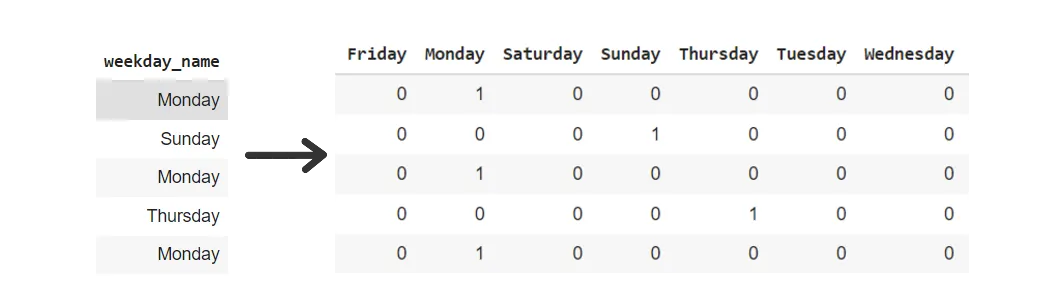
\includegraphics[width=0.75\linewidth]{images/onehotencoding.png}
    \caption{One-hot encoding sample illustration \cite{onehotencoding}}
    \label{fig:one-hot}
\end{figure}

\subsection{Data scaling}

Data scaling is the process of \textbf{adjusting the range of values} in a dataset to ensure that all variables contribute equally to the analysis. It prevents certain features from dominating others due to differences in their scales. Common scaling techniques include Min-Max scaling, where values are normalized to a specific range, and Z-score normalization (formula found in figure \ref{eq:standardization}), which standardizes data to have a mean of 0 and a standard deviation of 1. The latter is used in this work.

\begin{figure}
\[ z_{ij} = \frac{{x_{ij} - \bar{x}_j}}{{\sigma_j}} \]
\caption{Z-score normalization formula}
\label{eq:standardization}
\end{figure}
\text{Where:}
\begin{itemize}[noitemsep, leftmargin=*]
  \item[] $z_{ij}$ \text{ is the normalized value in the } i\text{-th row and } j\text{-th column.}
  \item[] $x_{ij}$ \text{ is the original value in the } i\text{-th row and } j\text{-th column.} 
  \item[] $\bar{x}_j$ \text{ is the mean of the } j\text{-th column.} 
  \item[] $\sigma_j$ \text{ is the standard deviation of the } j\text{-th column.}
\end{itemize}


\paragraph{}Z-score normalization brings several benefits to the training of deep learning models. First and foremost, it promotes convergence by accelerating the optimization process. Normalizing features to a common scale enables the model to navigate the parameter space more efficiently, facilitating \textbf{faster convergence} during gradient-based optimization.

Additionally, as said, z-score normalization aids in stabilizing the training process by \textbf{preventing certain features }from\textbf{ dominating others}. In datasets with disparate feature scales, the influence of larger magnitude features can overshadow smaller ones. This dominance can lead the model to prioritize certain features, neglecting others and resulting in suboptimal generalization. Z-score normalization mitigates this issue by equalizing the impact of all features.

\subsection{Data augmentation}
\label{subsec:data-augmentation}

Data augmentation is a technique commonly used in deep learning to artificially increase the diversity of a training dataset. The idea is to apply various transformations to the existing training data, creating new, slightly modified versions of the original samples. This process helps the model generalize better to unseen data and improves its robustness.
In the context of this research project, the application of a data augmentation technique known as jittering was examined across three datasets. Jittering involves the introduction of random noise into the time series. Specifically, to each observation, a random value drawn from a Gaussian distribution with a mean of 0 and a standard deviation ranging from 0 to 0.2 was added. Importantly, this standard deviation varied at each epoch during the training process.

\begin{figure}
\[X_{\text{jittered}, i} = X_i + \epsilon_i\]
\label{eq:jittering}
\end{figure}
Where: 
\begin{itemize}[noitemsep, leftmargin=*]
    \item[] $X_{\text{jittered}, i}$ represents the \(i\)-th data point in the jittered time series
    \item[] \(X_i\) is the \(i\)-th data point in the original time series
    \item[] \(\epsilon_i\) is the random noise sampled from a Gaussian distribution
\end{itemize}

\begin{figure}
    \centering
    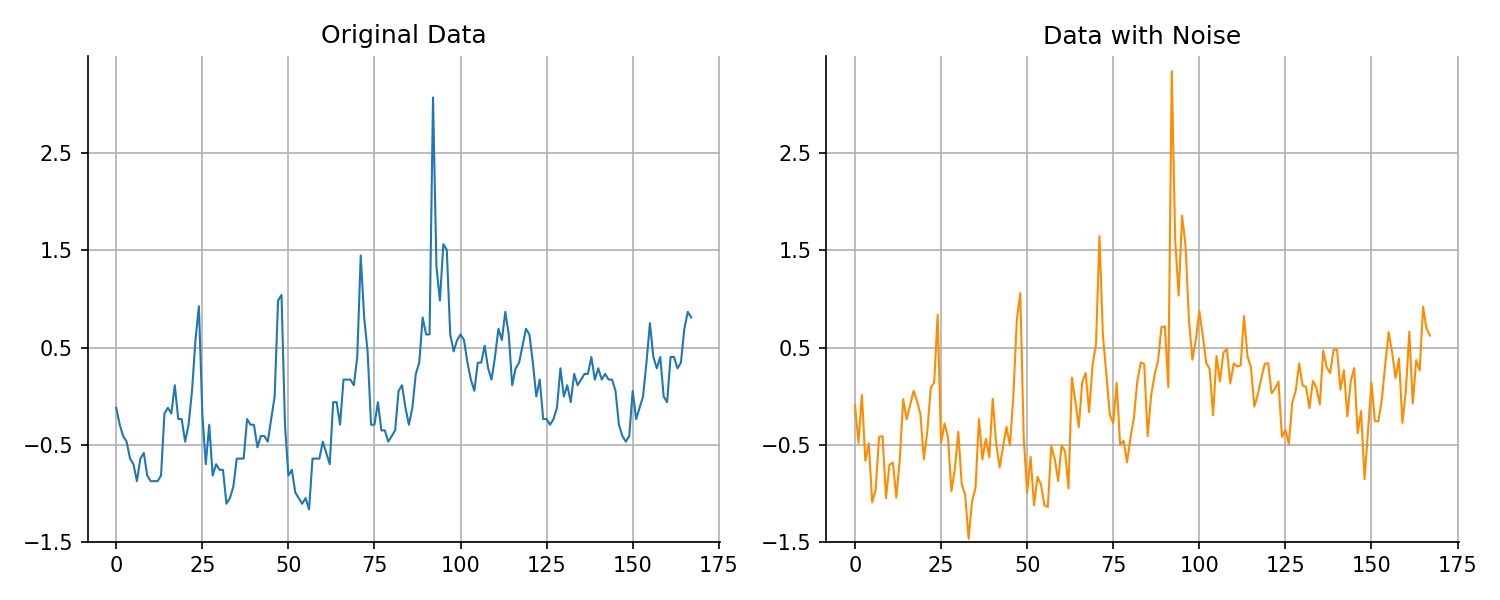
\includegraphics[width=0.75\linewidth]{images/jittering.png}
    \caption{Example of jittering in time series data, with random noise from Gaussian distribution $\mu = 0$ and $\sigma = 0.2$}
    \label{fig:jittering}
\end{figure}


\subsection{Data splitting}

The research question of this work involves a multivariate multi-step forecasting task. In practical terms, this means using past observations at time $t_{past}$ to predict a future time horizon at $t_{future}$. Typically, the time window used for $t_{past}$ is greater than or equal to the time window used for $t_{future}$.
In our case, we employ a technique that transforms the dataset from unsupervised to supervised. A dataset for supervised learning contains one or more target variables, each assigned to a set of independent variables.
In all experiments, we used 168 past observations (24 observations per day for 7 days) to forecast 24 future observations (1 day).

Regarding the data used for model training, it was divided into 3 temporally ordered splits:
\begin{itemize}
    \item Training data (first 80\% of the data)
    \item Validation data (10\% of the data)
    \item Test data (10\% of the data)
\end{itemize}

It is worth noting that for time series forecasting tasks, it is critical that the data sampling for each set is not random, but rather that the data is extracted in chronological order. This is to prevent the model from being exposed to data that will later need to be forecasted in the validation and test sets, ensuring results that are faithful to real-world scenarios.

The introduction of noise in the data takes place online during the training phase, and it is added to each batch individually.

\subsection{Experiments}
\label{subsec:experiments}
While the following section will present the tested models, this section will briefly discuss the examined time horizons. The objective is to assess the effectiveness of the models not only across various cities, each characterized by distinct pollutant distribution patterns, but also in relation to the volume of historical data available. Therefore, the aim is to determine whether and to what extent the possession of more or less historical data influences the accuracy of predictions.

Additionally, the study aimed to assess the effectiveness of the models using both original and noise-augmented data. A summary table of the experiments conducted is presented in Table \ref{tab:dataset_testing}.


\begin{table}[h]
  \centering
  \begin{tabular}{|c|c|c|c|}
    \hline
    \textbf{Dataset} & \textbf{Time Horizon} & \textbf{Original Data} & \textbf{Data with noise} \\ 
    \hline
    Seoul & 1 year & \checkmark &  \\
     & 3 years & \checkmark & \checkmark \\    \hline
    Madrid & 1 year & \checkmark &  \\
     & 3 years & \checkmark & \checkmark \\    \hline
    Citypulse & 3 months & \checkmark & \checkmark \\
    \hline
  \end{tabular}
  \caption{Temporal and Data Variation in Model Testing}
  \label{tab:dataset_testing}
\end{table}

\section{Model architectures}

Deep learning models are known for their complex architectures, which consist of multiple layers and numerous parameters. The interaction of these components can introduce a high degree of variability in the performance of different models, even when they are trained on the same dataset. Therefore, it is essential to use rigorous testing procedures to evaluate the effectiveness of various architectures. Evaluations are based on objective metrics such as error, as well as considerations of generalization and computational efficiency.
Various architectures, from basic to modern, have been tested for their effectiveness, efficiency, and generalization capability.

\subsection{ARIMA}
\label{subsec:baseline}

To provide an overall comparison between the models proposed, an ARIMA model has been developed, which, taking as input one pollutant at once, together with other variables, including the time-based features, predicts the variable for multiple steps over time. 
The Autoregressive Integrated Moving Average (ARIMA) model is a traditional time series forecasting technique developed by Box and Jenkins \cite{box1970time}. It combines autoregression (AR), differencing (I), and moving averages (MA). The general form is ARIMA(p, d, q), where p is the autoregressive order, d is the differencing order, and q is the moving average order. The model equation is the following:
\begin{align*}
(1 - \phi_1 L - \dots - \phi_p L^p)(1 - dL)^d Y_t = c + \theta_1 \varepsilon_{t-1} + \dots + \theta_q \varepsilon_{t-q} + \beta_1 X_{1,t} + \dots + \beta_k X_{k,t}
\end{align*}
Where: 
\begin{itemize}[leftmargin=*, noitemsep]
    \item[] $Y_t$ time series value at time $t$
    \item[] $L$ lag operator, such that $L^k Y_{t-k} = Y_{t-k}$ 
    \item[] $\phi_1, \dots ,  \phi_p$ autoregressive (AR) parameters
    \item[] $d$ is the differencing order (integrated part)
    \item[] $\theta_1, \dots , \theta_q$ moving average (MA) parameters
    \item[] $c$ optional constant term (intercept)
    \item[] $\varepsilon_t$ white noise error term at time $t$
    \item[] $X_{1,t}$, \dots, $X_{k,t}$ are external regressors or exogenous variables at time $t$. 
    \item[] $\beta_1$, \dots, $\beta_k$ are the coefficients associated with the external regressors.
\end{itemize}



ARIMA is a commonly used method for time series forecasting because of its adaptability and interpretability. The model's parameters (p, d, q) are determined through an automated process called auto-ARIMA, which uses algorithmic methods to select the optimal values of p, d, and q based on the minimization of a metric, typically the Akaike Information Criterion (AIC). This automated approach streamlines the model selection process and improves forecasting accuracy.

Additional statistical techniques are available to effectively model data seasonality or employ multivariate modeling. However, these methods fall outside the current scope of the study and will not be examinated.

\subsection{Linear model}

The initial deep learning model used is an MLP (Multi-Layer Perceptron) architecture. It flattens the first dimension in the data and utilizes all observations, ignoring the temporal sequence, and then attempts to output the sequences. This first method is a baseline for all other models based on deep approaches, which will instead preserve the temporal dimension to make multi-step predictions.
To ensure simplicity, no activation function was used for the model weights, resulting in a linear activation function. It should also be noted that despite the simplicity of the design, this is the largest network in terms of the number of parameters and the weight of the model (70-100 million parameters).

\begin{figure}
    \centering
    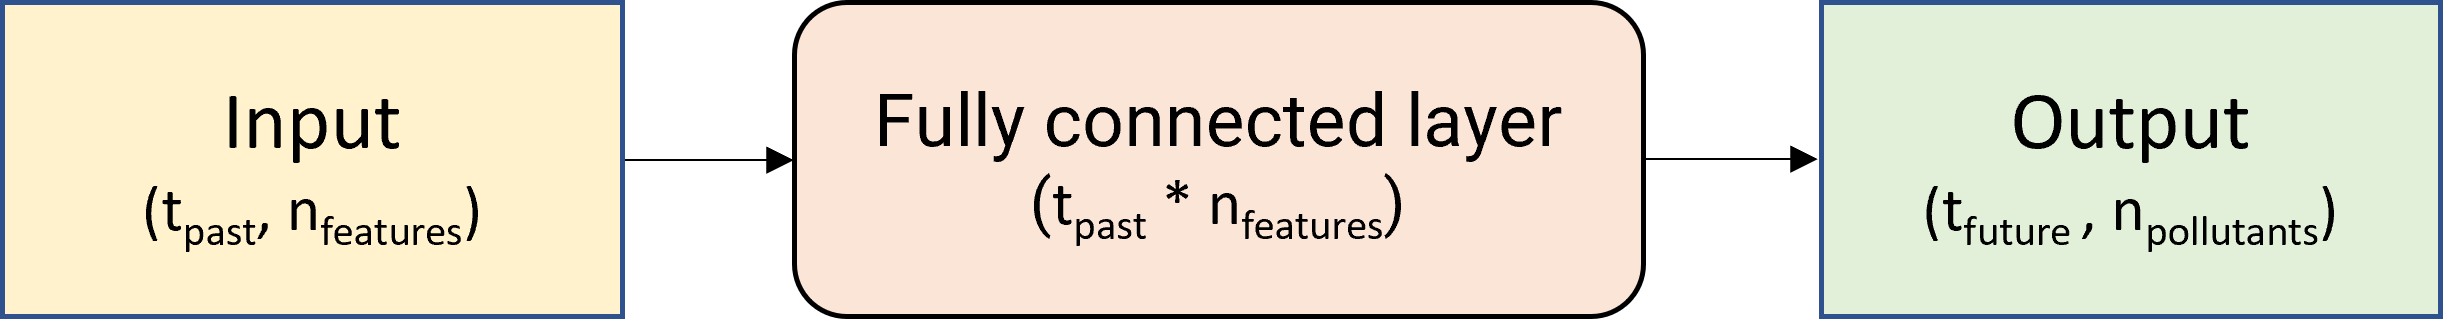
\includegraphics[width=0.7\linewidth]{images/model architectures/linearmodel.png}
    \caption{Proposed linear model architecture. The model takes an input matrix of size t\textsubscript{past} dimensions by features, and employs an MLP with no hidden layers to yield an output matrix sized t\textsubscript{future} dimensions by pollutants.}
    \label{fig:linearmodel}
\end{figure}

\subsection{LSTM model}

LSTMs (Long Short-term Memory) networks were introduced in 1997 by Sepp Hochreiter and Jürgen Schmidhuber \cite{hochreiter}. LSTM networks were created with the explicit purpose of addressing the challenge of long-term dependencies encountered by recurrent neural networks (RNNs), primarily stemming from the \textbf{vanishing gradient problem}\footnote{
In the process of training a recurrent neural network (RNN), the backpropagation algorithm moves in a backward direction from the output layer to the input layer. However, a common issue arises during this progression known as the \textbf{vanishing gradients problem}. As the algorithm descends, the gradients tend to diminish and become shallower, approaching zero. This phenomenon has a significant impact on the weights of the initial or lower layers, rendering them nearly unchanged. Consequently, the gradient descent optimization struggles to converge to the optimum solution. }. Distinguishing themselves from conventional feedforward neural networks, LSTMs incorporate feedback connections. This unique attribute empowers LSTMs to analyze entire sequences of data, such as time series, in a manner that goes beyond treating each point in the sequence in isolation. Instead, LSTMs retain valuable information from preceding data points in the sequence, facilitating the handling of new data points. Consequently, LSTMs excel in processing sequential data, making them particularly effective for tasks involving text, speech, and general time-series analysis.
The proposed model comprises two LSTM layers, each consisting of 50 LSTM units, arranged in a stacked configuration, wherein the output of the first layer serves as the input to the second. This architectural arrangement confers advantages by facilitating the acquisition of hierarchical representations of successive observations and enabling the detection of latent patterns within the data. Dropout regularization is applied following both LSTM layers, employing a rate of 0.4. Dropout is a regularization technique that stochastically sets input units to zero with a specified frequency (0.4 in this instance) during each training iteration, mitigating the risk of overfitting.
The output of the second LSTM layer yields, for each sample within the batch, a feature vector of dimensions 50. Subsequently, this feature vector is supplied to a dense linear layer for predictive modeling.

\begin{figure}
    \centering
    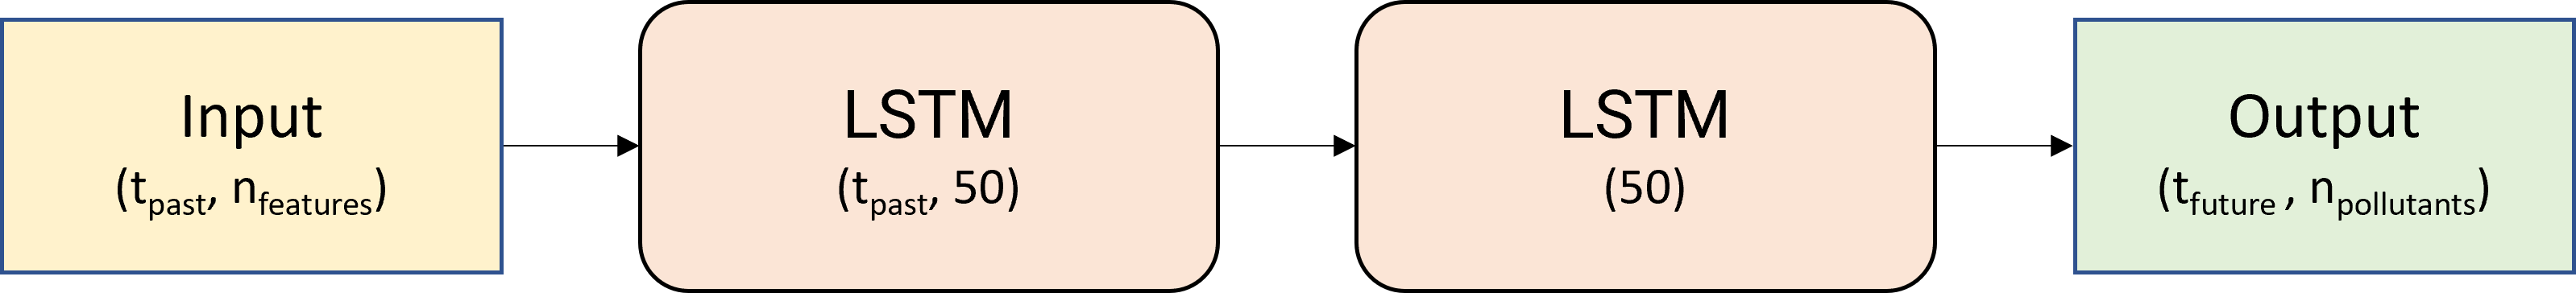
\includegraphics[width=0.7\linewidth]{images/model architectures/lstmmodel.png}
    \caption{Proposed LSTM model architecture. It involves processing an input matrix of size $t_{\text{past}}$ by features through two LSTM layers. The first LSTM layer generates an array of size 50 for each past time step, and the second LSTM layer produces a single feature vector of size 50. This vector is then passed to a dense linear layer, resulting in an output matrix of dimensions $t_{\text{future}}$ by pollutants.}
    \label{fig:lstmmodel}
\end{figure}

\subsection{Bidirectional LSTM model}


Bi-LSTM, short for Bidirectional Long Short-Term Memory, represents a variant of recurrent neural networks (RNNs) designed to effectively handle sequential data by processing it in both forward and backward directions.
The bidirectional processing of Bi-LSTM stands in contrast to one-directional processing in traditional RNNs \cite{Schuster1997BidirectionalRN}. Comprising two LSTM layers, one for forward and one for backward processing, each layer maintains its distinct hidden states and memory cells.
The forward pass involves feeding the input sequence into the forward LSTM layer, updating hidden states and memory cells at each time step based on current input and past information. Simultaneously, the backward pass processes the input sequence in reverse order, updating hidden states and memory cells based on current input and future context. After both passes, the hidden states from both LSTM layers are combined at each time step, enhancing the model's ability to capture comprehensive dependencies.

The proposed model is similar to the previous one, with the only difference being in the number of LSTM units in each layer (32 in the first one, and 64 in the second one), and the impementation of bidirectional processing in the two LSTM layers.

\begin{figure}
    \centering
    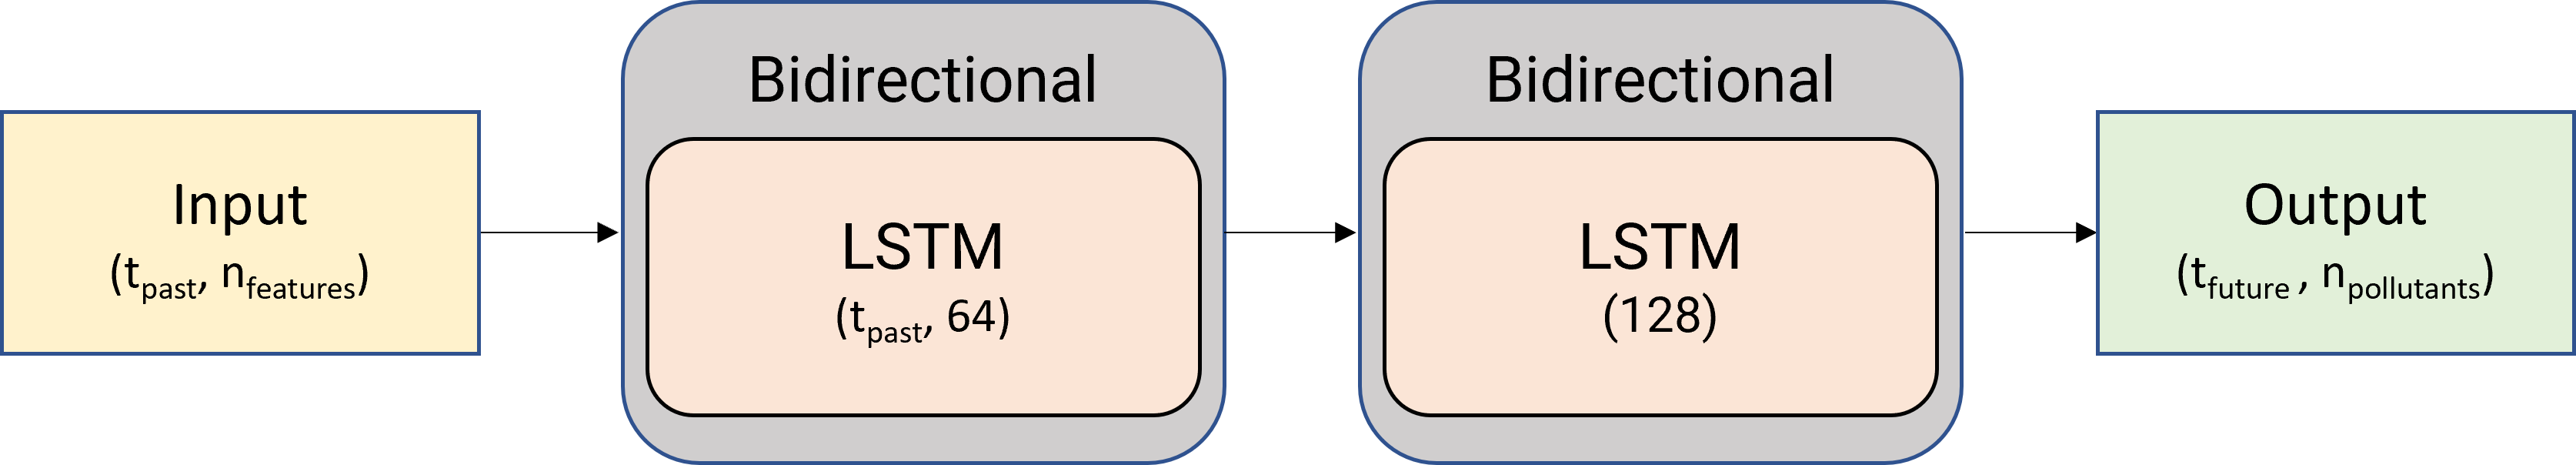
\includegraphics[width=0.7\linewidth]{images/model architectures/bilstmmodel.png}
    \caption{Proposed Bi-LSTM model architecture. It processes an input matrix of size $t_{\text{past}}$ by features, followed by two Bidirectional LSTM layers, first yielding a matrix of size $t_{\text{past}}$, 64, and the second one returning an array of size 128. Then the array is fed to a dense linear layer for predictions.
    }
    \label{fig:bilstmmodel}
\end{figure}

\subsection{Dense Encoder Decoder model}

The model is an autoencoder designed for sequential data. It consists of two blocks, encoder and decoder, each made only of dense layers.

\paragraph{Encoder Layers}
The encoder is responsible for transforming the input data into a more compact representation, often referred to as a latent space or encoding. It performs dimensionality reduction and extracts important features from the input. In the proposed model architecture, the encoder consists of several dense layers with non-linear activation functions (ReLU) and dropout layers. The final output of the encoder is a flattened representation that captures essential features of the input.
\begin{itemize}[noitemsep]
  \item Dense layer (128 units, ReLU activation)
  \item Dense layer (64 units, ReLU activation)
  \item Dense layer (32 units, ReLU activation)
\end{itemize}

\paragraph{Decoder Layers}
The decoder is tasked with reconstructing the original input data from the compressed representation generated by the encoder. It takes the encoded representation and transforms it back into the original format. In the model, the decoder comprises additional dense layers with non-linear activations and dropout layers. The final layer in the decoder produces the output, which is reshaped to match the dimensions of the original input.
\begin{itemize}[noitemsep]
  \item Dense layer (64 units, ReLU activation)
  \item Dense layer (128 units, ReLU activation)
  \item Dense layer (\( t_{\text{future}} \times n_{\text{pollutants}} \), linear activation)
\end{itemize}

\begin{figure}
    \centering
    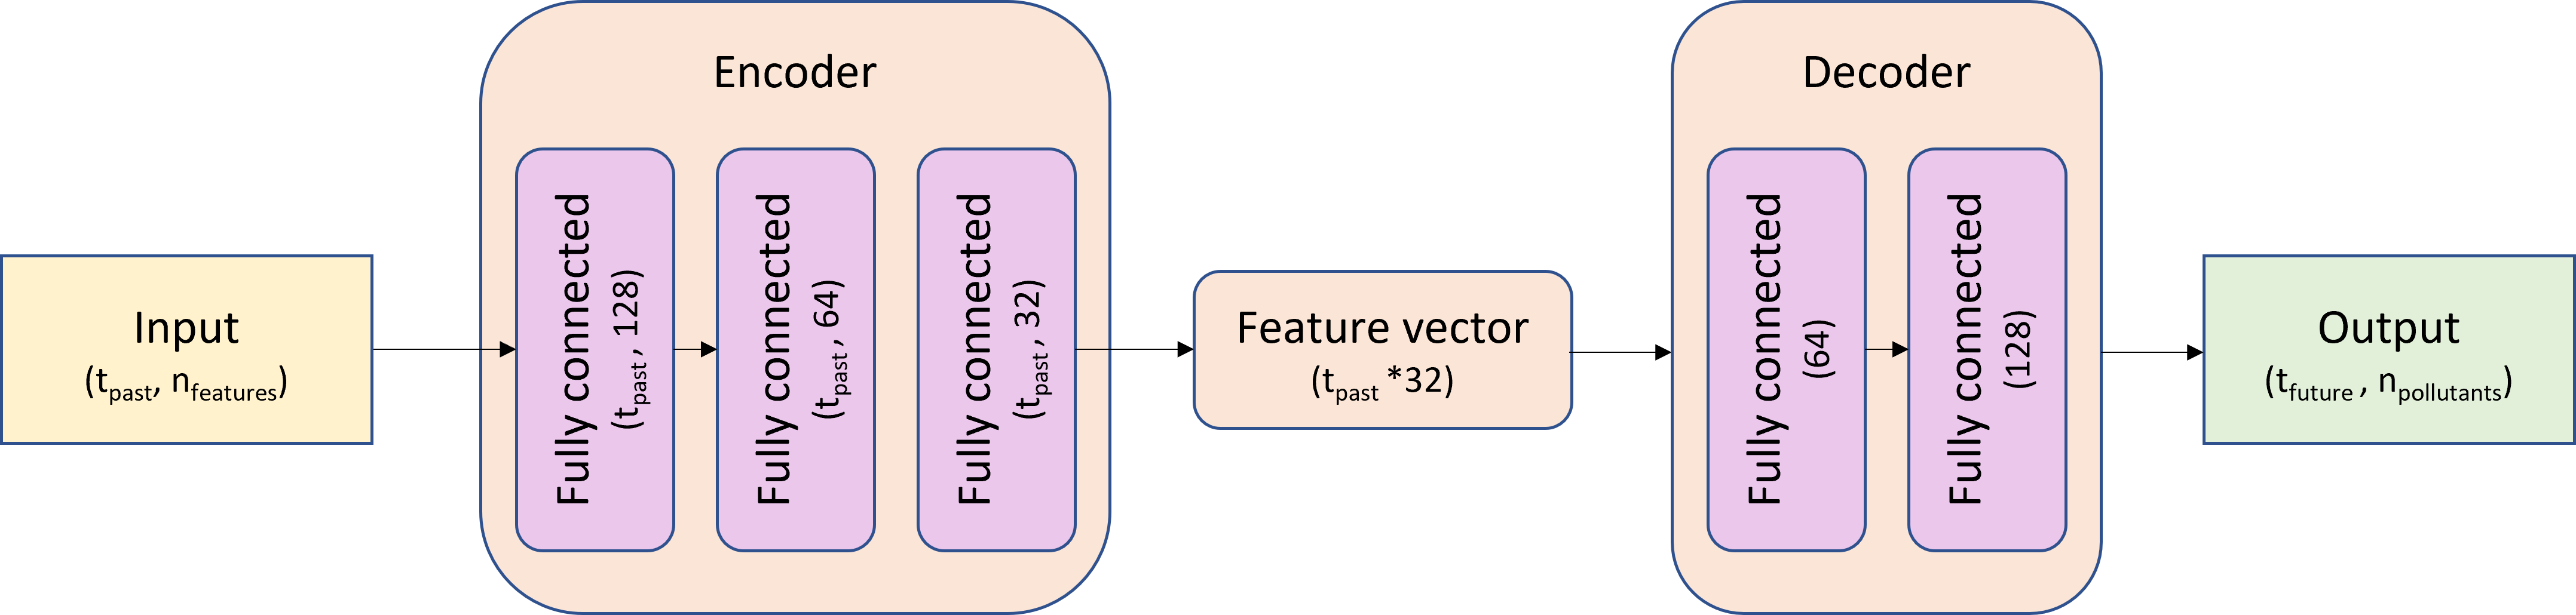
\includegraphics[width=1\linewidth]{images/model architectures/denseencdecmodel.png}
    \caption{Proposed Dense encoder-decoder architecture}
    \label{fig:denseencdecmodel}
\end{figure}

The encoder effectively reduces the dimensionality of the input data, leading to more efficient storage and computation. Additionally, the model is adept at autonomously learning pertinent features from the input data without the need for explicit feature engineering. Dropout layers have been thoughtfully incorporated, serving as a means of regularization to prevent overfitting and augment the model's generalization capabilities.
One notable drawback lies in the fixed architecture of the model, being relatively simplistic and probably unable to adapt dynamically based on the complexity of the data. Another consideration is the potential loss of information during the compression process within the encoding layer. This is particularly relevant if the encoding dimension is too modest, possibly impacting the model's accuracy in faithfully reconstructing the input.

\subsection{CONV-LSTM model}

The proposed model architecture is a combination of Convolutional Neural Network (CNN) and Long Short-Term Memory (LSTM) layers. 
In the initial phase, the model processes input sequences of shape (t\textsubscript{past}, n\textsubscript{features}), where each sequence encapsulates t\textsubscript{past} time steps with n\textsubscript{features} features. The temporal dimension is then divided into seven segments, each representing a day, enabling isolated processing for daily patterns.
For each day, 1D convolutional layers with increasing filter sizes (64, 128, 256). Max pooling and batch normalization follow. Outputs from each day are concatenated along the temporal axis to capture dependencies.
The whole output is then passed through two consecutive LSTM layers, the first with 32 units and dropout (0.4), and the second with 64 units and another dropout layer. The final layer is a dense layer shaped for forecasting.

The combination of CNN and LSTM allows the model to capture both local patterns through convolutional operations and long-term dependencies through LSTM layers. By splitting the input sequence into daily segments, the model may better capture patterns specific to each day, potentially improving performance. Moreover, the use of causal padding in convolutional layers ensures that each output only depends on previous time steps, avoiding information leakage from the future.

However, due to it's complexity, this model could present some drawbacks such as the longer training times and the requirement of a larger amount of data for effective training, together with the risk of overfitting.


\begin{figure}
    \centering
    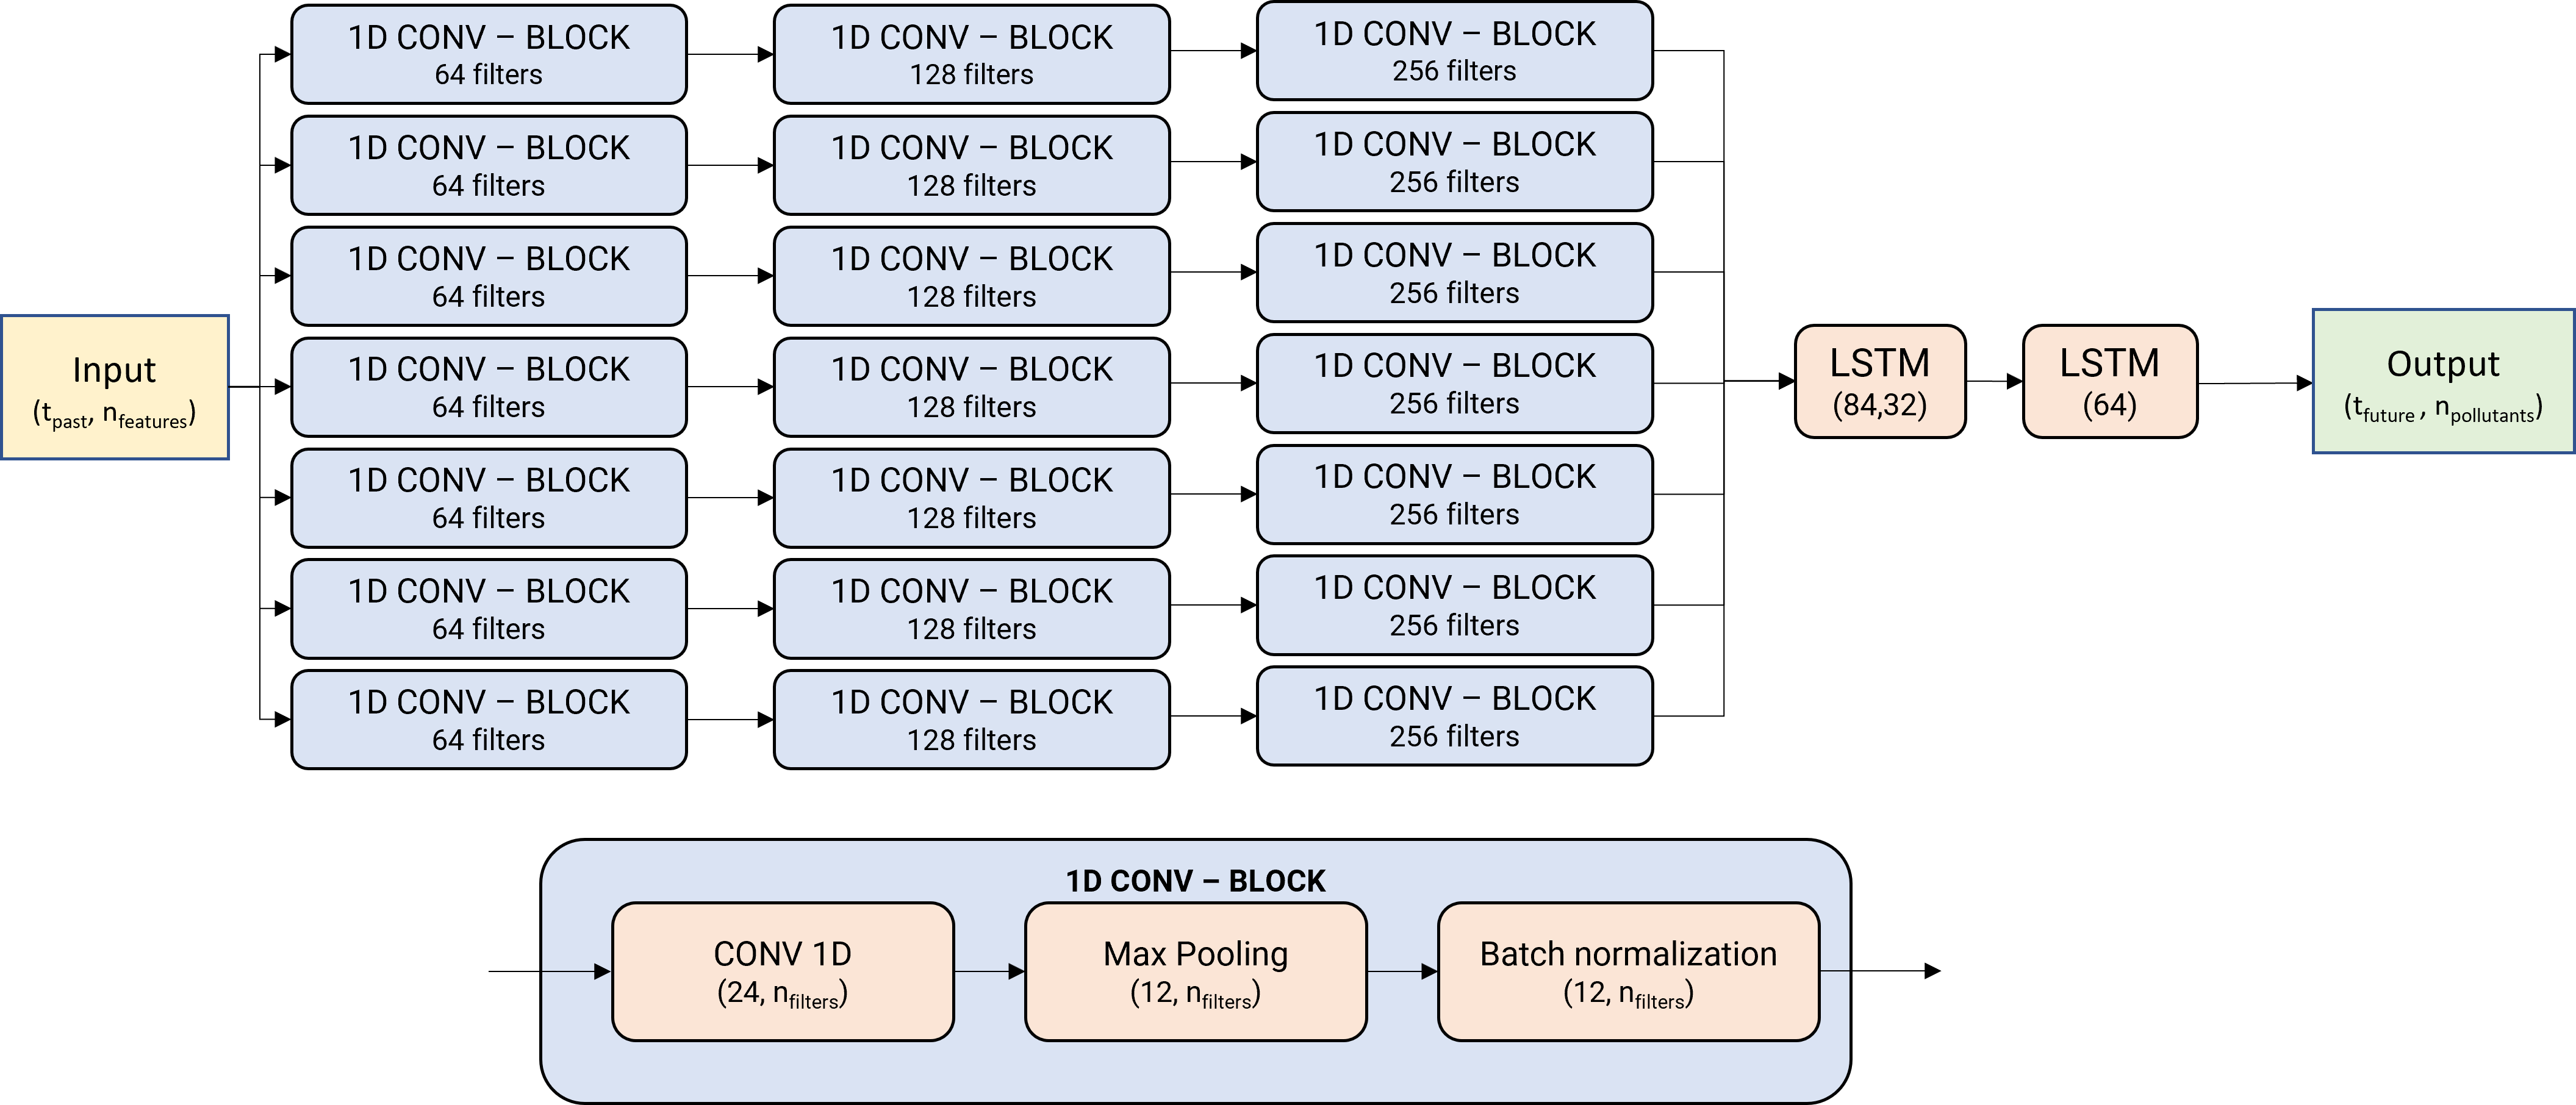
\includegraphics[width=1\linewidth]{images/model architectures/convlstm_model.png}
    \caption{Proposed CONV-LSTM architecture.}
    \label{fig:convlstm_model}
\end{figure}

\subsection{TSMixer model}

TSMixer, an abbreviation for Time-Series Mixer, presents an innovative architecture for time-series forecasting, employing a stacked arrangement of multi-layer perceptrons (MLPs). Documented in the paper entitled "TSMixer: An All-MLP Architecture for Time Series Forecasting" \cite{chen2023tsmixer}, this model diverges from prevailing and conventional methodologies in time-series forecasting. In contrast to contemporary approaches relying on high-capacity architectures like recurrent- or attention-based sequential deep learning models, TSMixer adopts a distinctive strategy by incorporating a sequence of multi-layer perceptrons in its design. The primary focus lies in amalgamating time and feature dimensions to enhance predictive accuracy. This discussion dissects the two principal components of TSMixer.

\paragraph{Mixer Layer}

The Mixer Layer serves as the locus for time mixing and feature mixing, encapsulating the essence of TSMixer's nomenclature.

\begin{figure}
    \centering
    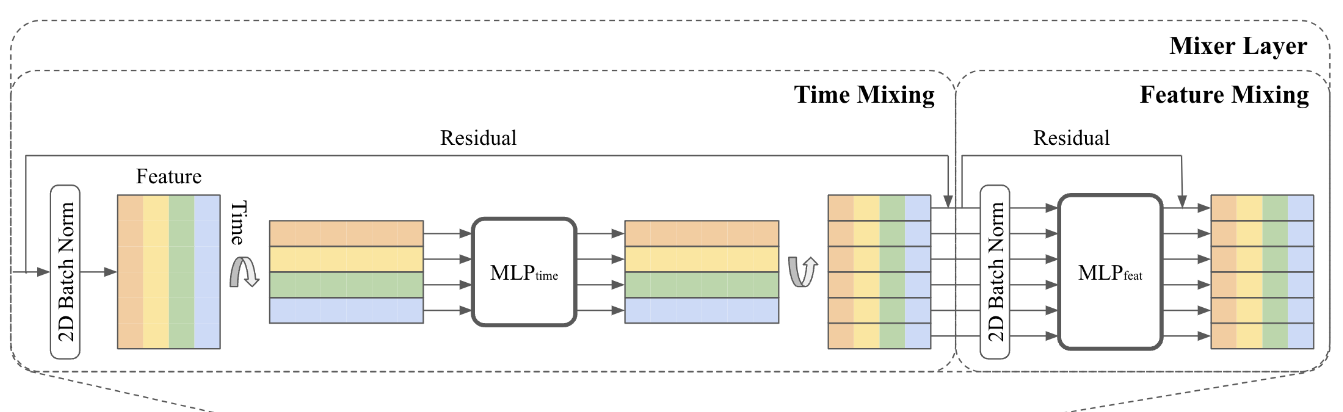
\includegraphics[width=1\linewidth]{images/model architectures/Mixing layer.png}
    \caption{Illustration of the mixing layer. \cite{chen2023tsmixer}}
    \label{fig:tsmixer-mixing-layer}
\end{figure}

The diagram above illustrates the mechanics of time mixing, wherein the MLP encompasses a fully connected layer, followed by the Rectified Linear Unit (ReLU) activation function, and a dropout layer. The input matrix, with rows representing time and columns representing features, undergoes transposition to facilitate the application of the MLP in the time domain, shared across all features. This unit is responsible for learning temporal patterns. Subsequent to exiting the time mixing unit, the matrix undergoes transposition once again before being directed to the feature mixing unit. The feature mixing unit comprises two MLPs and, being applied in the feature domain, is shared across all time steps. Noteworthy is the absence of the need for transposition, as the features are inherently aligned along the horizontal axis. Notably, both mixers incorporate normalization layers and residual connections. The latter aids the model in acquiring more profound representations of the data while maintaining computational efficiency, and normalization proves to be a conventional technique enhancing the training of deep learning models. Upon completion of the mixing process, the output proceeds to the temporal projection stage.

\paragraph{Temporal Projection}

\begin{figure}
    \centering
    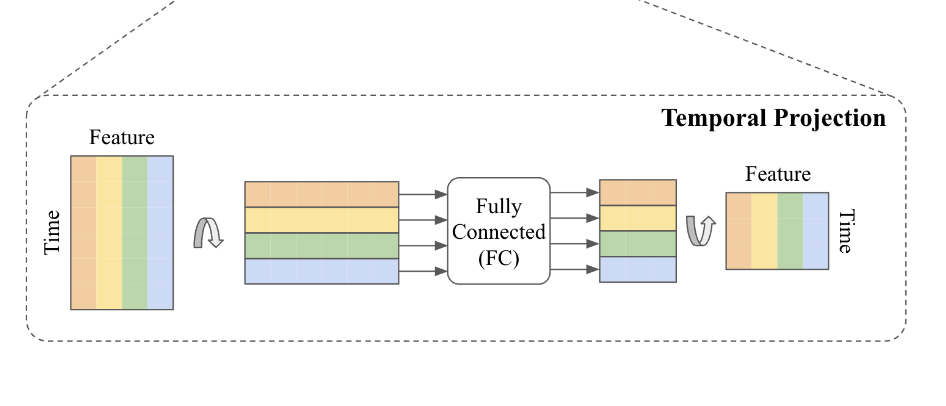
\includegraphics[width=1\linewidth]{images/model architectures/temporalprojection.png}
    \caption{Examination of the Temporal Projection. \cite{chen2023tsmixer}}
    \label{fig:enter-label}
\end{figure}

The Temporal Projection stage involves the retransposition of the matrix, followed by its passage through a fully connected layer to generate predictions. The ultimate step entails retransposing the matrix to arrange the features along the horizontal axis and the time steps along the vertical axis.

\begin{figure}
    \centering
    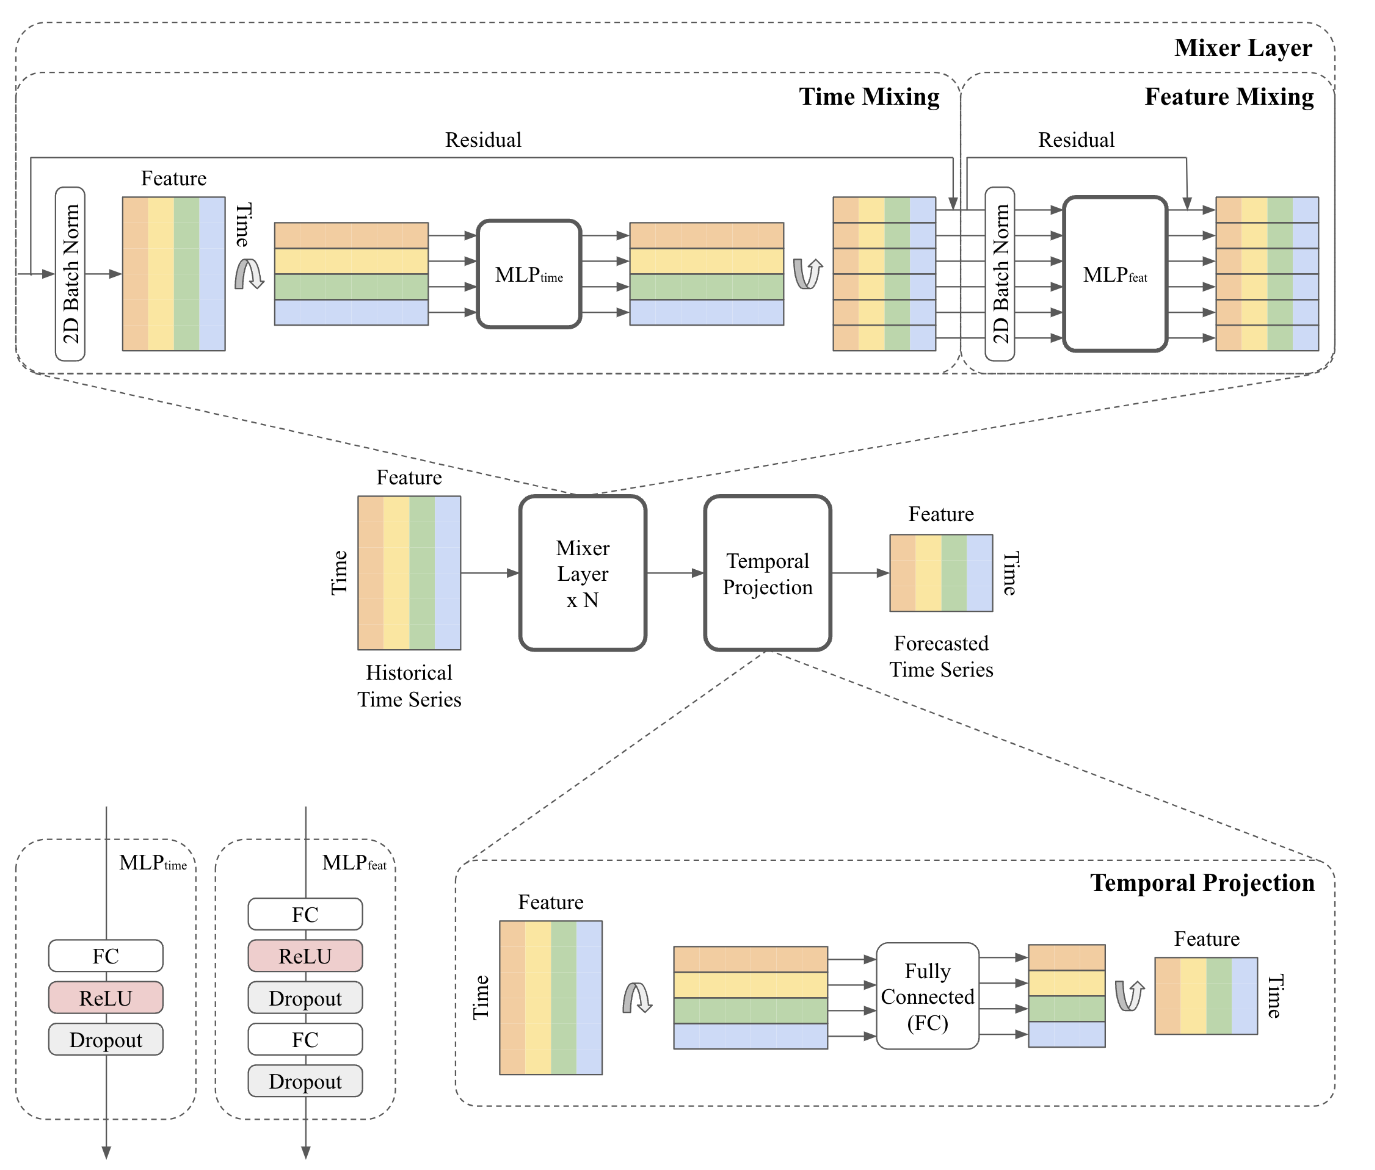
\includegraphics[width=1\linewidth]{images/model architectures/tsmixermodel.png}
    \caption{Comprehensive TSMixer architecture \cite{chen2023tsmixer}}
    \label{fig:tsmixer-whole architecture}
\end{figure}

The incorporation of this model into Tensorflow, covered in the Medium article "TSMixer: The Latest Forecasting Model by Google" \cite{peixeiro2023tsmixer}, enabled the concatenation of 8 mixer layers preceding the temporal projection. This configuration results in heightened complexity, facilitating the capture of intricate patterns within the data. Notably, this heightened complexity does not come with an excessive increase in the number of parameters. Indeed, the model proves to be highly efficient, particularly when compared to the MLP architecture of the linear model.

\subsection{Wavelet model}

The developed wavelet model is a variant of the model proposed in \cite{WaveletNLSTM}. These two model takes advantage of Wavelet transform to decompose the signal into multiple wavelets, processing the components separatedly to capture more hidden patterns between the data.

\textbf{Wavelet transform} is a mathematical tool used for signal processing and analysis. It decomposes a signal into its constituent components called wavelets, which are small, well-localized functions with both time and frequency characteristics. Unlike traditional Fourier transform, which represents a signal as a sum of sinusoids of different frequencies, wavelet transform captures both time and frequency information simultaneously.
The wavelet transform involves passing the signal through a series of filters to extract different frequency components at various scales. The result of this process is a set of coefficients that represent the signal's behavior at different levels of detail and resolution.

In the proposed model, a Daubechies wavelet with one vanishing moment is employed, utilizing three levels of decomposition. The output of the decomposition consists of four arrays of different sizes, which represent the coefficients. These coefficients characterize distinct frequency components and details of the input signal across various scales. The approximation coefficients (cA1) encapsulate the low-frequency components, whereas the detail coefficients (cD1, cD2, cD3) encapsulate the high-frequency details at progressively higher levels of resolution. 


\begin{figure}
    \centering
    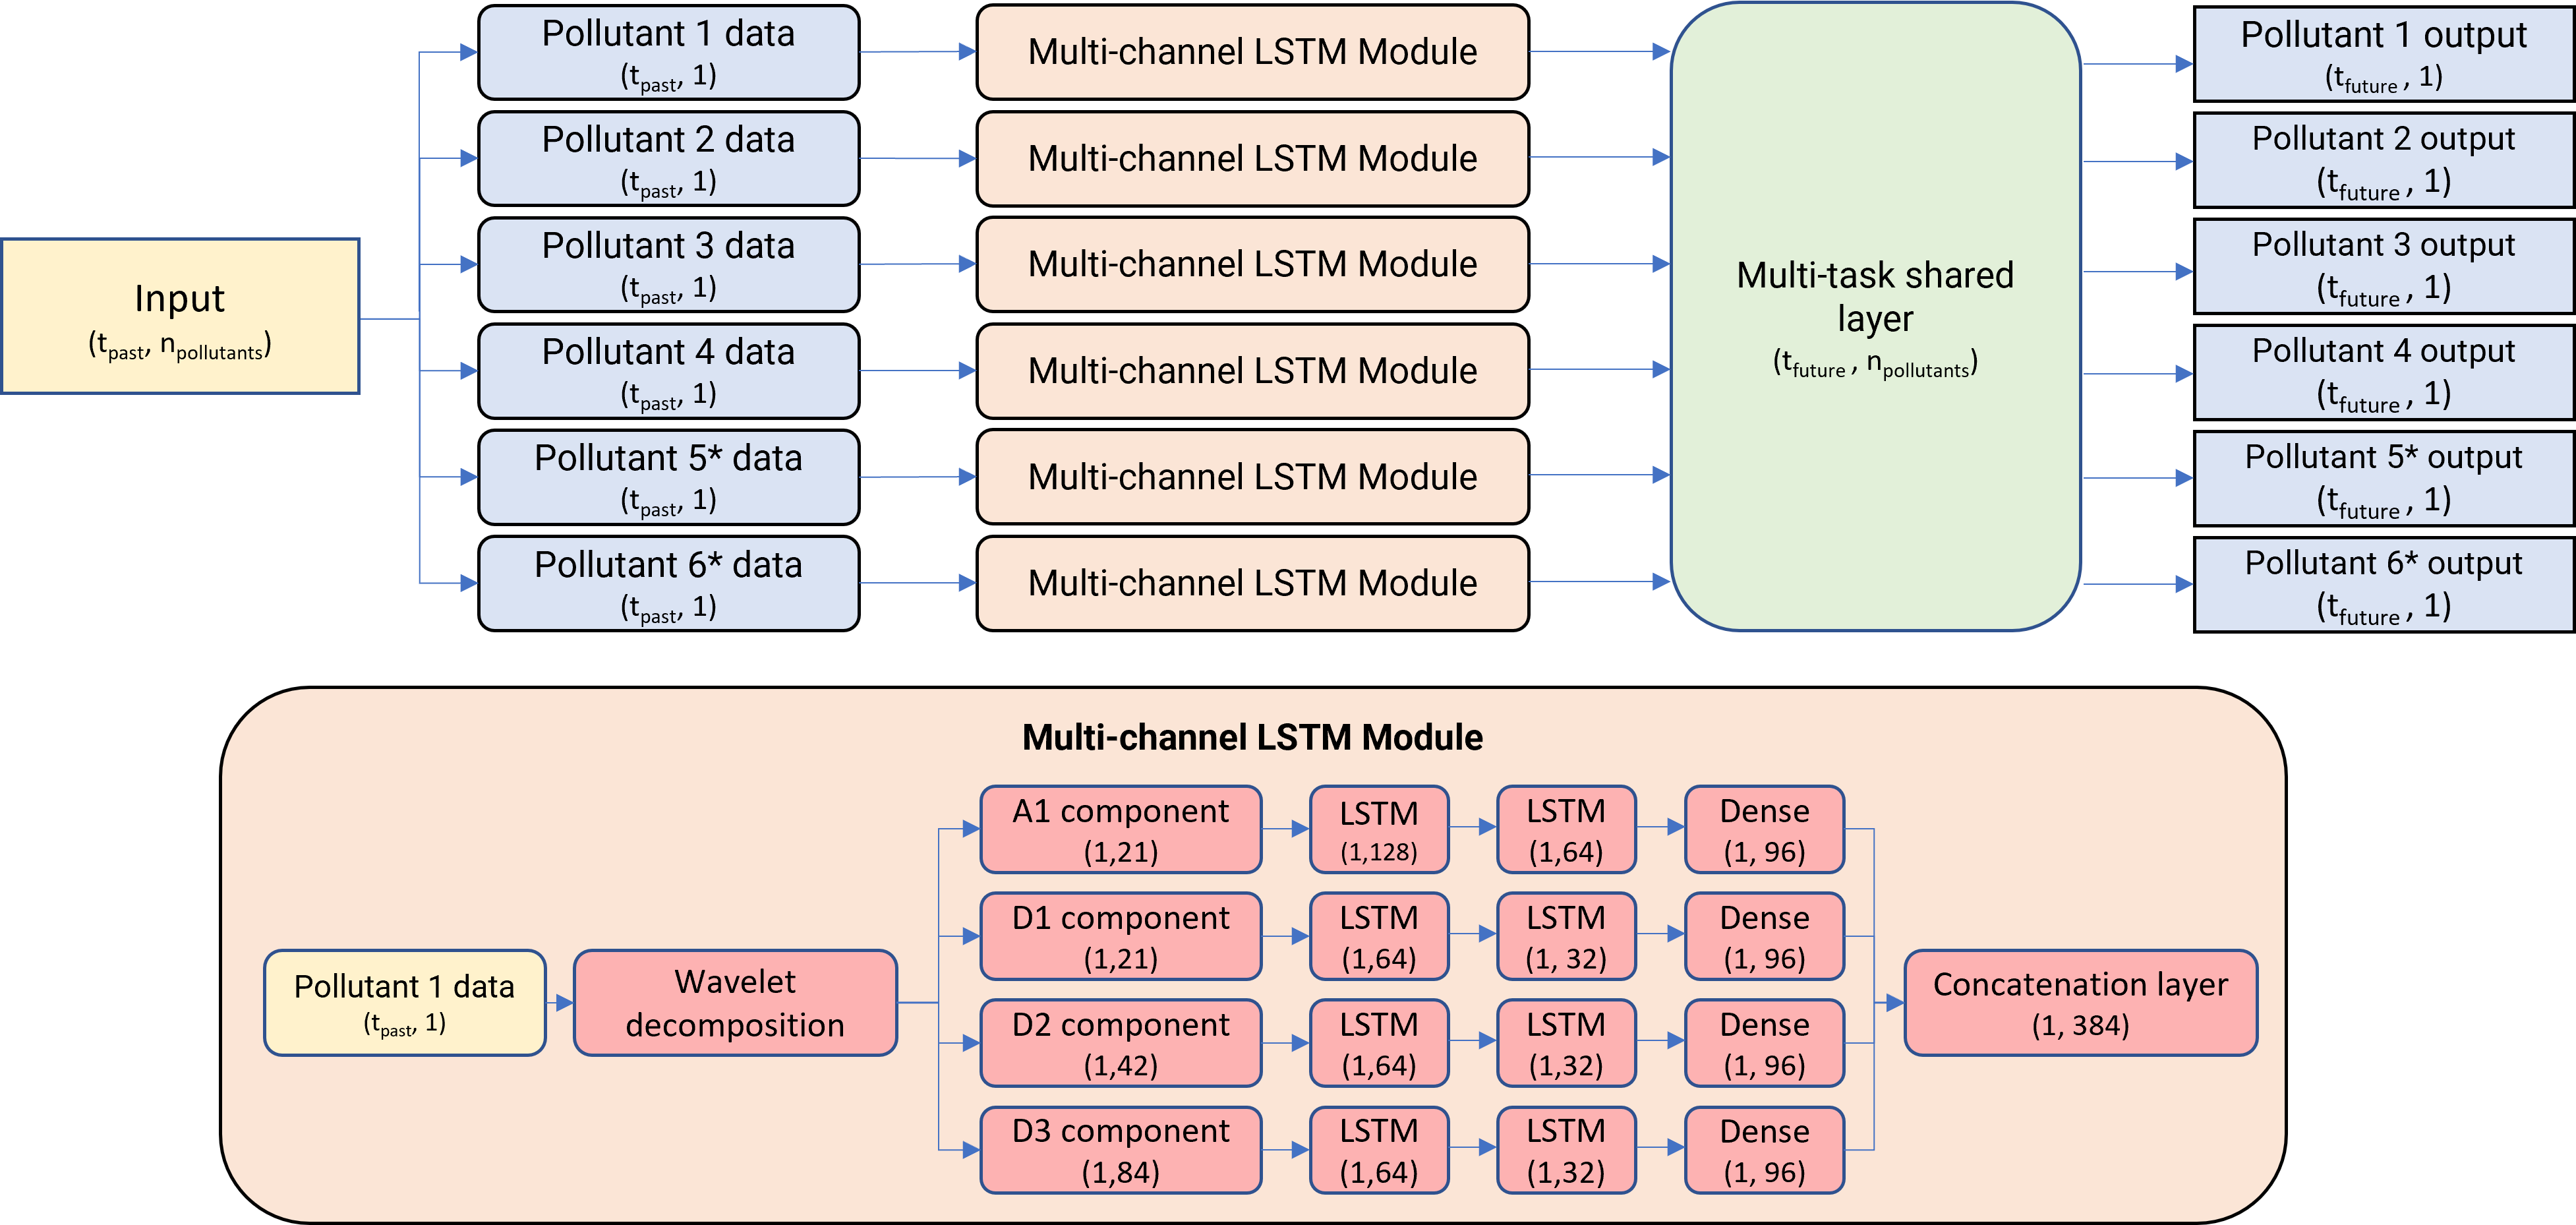
\includegraphics[width=1\linewidth]{images/model architectures/waveletmodel.png}
    \caption{Proposed Wavelet Model architecture}
    \label{fig:waveletmodel}
\end{figure}

The computational focal point is the Multi-channel LSTM module illustrated in Figure \ref{fig:waveletmodel}. Each component undergoes input to two consecutive LSTM layers, followed by processing through a dense layer for the normalization of individual component outcomes. Subsequently, the outputs from each module are consolidated in a shared layer, serving as the basis for the final predictions pertaining to pollutant levels.

\section{Model Evaluation and Training Details}

\subsection{Metrics}

In this section we will shortly present the two metrics utilized to evaluate the performances of the models

\paragraph{Mean Absolute Error (MAE)}
MAE, or Mean Absolute Error, is a metric used to evaluate the accuracy of a forecasting model, particularly in the context of time series forecasting. It measures the average absolute difference between the actual and predicted values, providing a straightforward assessment of the magnitude of errors without considering their direction. In the context of time series forecasting, MAE is useful as it treats underpredictions and overpredictions equally. The formula for calculating MAE is given by:

\[
MAE = \frac{1}{n} \sum_{i=1}^{n} |y_i - \hat{y}_i|
\]

where:
\begin{itemize}[noitemsep, leftmargin=*]
\item[] $n \text{ is the number of observations in the time series,}$
\item[] $y_i \text{ is the actual value at time } i$, 
\item[] $\hat{y}_i \text{ is the predicted value at time } i$.
\end{itemize}

A lower MAE indicates better accuracy, suggesting that the model's predictions are closer to the actual values.

\paragraph{Symmetric Mean Absolute Percentage Error}
When it comes to measuring accuracy relative to the actual values, the most
popular metric is MAPE (the mean absolute percentage error). Whilst being very intuitive MAPE degenerates into positive infinity as soon as any of the actual values is zero. Even relatively small actual values can easily explode MAPE towards infinity. So, effectively, MAPE is meaningful only if all observations have relatively large actual values. 

In this work context, sMAPE is preferred because it addresses the issue of scale, making it suitable for comparing accuracy across different time series with varying levels of magnitude, like ours. Moreover, sMAPE overcomes the MAPE limit of giving different weights in case of overestimation and underestimation. The formula for calculating sMAPE is calculated as follows:

\begin{equation}
sMAPE = \frac{100\%}{n} \sum_{t=1}^{n} \frac{|y_t - \hat{y}_t|}{( |y_t| + |\hat{y}_t| ) / 2}
\end{equation}

where:
\begin{itemize}[noitemsep,  leftmargin=*]
  \item[] \( n \) is the number of observations in the time series.
  \item[] \( y_t \) is the actual value at time \( t \).
  \item[] \( \hat{y}_t \) is the predicted value at time \( t \).
\end{itemize}

The formula calculates the absolute percentage error for each observation in the time series, averages these errors, and then expresses the result as a percentage. The division by \( (|y_t| + |\hat{y}_t|) / 2 \) ensures symmetry in the calculation, emphasizing both overestimation and underestimation errors equally. The sMAPE is expressed as a percentage, but it should not be interpreted as the percentage of the error due to its formulation. A perfect forecast is represented by 0\%, while higher percentages indicate a larger deviation between the actual and predicted values. The sMAPE can reach a maximum value of 200\%, and any value between 100\% and 200\% should be interpreted as an extremely high error.

\subsection{Training configuration}

When defining the training phase, it is important to consider several aspects that can affect the model's performance.
The first aspect to consider is the definition of a \textbf{loss function}. This function is used to update the weights of the neural network during the training phase, with the goal of minimizing or maximizing its value. In this case, we have chosen the \textbf{Mean Squared Error (MSE)} as the loss function. This is calculated by taking the average of the squared differences between the predicted and actual values (see figure \ref{eq:mse}).

\begin{figure}
\[MSE = \frac{1}{n} \sum_{t=1}^{n} (y_t - \hat{y}_t)^2\]
\caption{Mean Squared error formula}
\label{eq:mse}
\end{figure}

where:
\begin{itemize}[noitemsep, leftmargin=*]
  \item[] \( n \) is the number of observations in the time series,
  \item[] \( y_t \) represents the actual value at time \( t \),
  \item[] \( \hat{y}_t \) represents the predicted value at time \( t \), and
  \item[] The summation is taken over all time points from \( t = 1 \) to \( t = n \).
\end{itemize}

The second aspect to consider is the \textbf{optimizer} of the neural network and it's starting learning rate. The optimization algorithm employed in the training of forecasting models is \textbf{Adam} \cite{kingma2017adam}, an abbreviation for Adaptive Moment Estimation. Adam represents an adaptive learning rate optimization algorithm that amalgamates the merits of two well-established optimizers, namely Adagrad and RMSprop. Widely recognized as one of the preeminent optimizers for the training of deep neural networks, Adam is characterized by its capacity to dynamically adjust learning rates for individual parameters. This adaptive characteristic facilitates expedited convergence and enhanced optimization outcomes in practical applications. Adam's adaptability makes it ideal for tasks with fluctuating gradient magnitudes, helping to alleviate challenges such as vanishing or exploding gradient problems commonly encountered in deep learning. The optimal \textbf{learning rate} for all networks during testing was \textbf{0.001}.

To improve efficiency and monitoring during training, various \textbf{callbacks} were implemented:

\begin{itemize}
    \item \textbf{Plot Learning}: Visualizing learning through plots helps understand the evolution of a model. Learning curves, one for training and validation loss, and another one for training and validation MAE, provide insights into performance and identify issues like overfitting or underfitting.

    \item \textbf{Reduce Learning Rate on Plateau}: Dynamic adjustment of the learning rate during training enhances model convergence. This technique involves monitoring a metric (validation loss), reducing the learning rate by a factor of 0.8 if there's no improvement for 3 consecutive epochs, allowing delicate parameter fine-tuning and potential escape from local minima.

    \item \textbf{Early Stopping}: A regularization technique, early stopping halts training when a model's performance on a validation set degrades. Instead of a fixed number of epochs, training stops when there's no further improvement in the validation loss for 5 epochs, preventing overfitting and conserving computational resources.
\end{itemize}
\chapter{Experimental results and discussion}
\label{chap:results}

In this final chapter, we will present and discuss the results obtained through the analysis of various metrics. Initially, we will present the outcomes of all models generated in the conducted experiments (see Section \ref{subsec:experiments}), followed by a more detailed analysis of the top-performing models. 
Furthermore, qualitative representations of predictions will be showcased to enhance the understanding of the models' behavior.



\section{Performances on the test set}
The various configurations of the datasets (see Table \ref{tab:dataset_testing}) have been used to test the models performances.
In this section, with the help of plots, we will analyze the MAE on the test set, dividing it by pollutant, in order to better understand which pollutants' behaviours were better learned  by the models. To evaluate MAE and sMAPE, predictions and the target variables have been rescaled to the original scale.

\subsection{Citypulse}

Of course, as we would expect, results in Citypulse dataset for Ozone and PM\textsubscript{2.5} are almost identical for all models.
Overall (see Figure \ref{fig:aarhus_results}), the most performing models seem to be both LSTMs models, the Dense Encoder Decoder Network, and the Wavelet and TSMixer models. 


\begin{figure}[h]
    \centering
    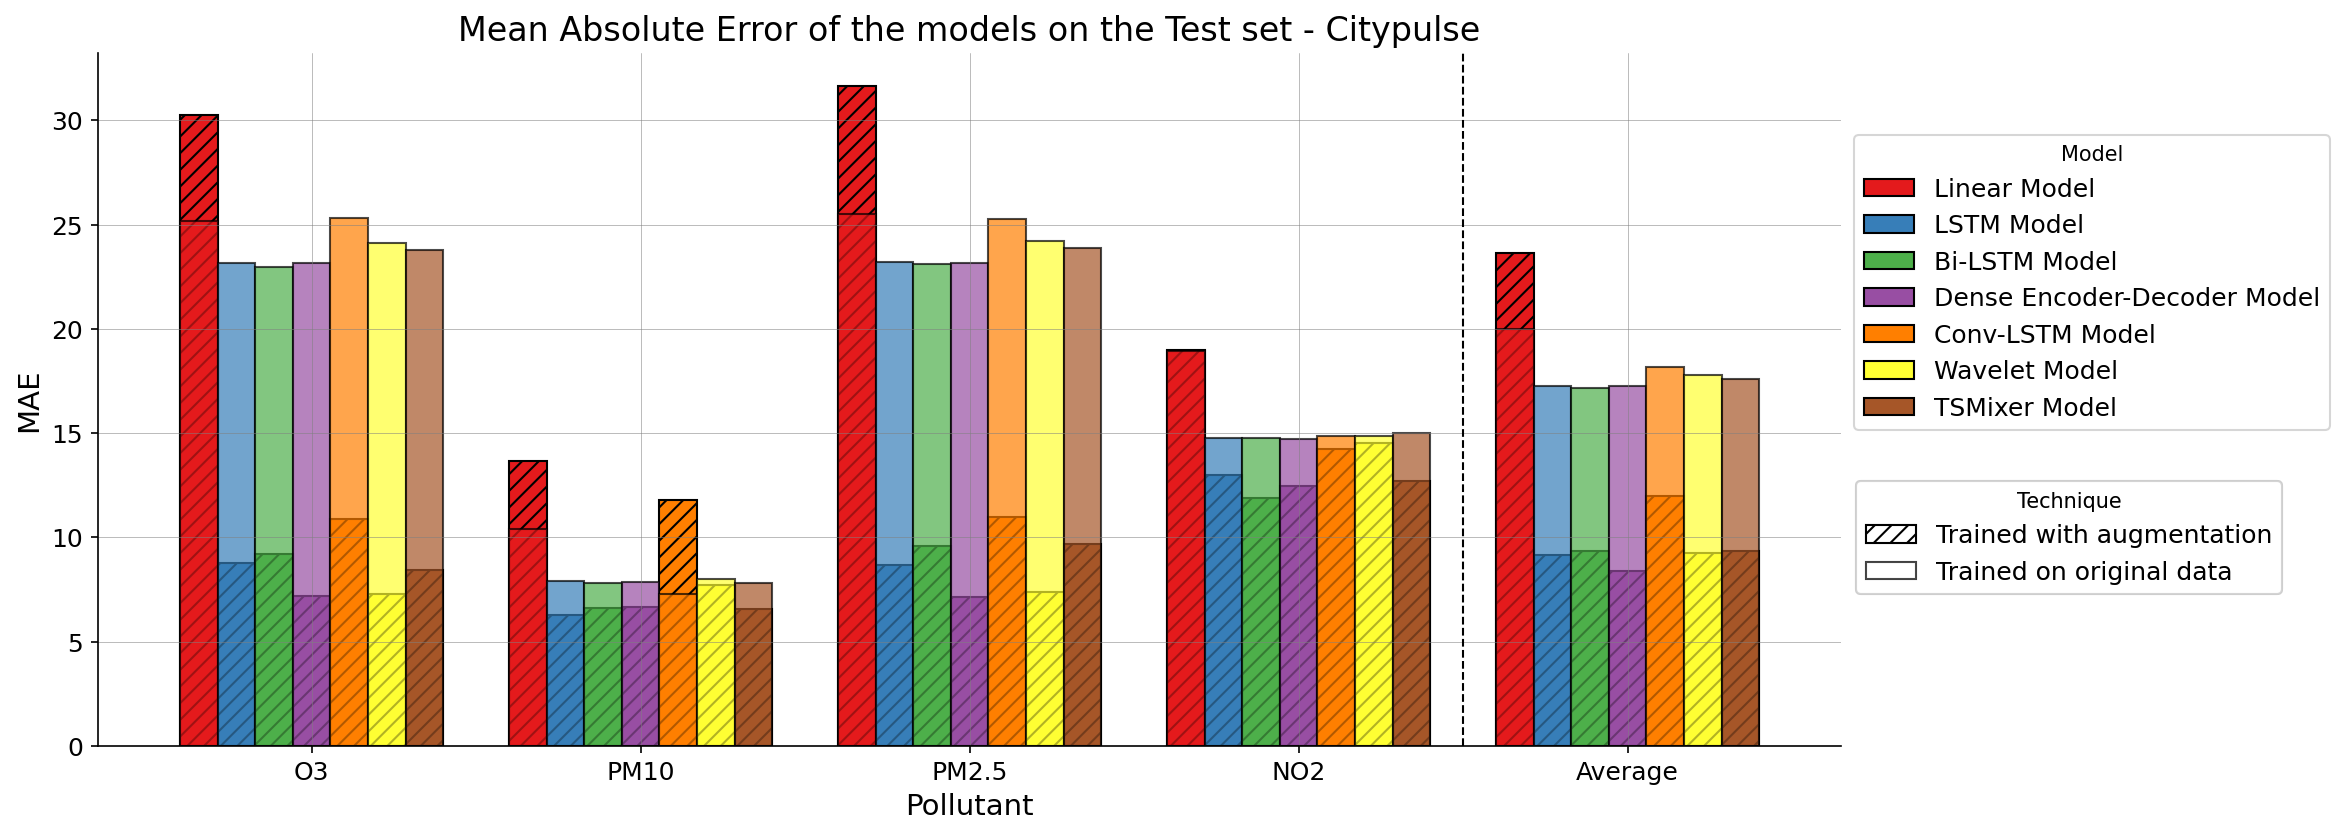
\includegraphics[width=1\linewidth]{images/Aarhus_results.png}
    \caption{MAE on test set, for each model, divided by pollutant. The rightmost graph shows the average MAE of pollutants for each model. Hatched bars represent results after training with augmented data, while solid bars represent MAE without augmented data.}
    \label{fig:aarhus_results}
\end{figure}

It is noteworthy that the linear model does not benefit from the augmentation, exhibiting a higher MAE for all pollutants. This can be attributed to the model's simplicity, as it is unable to adapt to the varying noise injection across epochs and generalize predictions. On average, all models except the linear one yield similar results without augmentation. However, augmentation reveals small differences in the results, but since they are below 1 MAE, it's not enough to select the optimal model for this dataset.
Another aspect that could be noted is that NO\textsubscript{2} and PM\textsubscript{10} presents little differences in MAE in two modalities of training, which could indicate a better predictability of the series.

\begin{table}[h]
    \centering
    \begin{tabular}{lcc}
        \toprule
        \textbf{Model} & \textbf{MAE} & \textbf{sMAPE} \\ 
        \midrule
        Linear & 23,65 & 53.56\% \\
        LSTM & 9,18 & 27.94\% \\
        Bi-LSTM & 9,33 & 27.71\% \\
        \textbf{Dense encoder decoder} & \textbf{8,38} & \textbf{26.38}\% \\
        CONV-LSTM & 11,97 & 34.76\% \\
        TSMixer & 9,34 & 27.81\% \\
        Wavelet & 9,23 & 28.7\% \\ 
        \bottomrule
        \end{tabular}
        \caption{Citypulse models average performances, on augmented dataset models.}
        \label{tab:Citypulse performances}
\end{table}


Ozone and PM\textsubscript{2.5} predictions instead benefits a lot of the augmentation technique. There are two possible explanations for this behaviour:
\begin{enumerate}
    \item The \textbf{collinearity} between the variable is quite reduced by the noise injection, facilitating the models in the prediction task.
    \item Minimizing the loss function could be tricky as each series is independent, and the neural network could focus on minimizing the error for some series, and not improving the others. The noise injection could effectively help the training process in addressing this issue. By introducing controlled random variations or perturbations into the training data through noise injection, the neural network becomes less prone to overfitting on specific series and is better equipped to generalize across diverse sequences.
\end{enumerate}

\subsection{Seoul}

The Seoul dataset yields the best overall results for all models (see Figure \ref{fig:seoul_results}). This is likely due to its consistent observations over time and continuous sensor operation without the need for imputing missing data.

\begin{figure}[h]
    \centering
    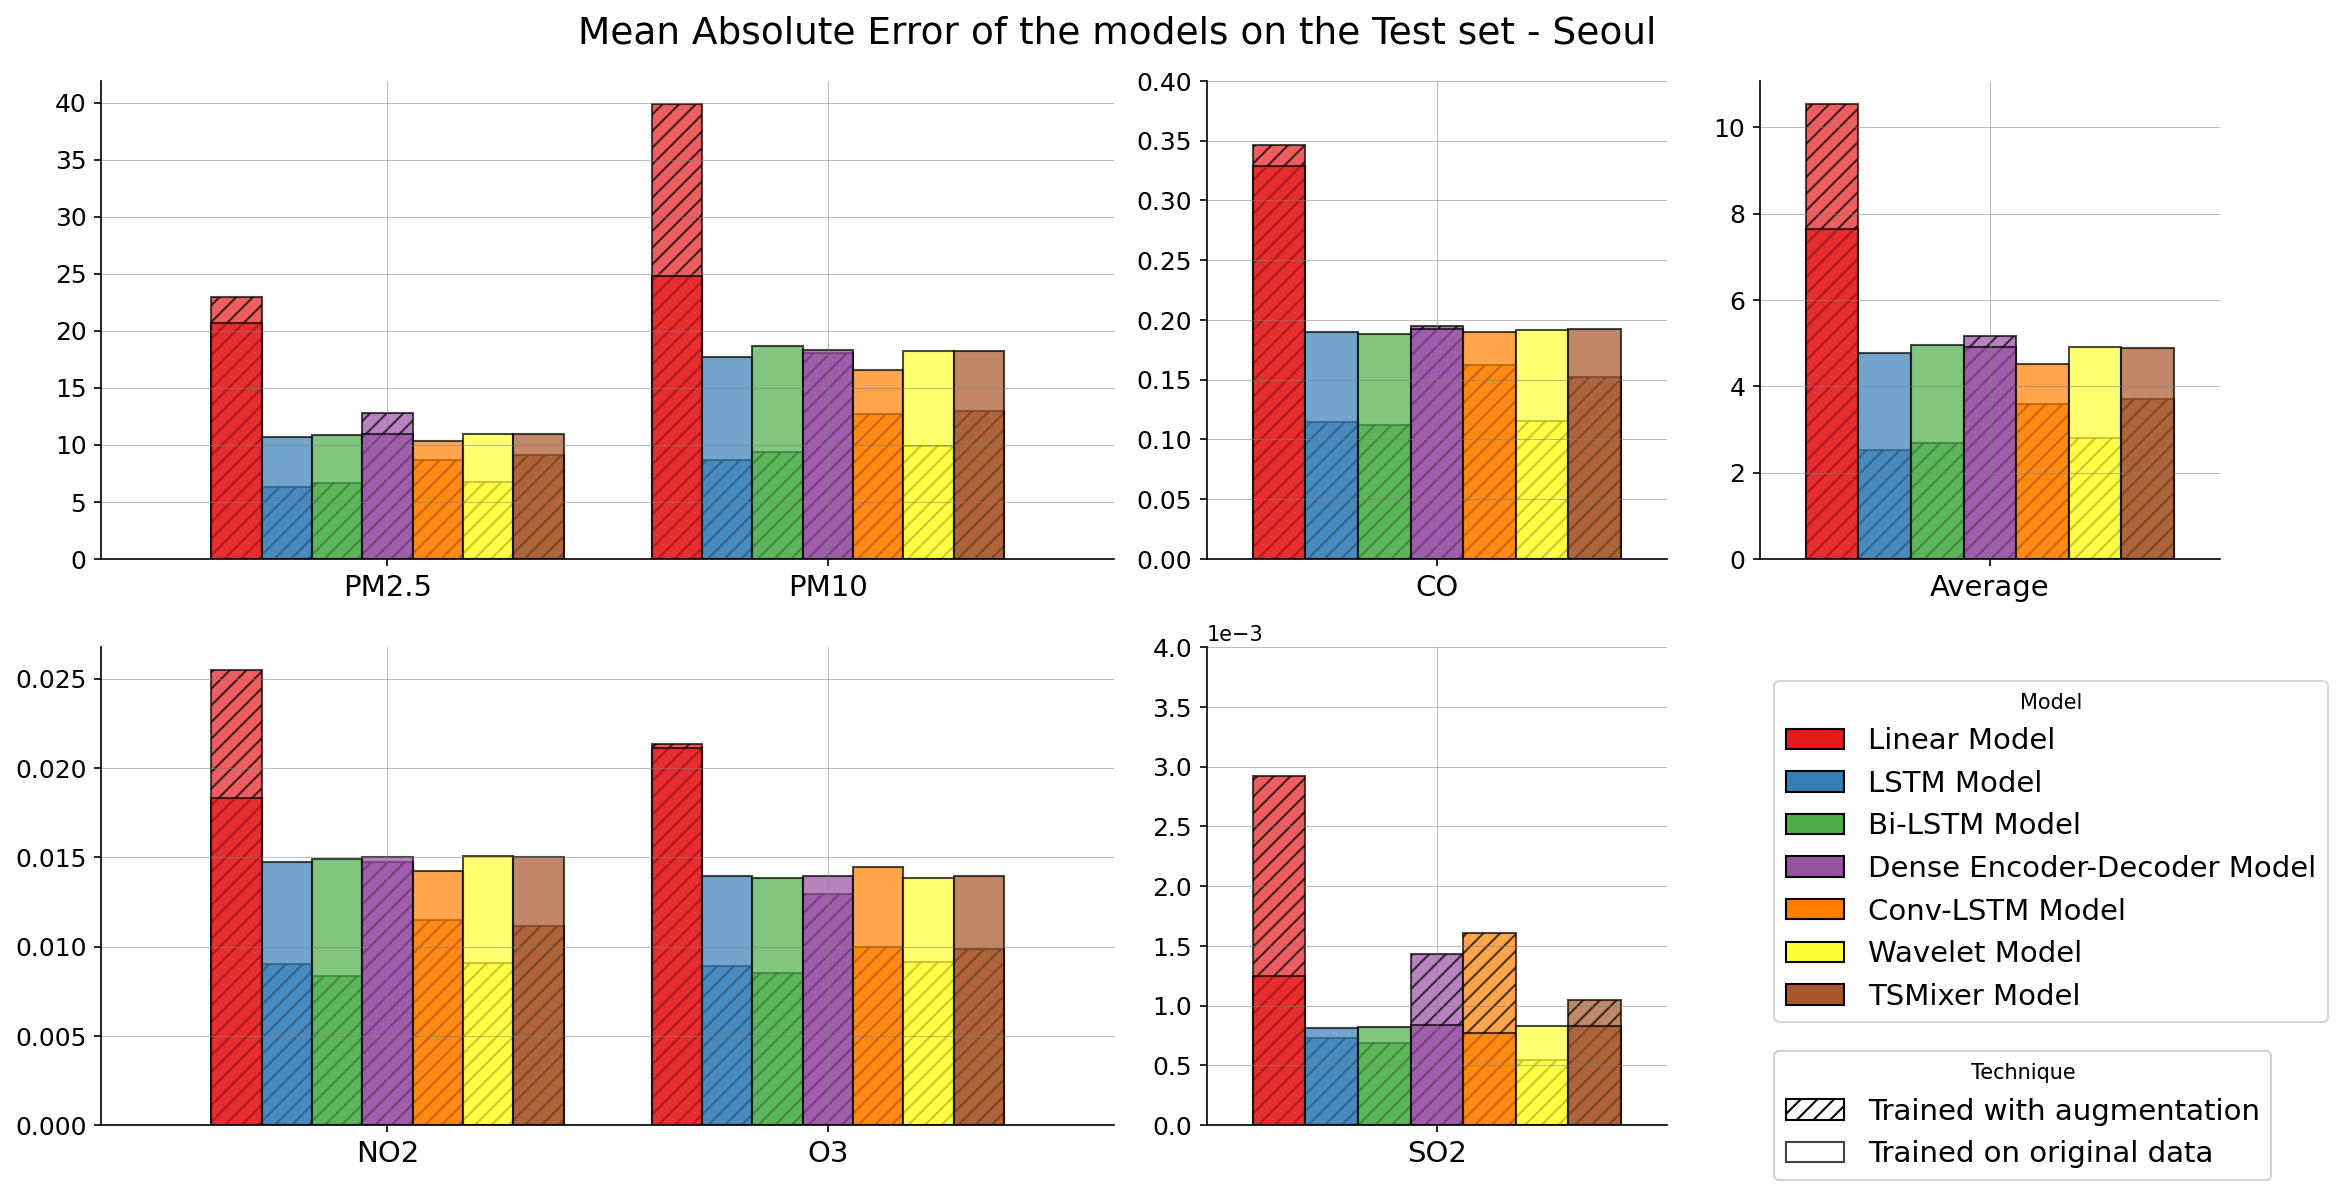
\includegraphics[width=1\linewidth]{images/Seoul_results.png}
    \caption{MAE on test set, for each model, divided by pollutant. The rightmost graph shows the average MAE of pollutants for each model. Hatched bars represent results after training with augmented data, while solid bars represent MAE without augmented data.}
    \label{fig:seoul_results}
\end{figure}

The minimum average MAE encountered is 2.51, in the LSTM model, as we can see in Table \ref{tab:Seoul performances}.
The LSTM, Bi-LSTM, and Wavelet models are the top performers, with a MAE of under 3 and a sMAPE of around 33\%. This is a favorable outcome for real-world applications.

\begin{table}[h]
    \centering
    \begin{tabular}{lcc}
        \toprule
        \textbf{Model} & \textbf{MAE} & \textbf{sMAPE} \\ 
        \midrule
        Linear & 10.55 & 96.93\% \\
        \textbf{LSTM} & \textbf{2.51} & \textbf{33.49}\% \\
        Bi-LSTM & 2.68 & \textbf{33.49}\% \\
        Dense encoder decoder & 5.17 & 51.95\% \\
        CONV-LSTM & 3.60 & 44.18\% \\
        TSMixer & 3.71 & 41.58\% \\
        Wavelet & 2.80 & 33.68\% \\
        \bottomrule
    \end{tabular}
    \caption{Seoul models average performances, on augmented dataset models.}
    \label{tab:Seoul performances}
\end{table}

The linear model exhibits a comparable pattern to the one found in the Citypulse data, which emphasizes its limitations. Despite achieving satisfactory results even in the absence of augmentation, attributed to the substantial volume of training data, the introduction of augmentation enhances performance by an additional 2 points across the top-three models. This reaffirms the potential of augmentation, even in scenarios where ample training data is already available.
Unlike to what is seen in Aarhus dataset, the Dense Encoder-Decoder architecture does not perform as well as the other models. This result suggests weaknesses in learning long and complex patterns.

\subsection{Madrid}

When compared based on sMAPE, the Madrid dataset produced the worst results. Even the previously successful LSTM and Bi-LSTM models now show an sMAPE exceeding 40\%. Additionally, the TSMixer and Wavelet models also exhibit unexpectedly high errors.

\begin{figure}[h]
    \centering
    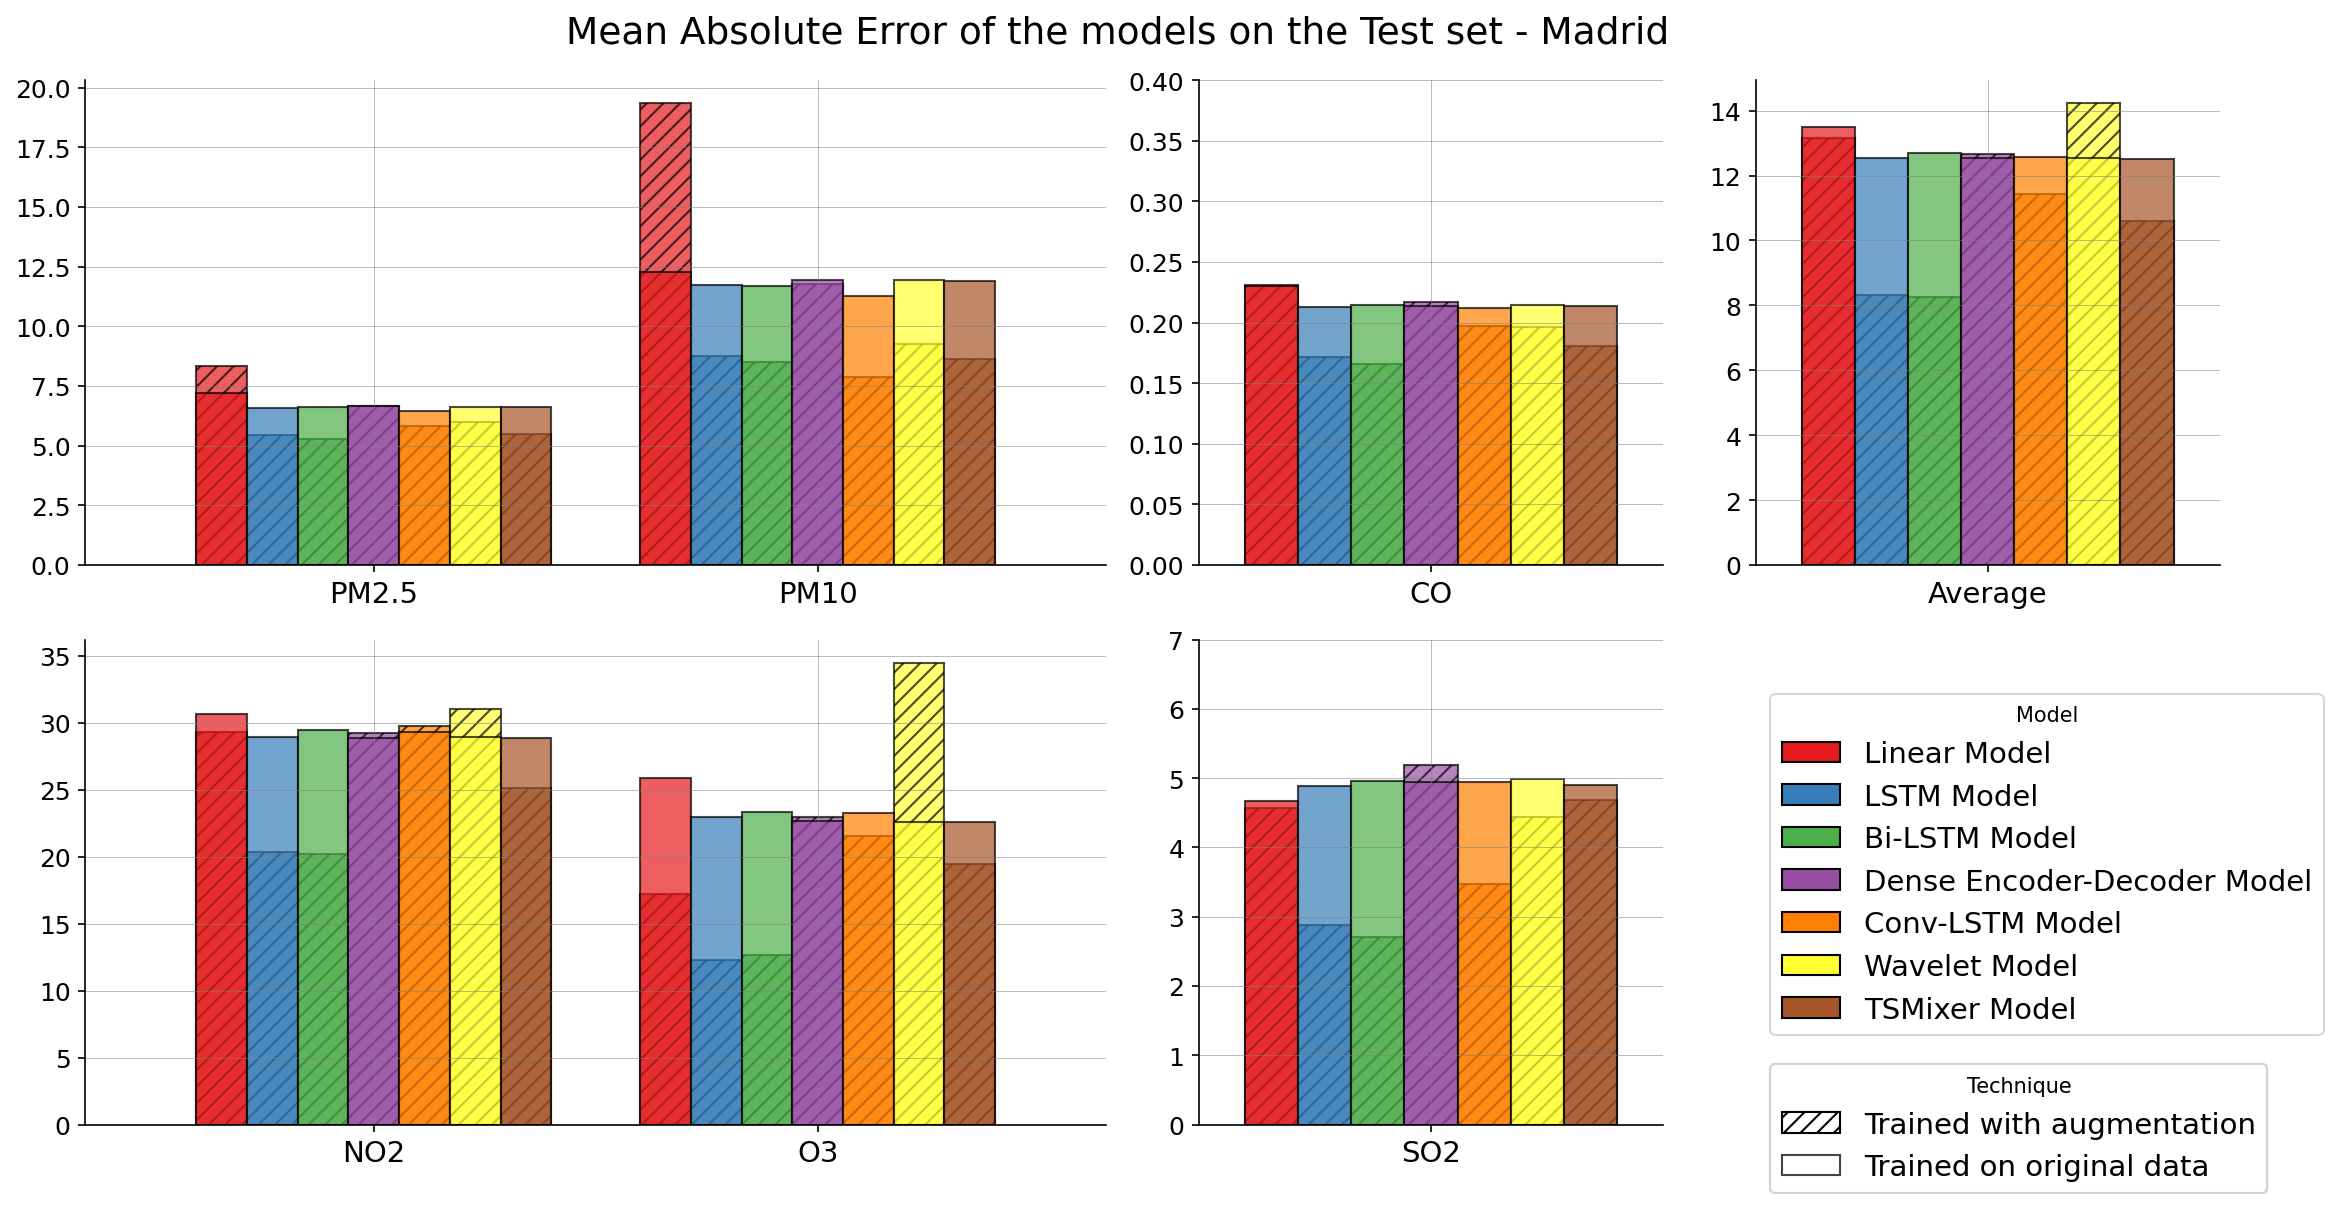
\includegraphics[width=1\linewidth]{images/Madrid_results.png}
    \caption{MAE on test set, for each model, divided by pollutant. The rightmost graph shows the average MAE of pollutants for each model. Hatched bars represent results after training with augmented data, while solid bars represent MAE without augmented data.}
    \label{fig:madrid_results}
\end{figure}

Once again, the Dense Encoder-Decoder model, which previously achieved the best MAE in the Aarhus dataset, is now among the three worst-performing models.
The difficulty encountered can be attributed to the quality of the Madrid dataset, which contains a significant amount of missing data and numerous outliers (as evidenced by the spikes observed in Section \ref{subsec:madrid-eda}). Furthermore, data augmentation does not significantly improve the results, as observed in other datasets, except for the LSTM and Bi-LSTM models, which consistently outperform other models in this experiment.

\begin{table}[]
    \centering
    \begin{tabular}{lcc}
        \toprule
        \textbf{Model} & \textbf{MAE} & \textbf{sMAPE} \\ 
        \midrule
        Linear & 13.17 & 64.3\% \\
        LSTM & 8.31 & 45.03\% \\
       \textbf{Bi-LSTM}& \textbf{8.25} & \textbf{43.95}\% \\
        Dense encoder decoder & 12.66 & 58.49\% \\
        CONV-LSTM & 11.44 & 52.23\% \\
        TSMixer & 10.58 & 51.72\% \\
        Wavelet & 14.23 & 58.02\% \\ 
        \bottomrule
    \end{tabular}
    \caption{Madrid models average performances, on augmented dataset models.}
    \label{tab:Madrid_performances}
\end{table}

The obtained results thus demonstrate a lower predictability of the Madrid dataset, highlighting the necessity for high data quality as well as a substantial amount of data (bearing in mind that in the case of Madrid a 3-year observation period was available).

\section{Best models comparison}

While in the previous section we have showed the performances of all tested models, in this section we will shortly analyze some aspects of the top performing models that should help us to pick the best one for our use case. Choosen top-performing models are the following:
\begin{itemize}
    \item LSTM model
    \item Bi-LSTM model
    \item Tsmixer
    \item Wavelet
\end{itemize}

In this section we will always refer to the results obtained after training with augmentation.

\subsection{Comparison with baseline}
\label{subsec:baseline_comparison}
The Mean Absolute Errors of the highest-performing models were juxtaposed with those obtained from the Autoregressive Integrated Moving Average (ARIMA) models. As elucidated in Section \ref{subsec:baseline}, the baseline's predictions were treated as multiple univariate forecasting problem. To facilitate comparison, the MAE derived from individual series was averaged. It is noteworthy that, in the majority of cases, the baseline tended to predict a linear trajectory, often corresponding to the series mean, rather than exhibiting the expected variability. This predictive behavior of the baseline could indeed contribute to the improvement of MAE.

A summary table (Table \ref{tab:baseline-comparison}) is presented below, delineating the models that surpassed the baseline performance across three datasets.

\begin{table}[]
\centering
\begin{tabular}{lccc}
\toprule
\textbf{Model/Dataset} & \textbf{Citypulse} & \textbf{Seoul} & \textbf{Madrid} \\ 
\midrule
ARIMA & 17.41 & 6.92 & 10.32 \\
LSTM & 9.18 & 2.51 & 8.31 \\
Bi-LSTM & 9.33 & 2.68 & 8.25 \\
TSMixer \cite{chen2023tsmixer} & 9.34 & 3.71 & \textbf{10.58} \\
Wavelet & 9.23 & 2.80 & \textbf{14.23} \\
\bottomrule
\end{tabular}
\caption{MAE table comparison with baseline.}
\label{tab:baseline-comparison}
\end{table}

Evidently, the selected models demonstrate superior performance relative to the baseline in both the Citypulse and Seoul datasets. Conversely, in the Madrid dataset, the TSMixer and Wavelet models fails to surpass the baseline, confirming their inferior performance.

\subsection{Error over time}

The forecast horizon is of course a choice that influences the performances of the models. In the case of one-step-ahead, the model would use the past observations to predict one observation, which would be a quite easy task. During multi-step forecast, the task becomes tricky for two reasons:
\begin{enumerate}
    \item The model has to use the same amount of past observations to predict a longer sequence of observations
    \item The error in one observation can propagate to the successive ones
\end{enumerate}

Of course, the more observations we try to predict, the larger the error.
In the following plot (Figure \ref{fig:mae-per-hour}) we have compared the error of each model, for each dataset, based on the temporal distance from the last observed value.

\begin{figure}
    \centering
    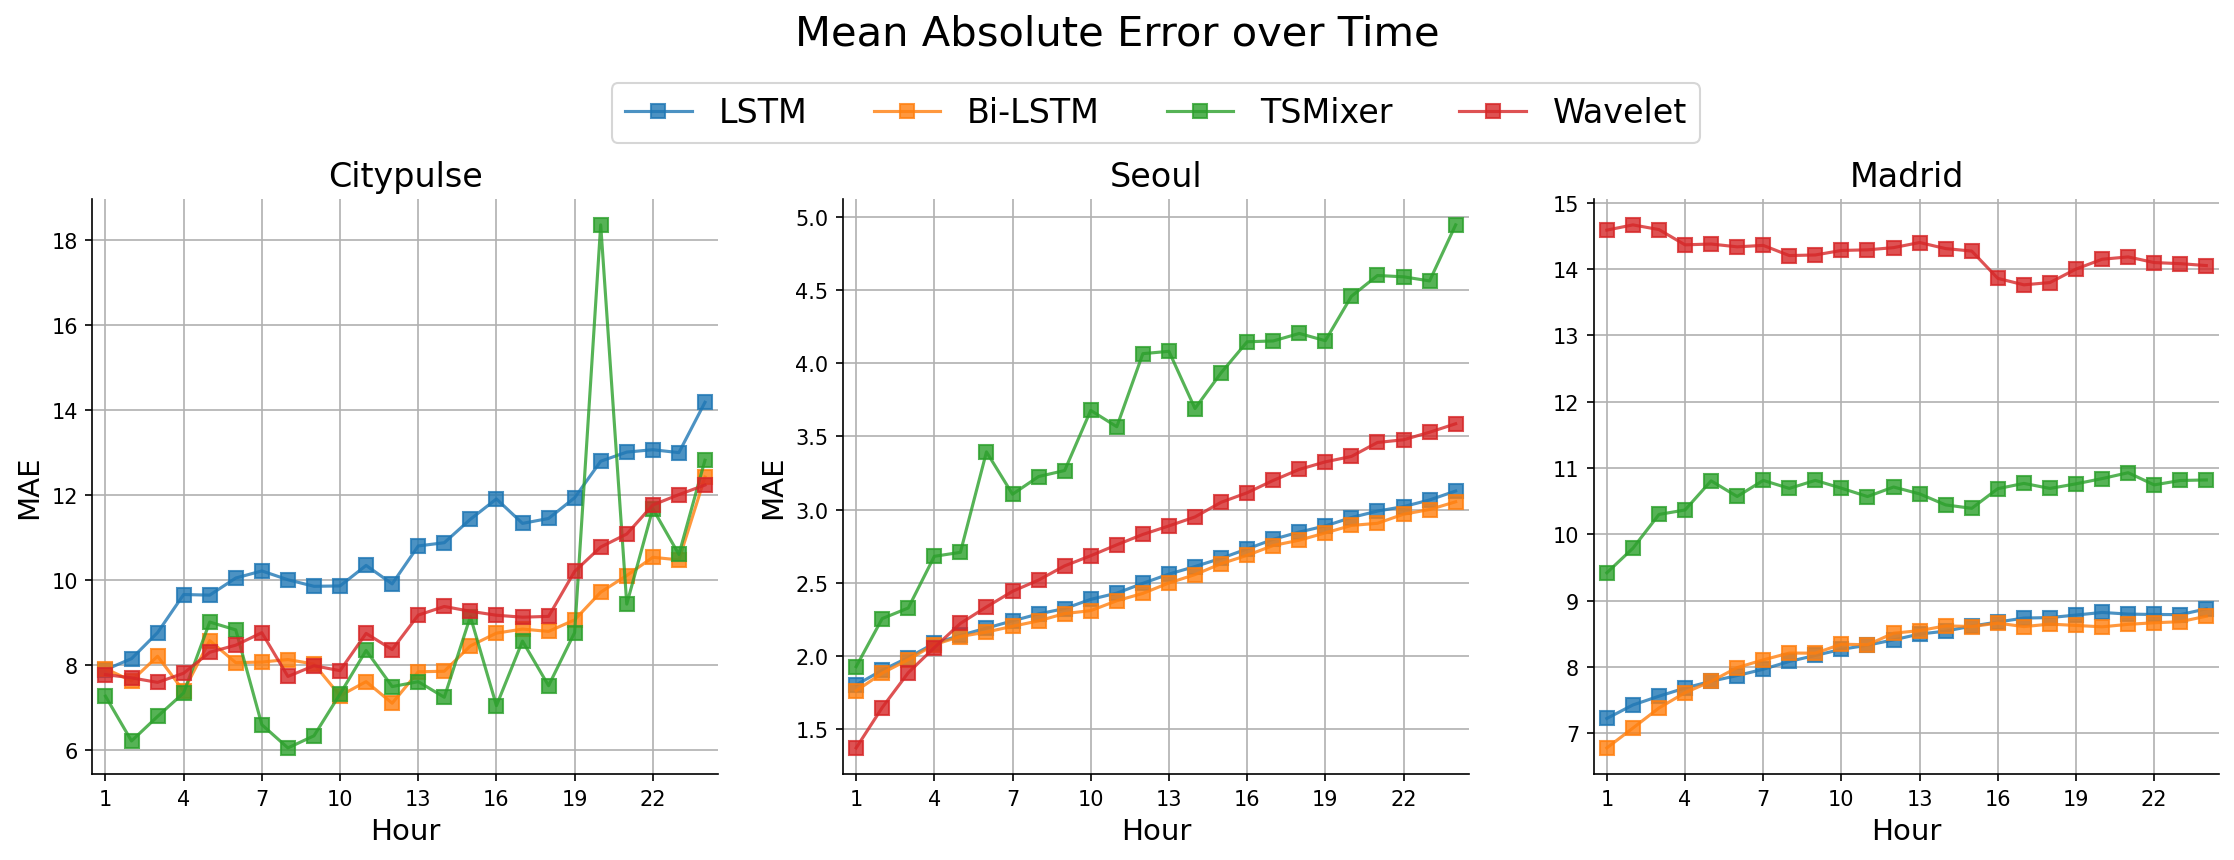
\includegraphics[width=1\linewidth]{images/mae_per_hour.png}
    \caption{MAE of each model based on the distance (in hours) from the last observed value.}
    \label{fig:mae-per-hour}
\end{figure}

Commencing with the Citypulse dataset, a discernible trend is observed, as anticipated, wherein the error exhibits a gradual increase over the forecast horizon. Notably, the Bi-LSTM and TSMixer models emerge as the two most proficient models in managing this aspect. However, while the error in the Bi-LSTM dataset displays a relatively uniform growth pattern, the TSMixer curve manifests substantial variability, casting doubt on the reliability of model predictions.

In the Seoul dataset, results are more transparent and interpretable. While the Wavelet model demonstrates superior predictive capabilities in the initial two observations, it is noteworthy that the error rapidly escalates until approximately the eighth observation. Subsequently, it exhibits a slow and linear growth. In contrast, the curves of the LSTM and Bi-LSTM models, which achieved the best results in terms of both MAE and sMAPE, are nearly overlapping. These models demonstrate a gradual linear worsening, with a minimal increase at the maximum forecast distance. On the other hand, the TSMixer model, despite starting with a relatively low error of approximately 2, deteriorates rapidly towards an error at the maximum distance equal to 5.

In the Madrid dataset, the performance of the LSTM and Bi-LSTM models is reaffirmed, as the error increases gradually with temporal distance. The TSMixer model also achieves an intermediate result, albeit inferior to the baseline (refer to Section \ref{subsec:baseline_comparison}). Conversely, the Wavelet model exhibits a peculiar trend. Despite a slight improvement, the error increases with temporal distance, deviating from the expected decrease. This outcome may be attributed more to chance than to a recognizable pattern.\\

After these considerations, the analysis will focus on the Bi-LSTM and the LSTM models, and we will then analyze the errors and will show some qualitative plots to better understand the behaviours of the two models.

\subsection{Error analysis}

In addition to Mean Absolute Error (MAE), which is a quantitative metric, another valuable approach for assessing errors involves examining the distribution of residuals. A residual is the difference between the predicted and actual values, and by plotting their distribution, insights into the model's performance can be gained. An ideal scenario is one where residuals are concentrated around zero, indicative of accurate predictions. Conversely, a shift in the distribution signals a tendency for the model to either overestimate or underestimate future values.

Figure \ref{fig:kde_residuals} illustrates the residual distributions for both Long Short-Term Memory (LSTM) and Bidirectional LSTM (Bi-LSTM) across the three datasets. Analyzing these distributions provides valuable insights into the models' tendencies to either overestimate or underestimate future values for each dataset.

\begin{figure}
    \centering
    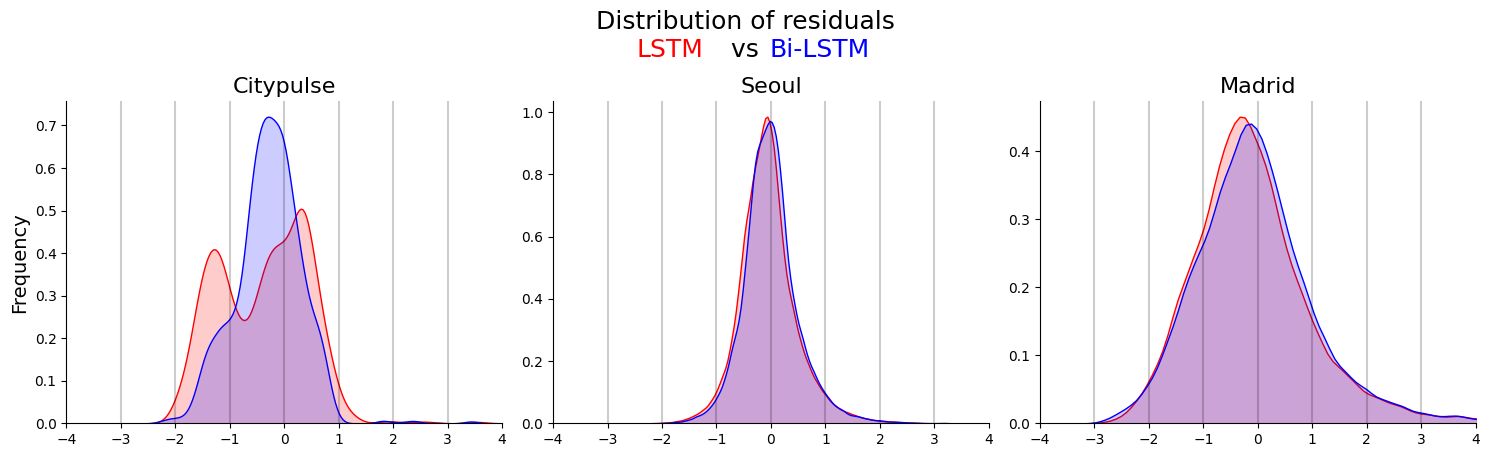
\includegraphics[width=1\linewidth]{images/Residuals_distribution.png}
    \caption{Distribution of residuals for each dataset, LSTM model (in red) and Bi-LSTM model (in blue)}
    \label{fig:kde_residuals}
\end{figure}

The results show differences between the models, especially in the CityPulse dataset. The Madrid and Seoul datasets have similar results for both the Bi-LSTM and LSTM models. In the CityPulse dataset, while the Bi-LSTM model's performance curve is skewed but mostly normal, the LSTM model shows a distribution with two peaks: one near zero and the other at -1.2. This indicates that the model accurately predicts some values while overestimating others.

The complexity of this phenomenon cannot be fully explained by the Mean Absolute Error (MAE), highlighting the need for this analysis. It can be argued that the accuracy of the first peak predictions compensates for the other peak prediction in the MAE calculation, resulting in a close approximation of the Bi-LSTM model's performance.

Next, we will provide concise visual representations of out-of-sample forecasts for both the Bi-LSTM and LSTM models. It is important to note that these plots should not be used as the sole criterion for determining the superior performance of a model. Instead, they should be considered a potential tool for gaining a better understanding of how the information extracted from the previous analysis applies in practice.

\paragraph{Citypulse}
From the plots in Figure \ref{fig:forecasts_aarhus}, we can see that while the Bi-LSTM model (in blue) doesn't fit very well with the predictions, the LSTM model gets better results in O\textsubscript{3} and PM\textsubscript{2.5} series, but overestimates both PM\textsubscript{10} and NO\textsubscript{2} series. If repeated, this pattern could explain the difference seen in the distribution of residuals.

\begin{figure}[h]
    \centering
    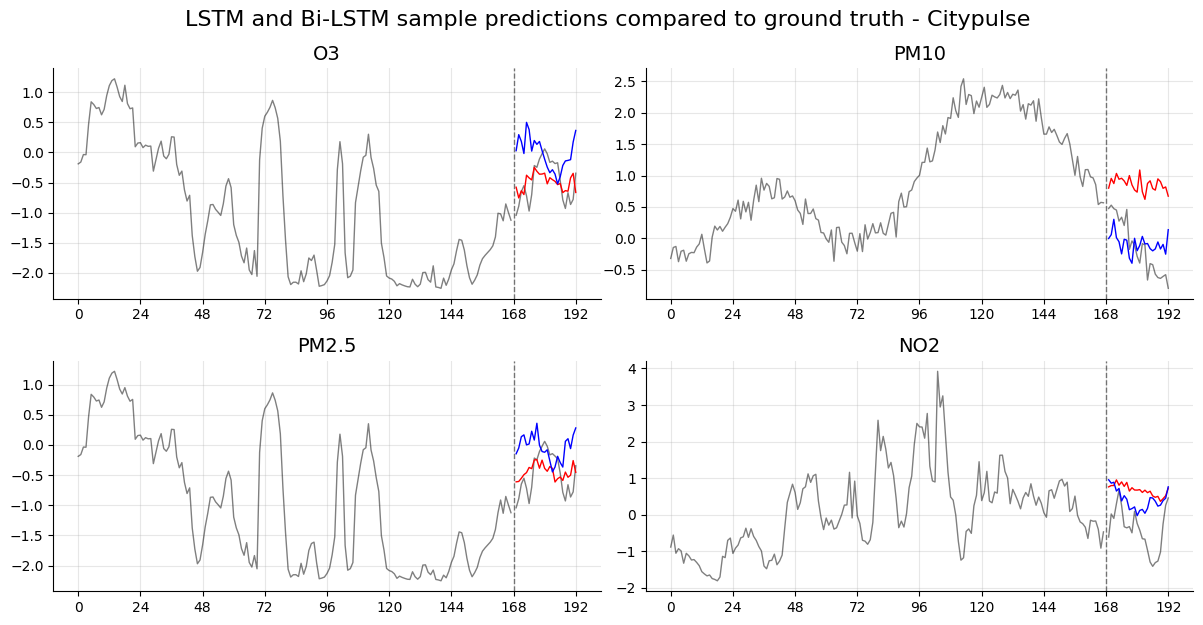
\includegraphics[width=1\linewidth]{images/forecasts_aarhus.png}
    \caption{Forecast of one time window extracted from the test set of Seoul dataset. Both models forecasts are displayed, LSTM (in red) and Bi-LSTM (in blue)}
    \label{fig:forecasts_aarhus}
\end{figure}

\paragraph{Seoul}

The predictions delineated in Figure \ref{fig:forecasts_seoul} elucidate a marked parity between the two models, evident in their capacity to encapsulate the overarching trend within the series. It is noteworthy that this congruence extends to both O\textsubscript{3} and CO predictions, wherein the forecasted trajectories closely mirror those of the original series.

\begin{figure}[h]
    \centering
    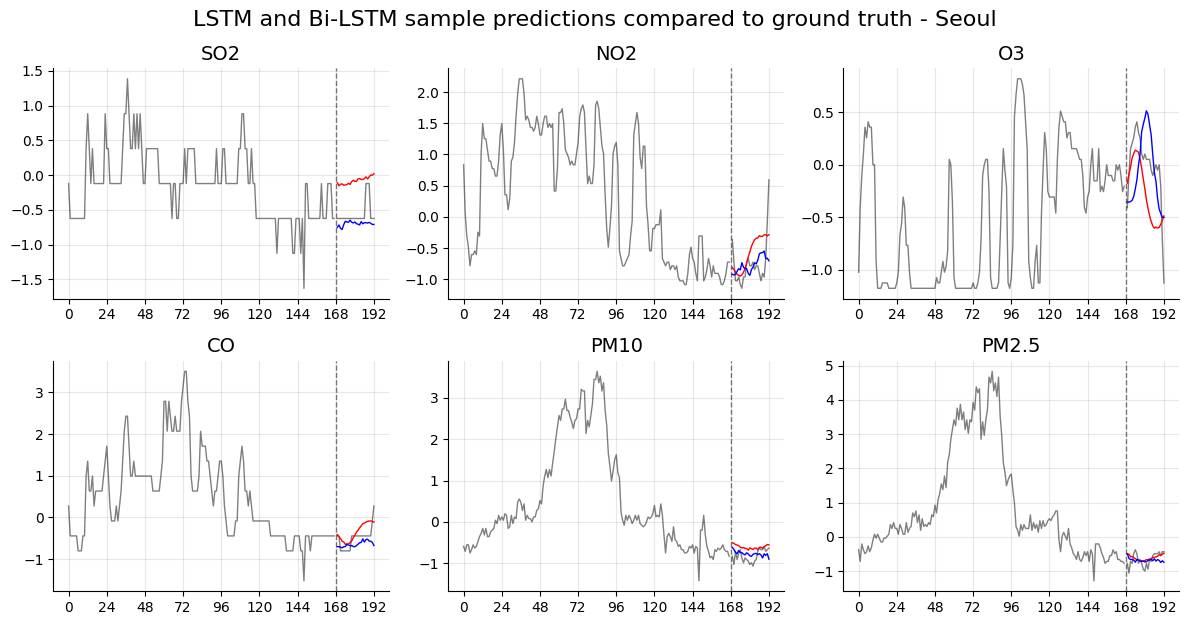
\includegraphics[width=1\linewidth]{images/forecasts_seoul.png}
    \caption{Forecast of one time window extracted from the test set of Seoul dataset. Both models forecasts are displayed, LSTM (in red) and Bi-LSTM (in blue)}
    \label{fig:forecasts_seoul}
\end{figure}

\paragraph{Madrid}
The dataset from Madrid exhibits the most variability, as shown in the plots in Figure \ref{fig:forecasts_Madrid}. However, the models provide a reasonably accurate approximation of future values, particularly the Bi-LSTM model. The SO\textsubscript{2} series has the poorest predicted values, as the models fail to accurately predict actual values. It is worth noting that the SO\textsubscript{2} series appears to have a step function shape, unlike the other series.

\begin{figure}[h]
    \centering
    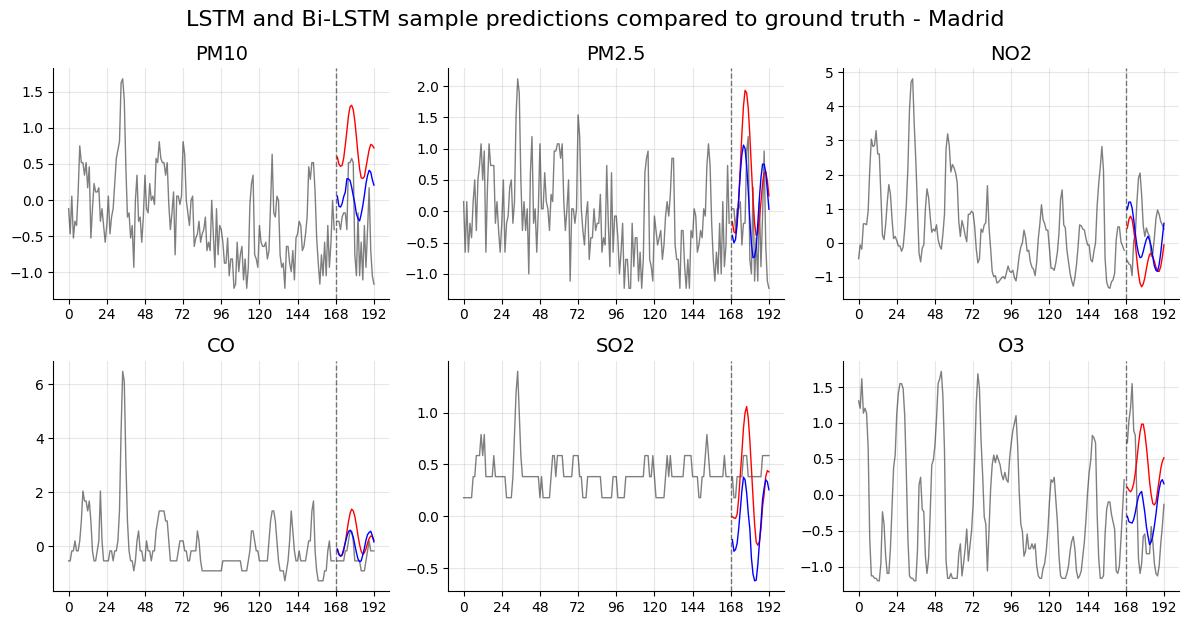
\includegraphics[width=1\linewidth]{images/forecasts_madrid.png}
    \caption{Forecast of one time window extracted from the test set of Madrid dataset. Both models forecasts are displayed, LSTM (in red) and Bi-LSTM (in blue)}
    \label{fig:forecasts_Madrid}
\end{figure}

\section{Results discussion}

In this research, seven models were tested on the three existing datasets. These experiments provided a more comprehensive understanding of the requirements for proficient time series prediction using deep learning models which are often referred to as black-boxes\footnote{This term is used to describe their lack of transparency in the decision-making process}.

\subsection*{Ablation studies}

The study shows that models that take into account temporal considerations, such as memory mechanisms (as seen in LSTM, Bi-LSTM, and Wavelet models) or features derived from the temporal dimension (as seen in TSMixer), consistently outperform other models in terms of predictive efficacy.

Various configurations of the data fed into the training phase have been tested:

\paragraph{Historical data volume influence}

As described in Section \ref{subsec:experiments}, we investigated the impact of historical data volume on the models trained on Seoul and Madrid datasets. Specifically, we compared the outcomes of models trained on a 1-year temporal span with those trained over a 3-year interval without augmentation. The results are presented in Figure \ref{fig:more_data_improv}.

\begin{figure}[h]
    \centering
    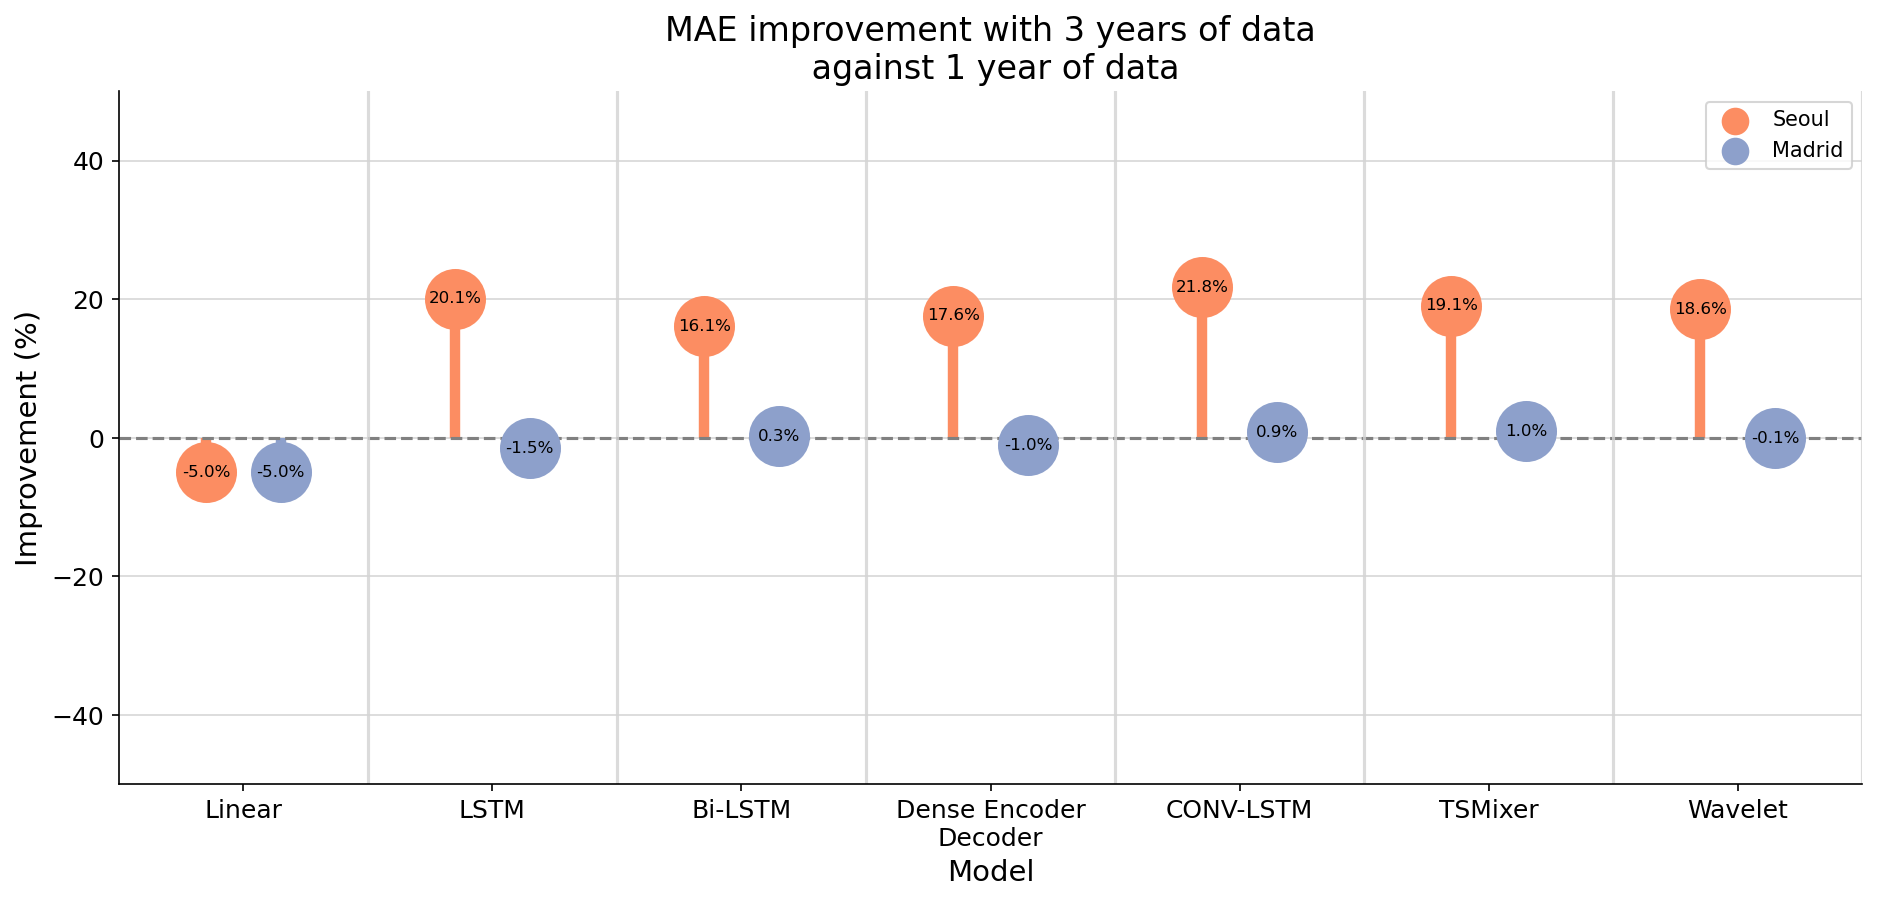
\includegraphics[width=1\linewidth]{images/improvement with more data.png}
    \caption{Reduction in MAE (\%) in models trained with 3 years of data, compared with that with 1 year of data.}
    \label{fig:more_data_improv}
\end{figure}

A clear improvement of approximately 20\% is evident across all models, except for the Linear model. This observation supports the claim that the simplicity of the Linear model hinders its adaptability to a non-uniform dataset. It is noteworthy that the other models benefit significantly from an expanded training dataset, with the CONV-LSTM model showing the most substantial improvement at 21.8\%. This result supports the idea that as the model becomes more complex, more training data is needed to achieve the best performance.

\paragraph{Data augmentation benefits}

In this chapter we have seen that data augmentation have brought benefits in the predictions. The following plot (Figure \ref{fig:augmentation-improv}) is used to better understand the impact of the implemented data augmentation on the results, for each model, in the three datasets.

\begin{figure}[h]
    \centering
    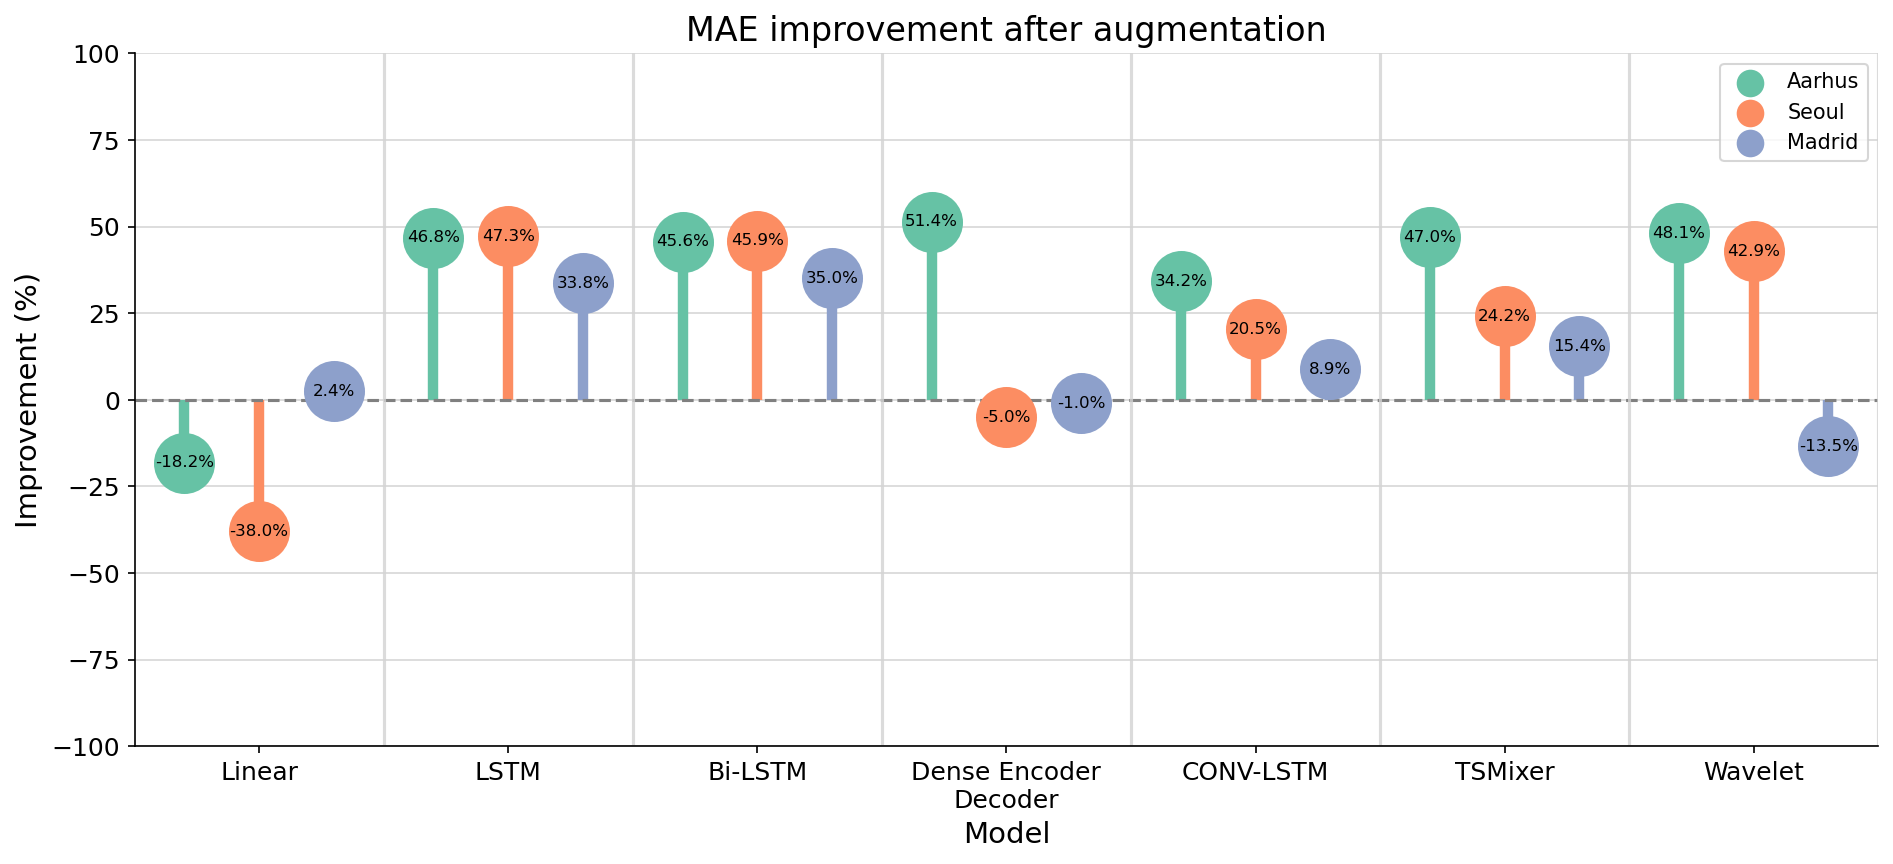
\includegraphics[width=1\linewidth]{images/improvement with augmentation.png}
    \caption{MAE reduction (\%) after data augmentation, for all models.}
    \label{fig:augmentation-improv}
\end{figure}

Despite the worstening in the linear model, for which we have already given an explanation in the previous sections, what we see is that overall the data augmentation confirms it's utility in the training process, with also reductions of almost -50\% in MAE. 






% VA NELLE CONCLUSIONI





\chapter{Conclusions}










\section*{Further developments}

The analysis and prediction of pollutant time series is an evolving field, and our current work provides a solid foundation for further development and refinement. Below, we explore some promising directions for the future of our research:

\paragraph{Optimization of Hyperparameters:}
To enhance the performance of our models, it is crucial to explore a broader range of hyperparameters. Testing various configurations of hyperparameters, including those related to model structure, activation functions, and learning rates, could lead to more robust models that are adaptable to a variety of contexts.

\paragraph{Variability in Data Augmentation:}
To increase diversity in the data, advanced data augmentation strategies can be employed. Rather than simply adding noise to each epoch, it could be implemented a solution that keeps the original data and generates different versions with varying noise intensities. This involves creating datasets, each characterized by distinct noise levels derived from normal distributions with different standard deviations. The aim of this approach is to increase the diversity of the data, which can improve the model's ability to generalize to unobserved data. However, due to computational limitations, this approach could not be attempted in this context.

\paragraph{Separate Loss Functions:}
Customizing loss functions for each pollutant is an important step in tailoring forecasts to the specific characteristics of different time series. Introducing separate loss functions could allow models to focus more on the specific dynamics of each pollutant, thereby improving the accuracy of forecasts.


\paragraph{Use of Space Data:}
The integration of spatial data offers a significant opportunity to enhance the accuracy of air pollution forecasts. Analyzing the spatial distribution of pollution sources and surrounding environmental factors can provide additional insights. The use of advanced spatial modeling techniques, such as Spatio-Temporal Graph Neural Networks, enables the prediction of pollutant values at a station by considering influences from surrounding areas. This approach contributes to a more comprehensive view of air quality, allowing for further refinement of predictions and the development of more effective strategies for environmental management and public health.


\appendix
\chapter{Appendix}
\label{app:a}

\section{Variable description}
Following are the description tables for each variable of the datasets used in this work.

\begin{table}[ht]
   
    \centering
    \begin{tabular}{|p{3cm}|p{9cm}|}
        \hline
        \textbf{Field} & \textbf{Description} \\
        \hline
        timestamp & Date and time of observations with a sampling interval of 5 minutes, covering the period from August 2014 to October 2014. \\
        vehicleCount & Number of vehicles counted in a specific time interval. \\ 
        avgSpeed & Average speed of vehicles in the specific time interval. \\ 
        totalspaces & Total number of parking spaces available in the area. \\ 
        occupied & Number of parking spaces occupied at a given moment. \\ 
        occupancy & Percentage of parking spaces occupied relative to the total available. \\ 
        temp & Ambient temperature recorded at the observation location. \\ 
        feelslike & Apparent temperature, taking into account temperature and other meteorological factors. \\ 
        humidity & Percentage of humidity in the air. \\ 
        precip & Amount of precipitation recorded during the observation period. \\ 
        precipprob & Probability of precipitation in the specific time interval. \\ 
        windspeed & Wind speed in the observation area. \\ 
        cloudcover & Cloud cover in the sky, expressed as a percentage. \\ 
        visibility & Visibility distance in meters. \\ 
        ozone & Ozone concentration in the air, measured in specific units. \\ 
        pm10 & Concentration of PM10 particulate matter in the air, measured in specific units. \\ 
        pm25 & Concentration of PM2.5 particulate matter in the air, measured in specific units. \\ 
        no2 & Concentration of nitrogen dioxide (NO\textsubscript{2}) in the air, measured in specific units. \\ 
        \hline
    \end{tabular}
    \caption{CityPulse dataset columns description}
     \label{apptable:Citypulse_variable_descriptio}
\end{table}

\begin{table}[ht]
    
    \centering
    \begin{tabular}{|p{3cm}|p{9cm}|}
        \hline
        \textbf{Variable} & \textbf{Description} \\
        \hline
        SO2 & Concentration of sulfur dioxide (SO\textsubscript{2}) in the air, measured in specific units. \\
        NO2 & Concentration of nitrogen dioxide (NO\textsubscript{2}) in the air, measured in specific units. \\
        O3 & Ozone concentration in the air, measured in specific units. \\
        CO & Concentration of carbon monoxide (CO) in the air, measured in specific units. \\
        PM10 & Concentration of PM\textsubscript{10} particulate matter in the air, measured in specific units. \\
        PM2.5 & Concentration of PM\textsubscript{2.5} particulate matter in the air, measured in specific units. \\
        temp & Ambient temperature recorded at the observation location. \\
        humidity & Percentage of humidity in the air. \\
        prec & Amount of precipitation recorded during the observation period. \\
        rain & Amount of rain recorded during the observation period. \\
        snow & Amount of snow recorded during the observation period. \\
        cloudcover & Cloud cover in the sky, expressed as a percentage. \\
        wind\_speed & Wind speed in the observation area. \\
        \hline
    \end{tabular}
    \caption{Seoul dataset columns description}
    \label{apptable:Seoul_variable_description}
\end{table}


\begin{table}[ht]

    \centering
    \begin{tabular}{|p{3cm}|p{9cm}|}
        \hline
        \textbf{Variable} & \textbf{Description} \\
        \hline
        PM10 & Concentration of PM\textsubscript{10} particulate matter in the air, measured in specific units. \\
        PM2.5 & Concentration of PM\textsubscript{2.5} particulate matter in the air, measured in specific units. \\
        NO2 & Concentration of nitrogen dioxide (NO\textsubscript{2}) in the air, measured in specific units. \\
        CO & Concentration of carbon monoxide (CO) in the air, measured in specific units. \\
        SO2 & Concentration of sulfur dioxide (SO\textsubscript{2}) in the air, measured in specific units. \\
        O3 & Ozone concentration in the air, measured in specific units. \\
        temp & Ambient temperature recorded at the observation location. \\
        humidity & Percentage of humidity in the air. \\
        dew & Dew point temperature, representing the temperature at which air becomes saturated and dew forms. \\
        prec & Amount of precipitation recorded during the observation period. \\
        rain & Amount of rain recorded during the observation period. \\
        snow & Amount of snow recorded during the observation period. \\
        pressure & Atmospheric pressure at the observation location. \\
        cloudcover & Cloud cover in the sky, expressed as a percentage. \\
        wind\_speed & Wind speed in the observation area. \\
        wind\_dir & Wind direction, indicating the compass direction from which the wind is blowing. \\
        \hline
    \end{tabular}
    \caption{Seoul dataset columns description}
    \label{apptable:madrid_variable_description}
\end{table}






%%%%%%%%%%%%%%%%%%%%%%%%%%%%%%%%%%%%%%%%%%%%%%%%%%%%%%%%%%%%%%%

% BIBLIOGRAFIA
\phantomsection
\printbibliography[type=article,title={Bibliography}, heading=bibintoc]
\printbibliography[type=online,title={Web references}, heading=bibintoc]

%%%%%%%%%%%%%%%%%%%%%%%%%%%%%%%%%%%%%%%%%%%%%%%%%%%%%%%%%%%%%%%

% RINGRAZIAMENTI - PERSONALIZZARE

\ringraziamenti
\addcontentsline{toc}{chapter}{Aknowledgments}
I express my gratitude to the University of Milano-Bicocca, particularly the Department of Computer Science, Systems and Communication, for the stimulating environment and educational opportunities provided during these 5 unforgettable years.\\

\noindent
I would like to thank Professors Simone Bianco and Paolo Napoletano, thesis advisors, for their guidance during the course of this project. Special thanks to Dr. Luigi Celona, co-referee of the thesis, for his support in the development of the project and his suggestions. His contribution was indispensable for the success of this work.\\

\noindent
Sono per sempre grato ai miei genitori per avermi dato la possibilità di fare questo percorso, nonostante i sacrifici. Malumori e sorrisi, vi voglio bene e siete parte fondamentale di me, ovunque io sia.\\

\noindent
Ringrazio mia sorella per essere sempre una sponda sicura con cui confrontarsi, anche nelle difficoltà di questo percorso.\\

\noindent
Grazie ai miei amici, in particolare Bartolo, per conoscermi a fondo e capirmi. Ringrazio chiunque mi sia stato vicino in questi anni, per un conforto o per una risata. \\

\noindent
Infine grazie a Elisa, per ciò che sei.





%%%%%%%%%%%%%%%%%%%%%%%%%%%%%%%%%%%%%%%%%%%%%%%%%%%%%%%%%%%%%%%

\end{document}